% !TeX spellcheck = russian-aot-ieyo
% Зачем: Определяет класс документа (То, как будет выглядеть документ)
% Примечание: параметр draft помечает строки, вышедшие за границы страницы, прямоугольником, в фильной версии его нужно удалить.
\documentclass[a4paper,14pt,russian,oneside,final]{extreport}

% Зачем: Настройка Times New Roman.
% Рекомендовано для Windows (нужен PSCyr, подробности см. в fonts_windows.tex)
% раскомментировать, чтобы использовать:
% Зачем: Предоставляет проприетарный Times New Roman.
% ОБНОВЛЕНИЕ: лучше использовать scalable-cyrfonts-tex: меньше проблем с установкой
% Из руководства к PSCyr: "Во избежание проблем пакет PSCyr должен загружаться перед пакета-ми inputenc и babel".
% Примечание: Требует шаманства при установке, инструкция http://plumbum-blog.blogspot.com/2010/06/miktex-28-pscyr-04d.html
% http://blog.harrix.org/?p=444
\usepackage{pscyr}

% Зачем: Выбор внутренней TeX кодировки.
\usepackage[T2A]{fontenc}

% не забудьте закомментировать % Зачем: Выбор внутренней TeX кодировки.
\usepackage[T2A]{fontenc}

% Зачем: Предоставляет свободный Times New Roman.
% Шрифт идёт вместе с пакетом scalable-cyrfonts-tex в Ubuntu/Debian

% пакет scalable-cyrfonts-tex может конфликтовать с texlive-fonts-extra в Ubuntu
% решение: Для себя я решил эту проблему так: пересобрал пакет scalable-cyrfonts-tex, изменив его имя. Решение топорное, но работает. Желающие могут скачать мой пакет здесь:
% https://yadi.sk/d/GW2PhDgEcJH7m
% Установка:
% dpkg -i scalable-cyrfonts-tex-shurph_4.16_all.deb

\usefont{T2A}{ftm}{m}{sl}


% Рекомендовано для Linux (нужен scalable-cyrfonts-tex, подробности см. в fonts_linux.tex)
% раскомментировать, чтобы использовать:
%% Зачем: Выбор внутренней TeX кодировки.
\usepackage[T2A]{fontenc}

% Зачем: Предоставляет свободный Times New Roman.
% Шрифт идёт вместе с пакетом scalable-cyrfonts-tex в Ubuntu/Debian

% пакет scalable-cyrfonts-tex может конфликтовать с texlive-fonts-extra в Ubuntu
% решение: Для себя я решил эту проблему так: пересобрал пакет scalable-cyrfonts-tex, изменив его имя. Решение топорное, но работает. Желающие могут скачать мой пакет здесь:
% https://yadi.sk/d/GW2PhDgEcJH7m
% Установка:
% dpkg -i scalable-cyrfonts-tex-shurph_4.16_all.deb

\usefont{T2A}{ftm}{m}{sl}
% не забудьте закомментировать % Зачем: Предоставляет проприетарный Times New Roman.
% ОБНОВЛЕНИЕ: лучше использовать scalable-cyrfonts-tex: меньше проблем с установкой
% Из руководства к PSCyr: "Во избежание проблем пакет PSCyr должен загружаться перед пакета-ми inputenc и babel".
% Примечание: Требует шаманства при установке, инструкция http://plumbum-blog.blogspot.com/2010/06/miktex-28-pscyr-04d.html
% http://blog.harrix.org/?p=444
\usepackage{pscyr}

% Зачем: Выбор внутренней TeX кодировки.
\usepackage[T2A]{fontenc}



% Зачем: Установка кодировки исходных файлов.
\usepackage[utf8]{inputenc}

% Зачем: Делает результирующий PDF "searchable and copyable".
\usepackage{cmap}

% Зачем: Чтобы можно было использовать русские буквы в формулах, но в случае использования предупреждать об этом.
\usepackage[warn]{mathtext}

% Зачем: Учет особенностей различных языков.
\usepackage[russian]{babel}

% Зачем: Добавляет поддержу дополнительных размеров текста 8pt, 9pt, 10pt, 11pt, 12pt, 14pt, 17pt, and 20pt.
% Почему: Пункт 2.1.1 Требований по оформлению пояснительной записки.
\usepackage{extsizes}


% Зачем: Длинна, пимерно соответвующая 5 символам
% Почему: Требования содержат странное требование про отсупы в 5 символов (для немоноширинного шрифта :| )
\newlength{\fivecharsapprox}
\setlength{\fivecharsapprox}{6ex}


% Зачем: Добавляет отступы для абзацев.
% Почему: Пункт 2.1.3 Требований по оформлению пояснительной записки.
\usepackage{indentfirst}
\setlength{\parindent}{\fivecharsapprox} % Примерно соответсвует 5 символам.


% Зачем: Настраивает отступы от границ страницы.
% Почему: Пункт 2.1.2 Требований по оформлению пояснительной записки.
\usepackage[left=3cm,top=2.0cm,right=1.5cm,bottom=2.7cm]{geometry}


% Зачем: Настраивает межстрочный интервал, для размещения 40 +/- 3 строки текста на странице.
% Почему: Пункт 2.1.1 Требований по оформлению пояснительной записки.
\usepackage[nodisplayskipstretch]{setspace} 
\setstretch{1.1}
%\onehalfspacing

% Зачем: Выбор шрифта по-умолчанию. 
% Почему: Пункт 2.1.1 Требований по оформлению пояснительной записки.
% Примечание: В требованиях не указан, какой именно шрифт использовать. По традиции используем TNR.
\renewcommand{\rmdefault}{ftm} % Times New Roman


% Зачем: Отключает использование изменяемых межсловных пробелов.
% Почему: Так не принято делать в текстах на русском языке.
\frenchspacing


% Зачем: Сброс счетчика сносок для каждой страницы
% Примечание: в "Требованиях по оформлению пояснительной записки" не указано, как нужно делать, но в других БГУИРовских докуметах рекомендуется нумерация отдельная для каждой страницы
\usepackage{perpage}
\MakePerPage{footnote}


% Зачем: Добавляет скобку 1) к номеру сноски
% Почему: Пункты 2.9.2 и 2.9.1 Требований по оформлению пояснительной записки.
\makeatletter 
\def\@makefnmark{\hbox{\@textsuperscript{\normalfont\@thefnmark)}}}
\makeatother


% Зачем: Расположение сносок внизу страницы
% Почему: Пункт 2.9.2 Требований по оформлению пояснительной записки.
\usepackage[bottom]{footmisc}


% Зачем: Переопределяем стандартную нумерацию, т.к. в отчете будут только section и т.д. в терминологии TeX
\makeatletter
\renewcommand{\thesection}{\bfseries\arabic{section}}
\makeatother


% Зачем: Пункты (в терминологии требований) в терминологии TeX subsubsection должны нумероваться
% Почему: Пункт 2.2.3 Требований по оформлению пояснительной записки.
\setcounter{secnumdepth}{3}


% Зачем: Настраивает отступ между таблицей с содержанимем и словом СОДЕРЖАНИЕ
% Почему: Пункт 2.2.7 Требований по оформлению пояснительной записки.
\usepackage{tocloft}
\setlength{\cftbeforetoctitleskip}{-1em}
\setlength{\cftaftertoctitleskip}{1em}


% Зачем: Определяет отступы слева для записей в таблице содержания.
% Почему: Пункт 2.2.7 Требований по оформлению пояснительной записки.
\makeatletter
\renewcommand{\l@section}{\@dottedtocline{1}{0.5em}{1.2em}}
\renewcommand{\l@subsection}{\@dottedtocline{2}{1.7em}{2.0em}}
\makeatother


% Зачем: Работа с колонтитулами
\usepackage{fancyhdr} % пакет для установки колонтитулов
\pagestyle{fancy} % смена стиля оформления страниц


% Зачем: Нумерация страниц располагается справа снизу страницы
% Почему: Пункт 2.2.8 Требований по оформлению пояснительной записки.
\fancyhf{} % очистка текущих значений
\fancyfoot[R]{\thepage} % установка верхнего колонтитула
\renewcommand{\footrulewidth}{0pt} % убрать разделительную линию внизу страницы
\renewcommand{\headrulewidth}{0pt} % убрать разделительную линию вверху страницы
\fancypagestyle{plain}{ 
    \fancyhf{}
    \rfoot{\thepage}}


% Зачем: Задает стиль заголовков раздела жирным шрифтом, прописными буквами, без точки в конце
% Почему: Пункты 2.1.1, 2.2.5, 2.2.6 и ПРИЛОЖЕНИЕ Л Требований по оформлению пояснительной записки.
\makeatletter
\renewcommand\section{%
  \clearpage\@startsection {section}{1}%
    {\fivecharsapprox}%
    {-1em \@plus -1ex \@minus -.2ex}%
    {1em \@plus .2ex}%
    {\raggedright\hyphenpenalty=10000\normalfont\large\bfseries\MakeUppercase}}
\makeatother


% Зачем: Задает стиль заголовков подразделов
% Почему: Пункты 2.1.1, 2.2.5 и ПРИЛОЖЕНИЕ Л Требований по оформлению пояснительной записки.
\makeatletter
\renewcommand\subsection{%
  \@startsection{subsection}{2}%
    {\fivecharsapprox}%
    {-1em \@plus -1ex \@minus -.2ex}%
    {1em \@plus .2ex}%
    {\raggedright\hyphenpenalty=10000\normalfont\normalsize}}
\makeatother


% Зачем: Задает стиль заголовков пунктов
% Почему: Пункты 2.1.1, 2.2.5 и ПРИЛОЖЕНИЕ Л Требований по оформлению пояснительной записки.
\makeatletter
\renewcommand\subsubsection{
  \@startsection{subsubsection}{3}%
    {\fivecharsapprox}%
    {-1em \@plus -1ex \@minus -.2ex}%
    {\z@}%
    {\raggedright\hyphenpenalty=10000\normalfont\normalsize}}
\makeatother

% Зачем: для оформления введения и заключения, они должны быть выровнены по центру.
% Почему: Пункты 1.1.15 и 1.1.11 Требований по оформлению пояснительной записки.
\makeatletter
\newcommand\sectioncentered{%
  \clearpage\@startsection {section}{1}%
    {\z@}%
    {-1em \@plus -1ex \@minus -.2ex}%
    {1em \@plus .2ex}%
    {\centering\hyphenpenalty=10000\normalfont\large\bfseries\MakeUppercase}%
    }
\makeatother



% Зачем: Задает стиль библиографии
% Почему: Пункт 2.8.6 Требований по оформлению пояснительной записки.
\bibliographystyle{styles/belarus-specific-utf8gost780u}


% Зачем: Пакет для вставки картинок
% Примечание: Объяснение, зачем final - http://tex.stackexchange.com/questions/11004/why-does-the-image-not-appear
\usepackage[final]{graphicx}
\DeclareGraphicsExtensions{.pdf,.png,.jpg,.eps}


% Зачем: Директория в которой будет происходить поиск картинок
\graphicspath{{figures/}}


% Зачем: Добавление подписей к рисункам
\usepackage[nooneline]{caption}
\usepackage{subcaption}

% Зачем: чтобы работала \No в новых латехах
\DeclareRobustCommand{\No}{\ifmmode{\nfss@text{\textnumero}}\else\textnumero\fi}

% Зачем: поворот ячеек таблиц на 90 градусов
\usepackage{rotating}
\DeclareRobustCommand{\povernut}[1]{\begin{sideways}{#1}\end{sideways}}


% Зачем: когда в формулах много кириллических символов команда \text{} занимает много места
\DeclareRobustCommand{\x}[1]{\text{#1}}


% Зачем: Задание подписей, разделителя и нумерации частей рисунков
% Почему: Пункт 2.5.5 Требований по оформлению пояснительной записки.
\DeclareCaptionLabelFormat{stbfigure}{Рисунок #2}
\DeclareCaptionLabelFormat{stbtable}{Таблица #2}
\DeclareCaptionLabelSeparator{stb}{~--~}
\captionsetup{labelsep=stb}
\captionsetup[figure]{labelformat=stbfigure,justification=centering}
\captionsetup[table]{labelformat=stbtable,justification=raggedright}
\renewcommand{\thesubfigure}{\asbuk{subfigure}}

% Зачем: Окружения для оформления формул
% Почему: Пункт 2.4.7 требований по оформлению пояснительной записки и специфические требования различных кафедр
% Пример использования смотри в course_content.tex, строка 5
\usepackage{calc}
\newlength{\lengthWordWhere}
\settowidth{\lengthWordWhere}{где}
\newenvironment{explanationx}
    {%
    %%% Следующие строки определяют специфические требования разных редакций стандартов. Раскоменнтируйте нужную строку
    %% стандартный абзац, СТП-01 2010
    %\begin{itemize}[leftmargin=0cm, itemindent=\parindent + \lengthWordWhere + \labelsep, labelsep=\labelsep]
    %% без отступа, СТП-01 2013
    \begin{itemize}[leftmargin=0cm, itemindent=\lengthWordWhere + \labelsep , labelsep=\labelsep]%
    \renewcommand\labelitemi{}%
    }
    {%
    %\\[\parsep]
    \end{itemize}
    }

% Старое окружение для "где". Сохранено для совместимости
\usepackage{tabularx}

\newenvironment{explanation}
    {
    %%% Следующие строки определяют специфические требования разных редакций стандартов. Раскоменнтируйте нужные 2 строки
    %% стандартный абзац, СТП-01 2010
    %\par 
    %\tabularx{\textwidth-\fivecharsapprox}{@{}ll@{ --- } X }
    %% без отступа, СТП-01 2013
    \noindent 
    \tabularx{\textwidth}{@{}ll@{ --- } X }
    }
    { 
    \\[\parsep]
    \endtabularx
    }


% Зачем: Удобная вёрстка многострочных формул, масштабирующийся текст в формулах, формулы в рамках и др
\usepackage{amsmath}


% Зачем: Поддержка ажурного и готического шрифтов 
\usepackage{amsfonts}


% Зачем: amsfonts + несколько сотен дополнительных математических символов
\usepackage{amssymb}


% Зачем: Окружения «теорема», «лемма»
\usepackage{amsthm}


% Зачем: Производить арифметические операции во время компиляции TeX файла
\usepackage{calc}

% Зачем: Производить арифметические операции во время компиляции TeX файла
\usepackage{fp}

% Зачем: Пакет для работы с перечислениями
\usepackage{enumitem}
\makeatletter
 \AddEnumerateCounter{\asbuk}{\@asbuk}{щ)}
\makeatother


% Зачем: Устанавливает символ начала простого перечисления
% Почему: Пункт 2.3.5 Требований по оформлению пояснительной записки.
\setlist{nolistsep}


% Зачем: Устанавливает символ начала именованного перечисления
% Почему: Пункт 2.3.8 Требований по оформлению пояснительной записки.
\renewcommand{\labelenumi}{\asbuk{enumi})}
\renewcommand{\labelenumii}{\arabic{enumii})}

% Зачем: Устанавливает отступ от границы документа до символа списка, чтобы этот отступ равнялся отступу параграфа
% Почему: Пункт 2.3.5 Требований по оформлению пояснительной записки.

\setlist[itemize,0]{itemindent=\parindent + 2.2ex,leftmargin=0ex,label=--}
\setlist[enumerate,1]{itemindent=\parindent + 2.7ex,leftmargin=0ex}
\setlist[enumerate,2]{itemindent=\parindent + \parindent - 2.7ex}

% Зачем: Включение номера раздела в номер формулы. Нумерация формул внутри раздела.
\AtBeginDocument{\numberwithin{equation}{section}}

% Зачем: Включение номера раздела в номер таблицы. Нумерация таблиц внутри раздела.
\AtBeginDocument{\numberwithin{table}{section}}

% Зачем: Включение номера раздела в номер рисунка. Нумерация рисунков внутри раздела.
\AtBeginDocument{\numberwithin{figure}{section}}


% Зачем: Дополнительные возможности в форматировании таблиц
\usepackage{makecell}
\usepackage{multirow}
\usepackage{array}


% Зачем: "Умная" запятая в математических формулах. В дробных числах не добавляет пробел
% Почему: В требованиях не нашел, но в русском языке для дробных чисел используется {,} а не {.}
\usepackage{icomma}

% Зачем: макрос для печати римских чисел
\makeatletter
\newcommand{\rmnum}[1]{\romannumeral #1}
\newcommand{\Rmnum}[1]{\expandafter\@slowromancap\romannumeral #1@}
\makeatother


% Зачем: Управление выводом чисел.
\usepackage{sistyle}
\SIdecimalsign{,}

% Зачем: inline-коментирование содержимого.
\newcommand{\ignore}[2]{\hspace{0in}#2}


% Зачем: Возможность коментировать большие участки документа
\usepackage{verbatim}


\usepackage{xcolor}


% Зачем: Оформление листингов кода
% Примечание: final нужен для переопределения режима draft, в котором листинги не выводятся в документ.
\usepackage[final]{listings}


% Зачем: настройка оформления листинга для языка F#
\definecolor{bluekeywords}{rgb}{0.13,0.13,1}
\definecolor{greencomments}{rgb}{0,0.5,0}
\definecolor{turqusnumbers}{rgb}{0.17,0.57,0.69}
\definecolor{redstrings}{rgb}{0.5,0,0}

\renewcommand{\lstlistingname}{Листинг}

\lstdefinelanguage{FSharp}
    {morekeywords={abstract,and,as,assert,base,begin,class,default,delegate,do,done,downcast,downto,elif,else,end,exception,extern,false,finally,for,fun,function,global,if,in,inherit,inline,interface,internal,lazy,let,let!,match,member,module,mutable,namespace,new,not,null,of,open,or,override,private,public,rec,return,return!,select,static,struct,then,to,true,try,type,upcast,use,use!,val,void,when,while,with,yield,yield!,asr,land,lor,lsl,lsr,lxor,mod,sig,atomic,break,checked,component,const,constraint,constructor,continue,eager,event,external,fixed,functor,include,method,mixin,object,parallel,process,protected,pure,sealed,tailcall,trait,virtual,volatile},
    keywordstyle=\bfseries\color{bluekeywords},
    sensitive=false,
    morecomment=[l][\color{greencomments}]{///},
    morecomment=[l][\color{greencomments}]{//},
    morecomment=[s][\color{greencomments}]{{(*}{*)}},
    morestring=[b]",
    stringstyle=\color{redstrings},
    }

\lstdefinestyle{fsharpstyle}{
   xleftmargin=0ex,
   language=FSharp,
   basicstyle=\footnotesize\ttfamily,
   breaklines=true,
   columns=fullflexible
}

\lstdefinestyle{csharpinlinestyle} {
  language=[Sharp]C,
  morekeywords={yield,var,get,set,from,select,partial,where,async,await},
  breaklines=true,
  columns=fullflexible,
  basicstyle=\footnotesize\ttfamily
}

\lstdefinestyle{csharpstyle}{
  language=[Sharp]C,
  frame=lr,
  rulecolor=\color{blue!80!black}}


% Зачем: Нумерация листингов в пределах секции
\AtBeginDocument{\numberwithin{lstlisting}{section}}

\usepackage[normalem]{ulem}

\usepackage[final,hidelinks]{hyperref}
% Моноширинный шрифт выглядит визуально больше, чем пропорциональный шрифт, если их размеры одинаковы. Искусственно уменьшаем размер ссылок.
\renewcommand{\UrlFont}{\small\rmfamily\tt}

\usepackage[square,numbers,sort&compress]{natbib}
\setlength{\bibsep}{0em}

% Магия для подсчета разнообразных объектов в документе
\usepackage{lastpage}
\usepackage{totcount}
\regtotcounter{section}

\usepackage{etoolbox}

\newcounter{totfigures}
\newcounter{tottables}
\newcounter{totreferences}
\newcounter{totequation}

\providecommand\totfig{} 
\providecommand\tottab{}
\providecommand\totref{}
\providecommand\toteq{}

\makeatletter
\AtEndDocument{%
  \addtocounter{totfigures}{\value{figure}}%
  \addtocounter{tottables}{\value{table}}%
  \addtocounter{totequation}{\value{equation}}
  \immediate\write\@mainaux{%
    \string\gdef\string\totfig{\number\value{totfigures}}%
    \string\gdef\string\tottab{\number\value{tottables}}%
    \string\gdef\string\totref{\number\value{totreferences}}%
    \string\gdef\string\toteq{\number\value{totequation}}%
  }%
}
\makeatother

\pretocmd{\section}{\addtocounter{totfigures}{\value{figure}}\setcounter{figure}{0}}{}{}
\pretocmd{\section}{\addtocounter{tottables}{\value{table}}\setcounter{table}{0}}{}{}
\pretocmd{\section}{\addtocounter{totequation}{\value{equation}}\setcounter{equation}{0}}{}{}
\pretocmd{\bibitem}{\addtocounter{totreferences}{1}}{}{}



% Для оформления таблиц не влязящих на 1 страницу
\usepackage{longtable}

% Для включения pdf документов в результирующий файл
\usepackage{pdfpages}

% Для использования знака градуса и других знаков
% http://ctan.org/pkg/gensymb
\usepackage{gensymb}

% Зачем: преобразовывать текст в верхний регистр командой MakeTextUppercase
\usepackage{textcase}

% Зачем: Переносы в словах с тире.
% Тире в словае заменяем на \hyph: аппаратно\hyphпрограммный.
% https://stackoverflow.com/questions/2193307/how-to-get-latex-to-hyphenate-a-word-that-contains-a-dash#
\def\hyph{-\penalty0\hskip0pt\relax}

% Добавляем абзацный отступ для библиографии
% https://github.com/mstyura/bsuir-diploma-latex/issues/19
\setlength\bibindent{-1.0900cm}

\makeatletter
\renewcommand\NAT@bibsetnum[1]{\settowidth\labelwidth{\@biblabel{#1}}%
   \setlength{\leftmargin}{\bibindent}\addtolength{\leftmargin}{\dimexpr\labelwidth+\labelsep\relax}%
   \setlength{\itemindent}{-\bibindent+\fivecharsapprox-0.240cm}%
   \setlength{\listparindent}{\itemindent}
\setlength{\itemsep}{\bibsep}\setlength{\parsep}{\z@}%
   \ifNAT@openbib
     \addtolength{\leftmargin}{\bibindent}%
     \setlength{\itemindent}{-\bibindent}%
     \setlength{\listparindent}{\itemindent}%
     \setlength{\parsep}{10pt}%
   \fi
}



\newcommand{\csharp}{C\#}
\newcommand{\fsharp}{F\#}
\newcommand{\vbnet}{Visual Basic~.NET}
\newcommand{\cpp}{C\texttt{\hspace{-0.3ex}+\hspace{-0.25ex}+}}
\newcommand{\cppcli}{Visual \cpp{}/CLI}
\newcommand{\dotnet}{Microsoft .NET}
\newcommand{\netfx}{.NET Framework}
\newcommand{\java}{Java}

\begin{document}

\begin{titlepage}
  \begin{center}
    Министерство образования Республики Беларусь\\[1em]
    Учреждение образования\\
    БЕЛОРУССКИЙ ГОСУДАРСТВЕННЫЙ УНИВЕРСИТЕТ \\
    ИНФОРМАТИКИ И РАДИОЭЛЕКТРОНИКИ\\[1em]

    \begin{minipage}{\textwidth}
      \begin{flushleft}
        \begin{tabular}{ l l }
          Факультет & Компьютерных систем и сетей\\
          Кафедра   & программного обеспечения информационных технологий
        \end{tabular}
      \end{flushleft}
    \end{minipage}\\[1em]

    \begin{flushright}
      \begin{minipage}{0.4\textwidth}
        \textit{К защите допустить:}\\[0.8em]
        Заведующий кафедрой ПОИТ\\[0.45em]
        \underline{\hspace*{2.8cm}} Н.\,В.~Лапицкая
      \end{minipage}\\[2.2em]
    \end{flushright}

    %%
    %% ВНИМАНИЕ: на некторых факультетах (ФКП) и кафедрах (ПИКС) слова "ПОЯСНИТЕЛЬНАЯ ЗАПИСКА" предлагается (требуется) оформлять полужирным начертанием. Раскомментируйте нужную для вас строку:
    %%
    %\textbf{ПОЯСНИТЕЛЬНАЯ ЗАПИСКА}\\
    {ПОЯСНИТЕЛЬНАЯ ЗАПИСКА}\\
    {к дипломному проекту}\\
    {на тему:}\\[1em]
    \textbf{\large МОБИЛЬНОЕ ПРОГРАММНОЕ СРЕДСТВО <<ОРГАНАЙЗЕР ЗДОРОВЬЯ ПАЦИЕНТА>>}\\[1em]


    {БГУИР ДП 1-40 01 01 03 006 ПЗ}\\[2em]
    
    \begin{tabular}{ p{0.65\textwidth}p{0.25\textwidth} }
      Студент & Д.\,В.~Бардт \\
      Руководитель & И.\,М.~Марина \\
      Консультанты: &\\
      \hspace*{3ex}\emph{от кафедры ПОИТ} & И.\,М.~Марина \\
      \hspace*{3ex}\emph{по экономической части} & В.\,А.~Палицын \\
      %%
      %% ВНИМАНИЕ: в зависимости от выбранной темы, у вас консультант может быть как по охране труда, так и по:
        % экологической безопасности
        % ресурсосбережению
        % энергосбережению
      %%
      %% Впишите правильную формулировку по необходимости
      Нормоконтролёр & С.\,В.~Болтак\\
      Рецензент &
    \end{tabular}
    
    \vfill
    {\normalsize Минск 2016}
  \end{center}
\end{titlepage}


%\sectioncentered*{Реферат}
\thispagestyle{empty}
%%
%% ВНИМАНИЕ: этот реферат не соответствует СТП-01 2013
%% пример оформления реферата смотрите здесь: http://www.bsuir.by/m/12_100229_1_91132.docx 
%%

\emph{Ключевые слова}: вероятностные модели; байесовы сети; вывод структуры сети по данным; принцип минимальной длинны описания; оценка апостериорной вероятности.

\vspace{4\parsep}

Дипломный проект выполнен на 6 листах формата А1 с пояснительной запиской на~\pageref*{LastPage} страницах, без приложений справочного или информационного характера. 
Пояснительная записка включает \total{section}~глав, \totfig{}~рисунков, \tottab{}~таблиц, \toteq{}~формул и \totref{}~литературный источник.

Целью дипломного проекта является разработка удобного в использовании инструмента, пригодного для решения практических задач, возникающих в реальных проектах, связанных с вероятностным моделированием.

Для достижения цели дипломного проекта была разработана библиотека кода для \dotnet{}, предназначенная для представления и обучения структуры вероятностной сети по экспериментальным данным.
Библиотека может быть использована в реальных проектах, использующих вероятностный подход к решению проблемы.
В библиотеке реализовано несколько алгоритмов, имеющих различные качественные характеристики.

В разделе технико"=экономического обоснования был произведён расчёт затрат на создание ПО, а также прибыли от разработки, получаемой разработчиком.
Проведённые расчёты показали экономическую целесообразность проекта.

Пояснительная записка включает раздел по охране труда, в котором была произведена оценка пожарной безопасности на предприятии, где частично разрабатывался данный дипломный проект.

\clearpage
 % page 2

%{
  \newgeometry{top=1.25cm,bottom=1.25cm,right=1cm,left=2cm,twoside}
  \thispagestyle{empty}
  \setlength{\parindent}{0em}

  \newcommand{\lineunderscore}{\uline{\hspace*{\fill}}}

  \begin{center}
    Министерство образования Республики Беларусь\\
    Учреждение образования\\
    БЕЛОРУССКИЙ ГОСУДАРСТВЕННЫЙ УНИВЕРСИТЕТ \\
    ИНФОРМАТИКИ И РАДИОЭЛЕКТРОНИКИ\\[1em]
  

  \begin{minipage}{\textwidth}
    \begin{flushleft}
      \begin{tabular}{ p{0.20\textwidth}p{0.31\textwidth}p{0.20\textwidth}p{0.20\textwidth} @{} }
        Факультет & КСиС & Кафедра & Информатики \\
        Специальность   & 1-31 03 04 & Специализация & 07
      \end{tabular}
    \end{flushleft}
  \end{minipage}\\[1em]

  \begin{minipage}{\textwidth}
    \begin{flushright}
      \begin{tabular}{p{0.40\textwidth}}
        УТВЕРЖДАЮ \\[0.5em]
        \underline{\hspace*{7em}} Зав. кафедрой \\
        <<\underline{\hspace*{4ex}}>> \underline{\hspace*{7em}} 2013 г.
      \end{tabular}
    \end{flushright}
  \end{minipage}\\[1em]

  \textbf{ЗАДАНИЕ} \\
  \textbf{по дипломному проекту (работе) студента}

  \lineunderscore \\
  {\small (фамилия, имя, отчество) }

  \end{center}

  1. Тема проекта (работы):
  \lineunderscore\\
  \lineunderscore\\
  \lineunderscore\\
  утверждена приказом по университету от \uline{\hspace*{1.5em}} \uline{\hspace*{5em}} 2013 г.  \No{} \uline{\hspace*{2em}}-с

  \vspace{1em}

  2. Срок сдачи студентом законченного проекта (работы): \lineunderscore

  \vspace{1em}

  3. Исходные данные к проекту (работе):
  \lineunderscore\\
  \lineunderscore\\
  \lineunderscore\\
  \lineunderscore\\
  \lineunderscore\\
  \lineunderscore

  \vspace{1em}

  4. Содержание пояснительной записки (перечень подлежащих разработке вопросов):
  \lineunderscore\\
  \lineunderscore\\
  \lineunderscore\\
  \lineunderscore\\
  \lineunderscore\\
  \lineunderscore\\
  \lineunderscore\\
  \lineunderscore\\
  \lineunderscore\\
  \lineunderscore\\
  \lineunderscore

  \clearpage
  \thispagestyle{empty}

  5. Перечень графического материала (с точным указанием обязательных чертежей):
  \lineunderscore\\
  \lineunderscore\\
  \lineunderscore\\
  \lineunderscore\\
  \lineunderscore\\
  \lineunderscore\\
  \lineunderscore\\
  \lineunderscore

  \vspace{1em}

  6. Содержание задания по технико-экономическому обоснованию:
  \lineunderscore\\
  \lineunderscore\\
  \lineunderscore

  Задание выдал: \hfill{} \uline{\hspace*{6em}} / И.\,О.~Фамилия /   

  \vspace{1em}

  7. Содержание задания по охране труда и экологической безопасности, ресурсо- и энергосбережению (\textit{указывается конкретное наименование раздела}): 
  \lineunderscore\\
  \lineunderscore\\
  \lineunderscore

  Задание выдал:  \hfill{} \uline{\hspace*{6em}} / И.\,О.~Фамилия /  

  \vfill

  \begin{center}
    КАЛЕНДАРНЫЙ ПЛАН
  \end{center}

  \begin{tabular}{| >{\centering}m{0.04\textwidth} 
                  | >{\centering}m{0.40\textwidth} 
                  | >{\centering}m{0.08\textwidth}
                  | >{\centering}m{0.19\textwidth}  
                  | >{\centering\arraybackslash}m{0.16\textwidth}|}
    \hline \No{} \No{} п/п & Наименование этапов дипломного проекта (работы) & Объем этапа, \% & Срок выполнения этапов & Примечание \\
    \hline & & & & \\
    \hline & & & & \\
    \hline & & & & \\
    \hline & & & & \\
    \hline & & & & \\
    \hline & & & & \\
    \hline & & & & \\
    \hline & & & & \\
    \hline & & & & \\
    \hline & & & & \\
    \hline & & & & \\
    \hline
  \end{tabular}

  \vspace{2em}

  Дата выдачи задания: \uline{\hspace*{6em}} \hspace{2ex} Руководитель \hfill{} \uline{\hspace*{4em}} / И.\,О.~Фамилия /

  \vspace{1em}

  Задание принял к исполнению \hfill{} \uline{\hspace*{4em}} / И.\,О.~Фамилия /

  \restoregeometry
} % pages 3 and 4. printed separately

\sectioncentered*{Аннотация}
\thispagestyle{empty}

\begin{center}
  \begin{minipage}{0.82\textwidth}
    на дипломный проект <<Алгоритмы построения вероятностных сетей>> студента УО <<Белорусский государственный университет информатики и радиоэлектроники>> Ярошевича~Ю.\,А.
  \end{minipage}
\end{center}

\emph{Ключевые слова}: вероятностные модели; байесовы сети; вывод структуры сети по данным; принцип минимальной длинны описания; оценка апостериорной вероятности.

\vspace{4\parsep}

Дипломный проект выполнен на 6 листах формата А1 с пояснительной запиской на~\pageref*{LastPage} страницах, без приложений справочного или информационного характера. 
Пояснительная записка включает \total{section}~глав, \totfig{}~рисунков, \tottab{}~таблиц, \toteq{}~формулы, \totref{}~литературный источник.

Целью дипломного проекта является разработка удобного в использовании инструмента, пригодного для решения практических задач, возникающих в реальных проектах, связанных с вероятностным моделированием.

Для достижения цели дипломного проекта была разработана библиотека кода для \dotnet{}, предназначенная для представления и обучения структуры вероятностной сети по экспериментальным данным.
Библиотека может быть использована в реальных проектах, использующих вероятностный подход к решению проблемы.
В библиотеке реализовано несколько алгоритмов, имеющих различные качественные характеристики.

Во введении производится ознакомление с проблемой, решаемой в дипломном проекте.

В первой главе производится обзор предметной области проблемы решаемой в данном дипломном проекте.
Приводятся необходимые теоретические сведения, а также производится обзор существующих разработок.

Во второй главе производится краткий обзор технологий, использованных для реализации ПО в рамках дипломного проекта.

В третьей главе производится обзор реализованного ПО.
Описываются его составные части и особенности.
Приводятся результаты практических испытаний и производится сравнение с существующим ПО.

В четвертой главе производится оценка пожарной безопасности предприятия, на котором частично разрабатывался данный дипломный проект.

В пятой главе производится технико"=экономическое обоснование разработки.

В заключении подводятся итоги и делаются выводы по дипломному проекту, а также описывается дальнейший план развития проекта.

\clearpage % not part of report

%% Содержимое данного документа позаимсвовано из Приложения Е из документа http://www.bsuir.by/m/12_113415_1_66883.pdf

\thispagestyle{empty}

\begin{singlespace}

{\small
  \begin{center}
    \begin{minipage}{0.8\textwidth}
      \begin{center}
        {\normalsize ОТЗЫВ}\\[1em]
        на дипломный проект студентки факультета информационных технологий 
        и управления Учреждения образования <<Белорусский государственный университет информатики и радиоэлектроники>>\\
        Москаленко Ольги Николаевны \\
        на тему: <<Система передачи данных>>
      \end{center}
    \end{minipage}
  \end{center}

На время дипломного проектирования перед студенткой Москаленко~О.\,Н. была поставлена задача разработать высокоскоростную систему передачи данных по занятым телефонным линиям.
Тема является актуальной, т.\,к. многие абоненты, имеющие дома компьютеры, для выхода на коллективные сети передачи данных имеют только телефонную линию связи, по которой могут вестись интенсивные разговоры.
Проблема <<последней мили>> при разработке высоконадежных систем передачи данных является основной при создании подобных систем.

Москаленко~О.\,Н. на основании анализа большого количества специализированной литературы произвела выбор частотного диапазона для передачи данных в обоих направлениях и предложила для повышения достоверности передачи информации применить решающую обратную связь.

В процессе проектирования были разработаны алгоритмы функционирования, структурные и принципиальные схемы.
Система разработана на современной элементной базе с использованием pic контроллеров.

Приведенные расчеты и программное обеспечение "--- это результат высокоэффективной работы над темой и умения использовать техническую литературу и применять на практике знания, полученные за годы обучения в университете.

Работа над проектом велась ритмично и в соответствии с календарным графиком.
Пояснительная записка и графический материал оформлены аккуратно и в соответствии с требованиями ЕСКД.

Результаты, полученные в дипломном проекте, использованы в разработке системы передачи дискретной информации, которая рекомендована к серийному выпуску, о чем свидетельствует Акт внедрения, прилагаемый к пояснительной записке.

Дипломный проект Москаленко~О.\,Н. соответствует техническому заданию и отличается глубокой проработкой темы и выполнен с применением современных прогрессивных технологий.

Считаю, что Москаленко~О.\,Н. освоила технику инженерного проектирования технических систем, подготовлена к самостоятельной работе по специальности 1-53~01~07
<<Информационные технологии и управление в технических системах>> и заслуживает присвоения квалификации инженера по информационным технологиям и управлению.

  \vfill
  \noindent
  \begin{minipage}{0.54\textwidth}
    \begin{flushleft}
      Руководитель проекта:\\
      д-р техн. наук, начальник сектора \\
      информационных технологий НАН Беларуси\\
      23.01.09
    \end{flushleft}
  \end{minipage}
  \begin{minipage}{0.44\textwidth}
    \begin{flushright}
      \underline{\hspace*{3cm}} М.\,Н.~Реут
    \end{flushright}
  \end{minipage}
}

\end{singlespace}

\clearpage % not part of report need feedback
%% Содержимое данного документа позаимсвовано из Приложения Ж из документа http://www.bsuir.by/m/12_113415_1_66883.pdf

\thispagestyle{empty}

\begin{singlespace}

{\small
  \begin{center}
    \begin{minipage}{0.9\textwidth}
      \begin{center}
        {\normalsize РЕЦЕНЗИЯ}\\[0.2cm]
        на дипломный проект студента факультета компьютерных систем и сетей Учреждения образования <<Белорусский государственный университет информатики и радиоэлектроники>>\\
        Радевича Сергея Ивановича \\
        на тему: <<Устройство квантово-криптографического закрытия информации>>
      \end{center}
    \end{minipage}\\
  \end{center}

Дипломный проект студента Радевича С. И. состоит из семи листов графического материала и~\pageref*{LastPage} страницы пояснительной записки.

Тема проекта является актуальной и посвящена разработке симплексной с асинхронно"=синхронным режимом передачи, с квантово"=криптографической защитой информации (данных и речи) системы передачи цифровой информации. 
Разработка данного устройства обусловлена необходимостью создания средств связи, надѐжно защищенных от несанкционированного доступа.

Пояснительная записка построена логично и последовательно отражает все этапы разработки в соответствии с календарным планом.

В пояснительной записке достаточно полно сделан обзор современных криптографических методов генерации секретного ключа, четко изложены методы генерации секретного
ключа в квантовой криптографии.
Разработаны схема продвижения информации в квантовой криптографии, конструкции передающего и принимающего устройств; выбраны источник и детектор единичных фотонов; предложен механизм, управляющий поляризацией отправляемых в канал связи фотонов, который основан на использовании биморфной пьезоэлектрической балки в качестве микроисполнительного устройства. 
Произведен выбор метода передачи двоичных сигналов, разработаны алгоритмы функционирования, схемы структурные и принципиальные.
В проекте приведен глубокий аналитический обзор научно"=технической литературы, где рассмотрены все вопросы, касающиеся темы проекта.
Приведенные расчеты и программное обеспечение свидетельствуют о глубоких знаниях студента Радевича~С.\,И. в области проектирования подобных систем, умении работать с технической литературой и применять на практике наиболее рациональные решения.

По каждому разделу и в целом по дипломному проекту приведены аргументированные выводы.

Пояснительная записка и графический материал оформлены аккуратно и в соответствии с требованиями ЕСКД.
Считаю, что представленные материалы могут быть использованы при разработке промышленных систем, а также студентами при изучении соответствующих разделов дисциплины <<Теория передачи информации>>.

Замечания:
\begin{itemize}
  \item при расчете числа строительных длин в выражении (7.1) длина регенеративного участка принята 80 км, в то же время по ТЗ расстояние передачи до 100 км;
  \item при расчете помехоустойчивости не указан тип помех, которые действуют в линии связи;
  \item при расчете узла тактовой синхронизации (с. 89) отсутствует обоснование выбора десятитактного регистра сдвига DD3.
\end{itemize}

В целом дипломный проект выполнен технически грамотно, в полном соответствии с техническим заданием на проектирование и заслуживает оценки десять баллов, а диплом
ник Радевич~С.\,И. "--- присвоения квалификации инженера по автоматическому управлению.

  \vfill
  \noindent
  \begin{minipage}{0.4\textwidth}
    \begin{flushleft}
      Рецензент:\\
      канд. техн. наук, профессор\\
      кафедры ИТАС БГУИР
    \end{flushleft}
  \end{minipage}
  \begin{minipage}{0.58\textwidth}
    \begin{flushright}
    \underline{\hspace*{3cm}}\hspace*{0.5cm}\underline{\hspace*{2cm}} М.\,П.~Ревотюк \\
    Дата\hspace*{6.5cm}
    \end{flushright}
  \end{minipage}
}

\end{singlespace}
\clearpage % not part of report need review

\setcounter{page}{5}

% Зачем: Содержание пишется полужирным шрифтом, по центру всеми заглавными буквами
% Почему: Пункт 2.2.7 Требований по оформлению пояснительной записки.
\renewcommand \contentsname {\centerline{\bfseries\large{\MakeUppercase{содержание}}}}

% Зачем: Не захламлять основной файл
% Примечание: \small\selectfont злостный хак, чтобы уменьшить размер шрифта в ToC 
{
\normalsize\selectfont
\tableofcontents
\newpage
}


\sectioncentered*{Введение}
\addcontentsline{toc}{section}{Введение}
\label{sec:intro}

Информационные и коммуникационные технологии развиваются с каждым годом все быстрее, и их применение для нужд лечебно-профилактических учреждений становится все более широким. Тем не менее, уровень коммуникации между медучреждениями, между клиникой и пациентами отстает от всех существующих уже возможностей, которые существуют на сегодняшний день.

Все чаще встает необходимость оперативного, информационно насыщенного и безопасного взаимодействия отдельно взятого лечебного учреждения с другими, а также со своими пациентами. Такое комплексное взаимодействие на регулярной основе создает предпосылки для создания профессиональных медицинских сетей и принципиально новых сервисов для врачей и пациентов.

Электронная медицинская карта пациента – это комплекс данных о состоянии здоровья пациента и назначаемом ему лечении, которые хранятся и обрабатываются в электронном виде.
Электронная медицинская карта позволяет быстро находить существующую и добавлять новую информацию обо всех случаях оканаия пациенту медицинской помощи, а также в автоматизированном режиме формировать медицинские документы.

Однако чаще всего электронная медицинская карта хранится в каждом медучереждении своя, тем самым возникает трудность у пациента при переходе от одного медучреждения в другой. 
В последние годы все больше людей переходят к потребности организации своего времени. Приложения электронная медицинская карта начали приспосабливаться к данному тайм-менеджменту и давать возможность пациентам следить за приемом медицинских препаратов, а также когда проходить анализы или осмотры в медучреждениях. 

В связи с этим появилась перспективная необходимость реализовать мобильный сервис, который бы помогал пользователям-пациентам следить за своим здоровьем, путем отслеживания результатов обследований в различных медучреждениях, планировать прием медицинских препаратов и статистику состояния пациента в течении периода, путем использования различных датчиков мобильного телефона. Дополнительно, необходимо реализовать поддержку приложения на всех современных мобильных платформах.


\section{Аналитический обзор литературы}
\label{sec:domain}

В данном разделе будет произведён обзор аналитической литературы, необходимой для рассмотрения непосредственно самой темы, нахождение аналогов и нахождение в них проблемных мест; рассмотрены две архитектуры MVC ~\cite{mvc} и Redux ~\cite{redux}; рассмотрен серверный движок Node.js ~\cite{node_js} и целесообразность его использования в качестве сервера; приведена оценка нерелятивистких баз данных, их преимущества и недостатки.
Также будут рассмотрены основные фреймворки и инструменты, которые будут использованы в рамках дипломного проекта, и произведено сравнение с существующим ПО для решения схожих задач.

\subsection{Дизайн и пользовательский интерфейс}
\label{sub:domain:bayes_net}
Неотъемлимой частью веб-сайта является его представление и дизайн. За все время развития сети Интернет основы дизайна постоянно менялись, однако это помогло выявить некоторые фундаментальные признаки разработки интерфейсов.

Интерфейс пользователя – это не только его внешний вид. Важной составляющей интерфейса является так называемый “опыт пользователя” – совокупность критериев и факторов, влияющих на взаимодействие пользователя с веб-сайтом. Этими факторами являются краткость и исчерпываемость информации о том, для чего нужен данный сайт; вовлеченность пользователя; однозначность и последовательность действий и др.

Для упрощения разработки таких интерфейсов могут использоваться готовые решения (фреймворки ~\cite{framework} клиентской стороны). Такой подход дает значительное приемущество в скорости разработки, увеличивает переиспользование кода, улучшает его читаемость, а также позволяет получить улучшение производительности засчет внутренних оптимизаций. Также это позволяет сделать веб-сайт единообразным, а следовательно и легко воспринимаемым. Ценой этого является увеличение размера проекта за счет использования сторонних библиотек.

Ключевым моментом веб-сайта является его наполнение. Веб-страница не должна быть перегружена информацией и в то же время пользователь должен без труда найти все то, что ему нужно. Для поиска лучших вариантов наполнения используется подход A/B-тестирования, когда разным группам пользователей отображается разное содержимое страниц. Данные о поведении этих пользователей сохраняются для дальнейшего анализа и принятия решений о содержимом веб-сайта.

%Что такое байесовы сети (2 стр)

\subsection{Реализация дизайна на HTML и CSS}
\label{sub:domain:learning_structure}
При реализации интерфейса и работе с дизайном мы получаем набор черновиков и дизайнов всех веб-страниц разрабатываемого приложения. Следующим этапом является их преобразование в формат, воспринимаемый современными веб-браузерами. Так как пользователей старых веб-браузеров с каждым годом становится все меньше, акцентировать внимание на их поддержке не стоит. Большинство современных браузеров имеют свои собственные алгоритмы отрисовки содержимого, это следует учитывать при разработке каскадных таблиц стилей. Чтобы избежать проблему портирования стилей, следует использовать фреймворки, ориентированные на особенности каждого веб-браузера.

%О важности вывода структуры (1 стр)

\subsection{Серверная архитектура приложения MVC}
\label{sub:domain:manual_structure}
Архитектура программного обеспечения (англ. software architecture) — это высокоуровневая структура программной системы, дисциплина создания таких структур и документация по этим структурам. Архитектура является множеством структур, необходимых для рассуждения о программной системе, и включает элементы системы, связи между ними и свойства этих элементов и связей.

Наиболее популярным подходом при проектировании веб-приложений является архитектура MVC ~\cite{mvc} (model-view-controller, модель-представление-контроллер). Основными преимуществами данного подхода являются:

\begin{itemize}
  \item естественность взаимодействия пользователя с системой: пользователь взаимодействует с представлением, а в ответ получает новое представление с обновленными данными модели;
  \item процесс объединения технологий (таких как базы данных, шаблоны страниц и исполняемый код) упрощается за счет разделения их на разные слои (уровень модели, уровень представления и уровень контроллера);
  \item модели, приближенные к реальным, содержат данные, используемые в бизнес-логике, и операции над ними;
  \item представления, используемые для отображения информации пользователю, которые отделены от слоя бизнес-логики;
  \item контроллеры, используемые для обработки запросов пользователя и формирования ответов пользователю используя представления;
\end{itemize}

С учетом всех приведенных выше дополнительных наблюдений, можно построить вид самой архитектуры, которая приведена на рисунке~\ref{fig:domain:manual_structure:credit_net}.

\begin{figure}[ht]
\centering
  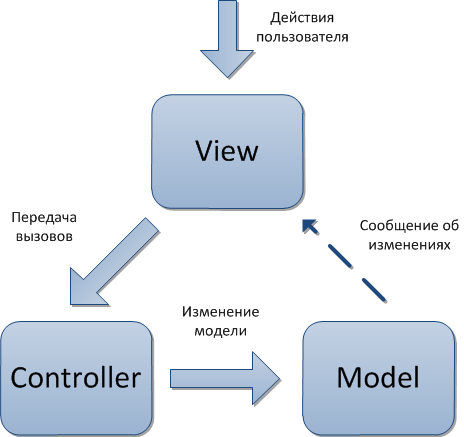
\includegraphics[scale=1]{mvc.png}  
  \caption{ Схема архитектуры MVC. }
  \label{fig:domain:manual_structure:credit_net}
\end{figure}

Таким образом, разбиение на уровни является основным преимуществом использования архитектуры MVC. Её применение будет реализовано на серверной стороне.

% 2 стр

\subsection{Клиентская архитектура приложения Redux}
\label{sub:domain:learning_complexity}

Со стечением времени, архитектура MVC ~\cite{mvc} стала слишком громоздкой и её использование во многих веб-приложениях ориентированных, как клиентское приложение становится уже не целесообразно. На её основе начали создаваться улучшенные виды архитектуры и одна из них является Redux.

Redux ~\cite{redux} может быть описан тремя фундаментальными принципами:
 
\begin{itemize}
  \item единственный источник правды. Состояние всего приложения сохраняется в дереве объектов одного хранилища. Это дает возможность создавать универсальные приложения. Состояние на сервере может быть сериализовано и отправлено на клиент без особых трудностей;
  \item состояние только для чтения. Единственный способ изменить состояние – это применить действие – объект, который описывает, что должно случится;
  \item мутации написаны как простые функции. Для определения того, как дерево состояния будет трансформировано действиями, необходимо писать чистые Reducer-функции. Reducer – функции, которые берут предыдущее состояние и действие и возвращает обновленное состояние. Чистая функция – это функция, которая является детерминированной и не обладает побочными эффектами;
\end{itemize}

\begin{figure}[ht]
\centering
  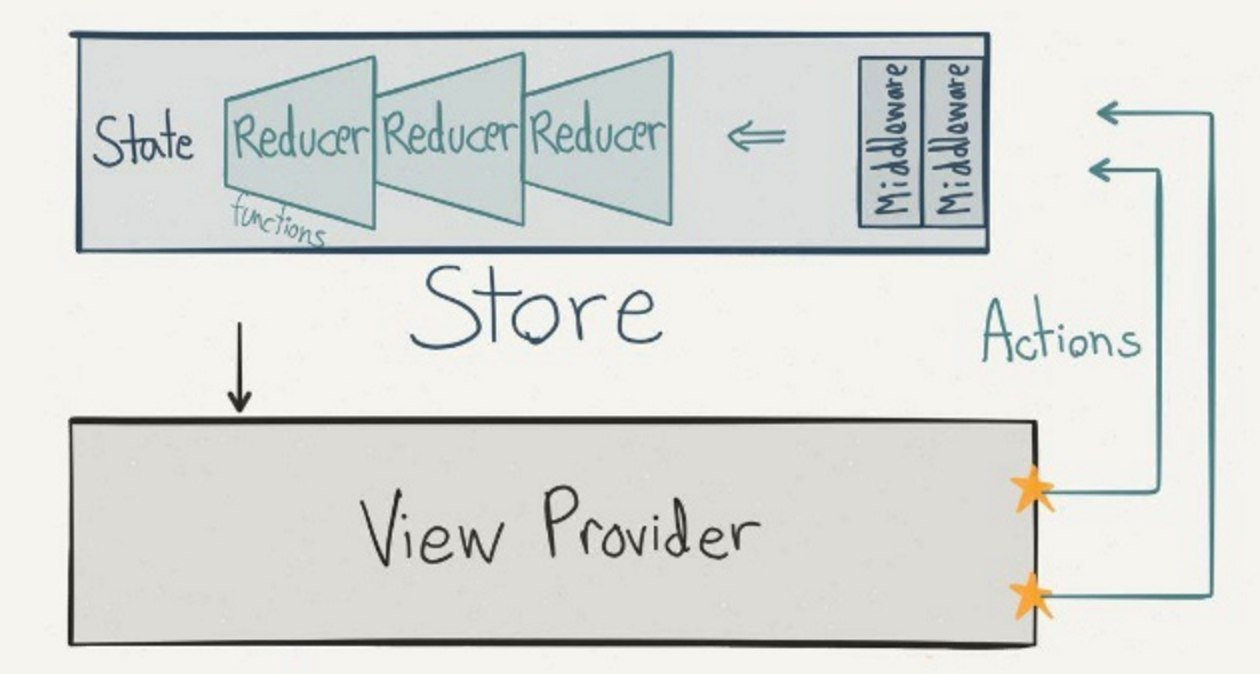
\includegraphics[scale=0.3]{redux.jpg}  
  \caption{ Схема архитектуры Redux. }
  \label{fig:domain:manual_structure:credit_redux}
\end{figure}

На рисунке~\ref{fig:domain:manual_structure:credit_redux}. показана основная схема архитектуры. Разберемся с основными её частями.

Действия (Actions) - это структура, которая передает данные из вашего приложения в хранилище. Они являются единственными источниками информации для хранилища.

Редьюсер (reducer) - это чистая функция, которая принимает предыдущее состояние и действие (state и action ~\cite{redux_framework}) и возвращает следующее состояние (новую версию предыдущего).

Хранилище (Store) - это объект, который соединяет эти части вместе. Хранилище берет на себя следующие задачи:
\begin{itemize}
  \item содержит состояние приложения (application state);
  \item предоставляет доступ к состоянию с помощью getState();
  \item предоставляет возможность обновления состояния с помощью встроенной функции dispatch(action);
  \item регистрирует слушатели (listeners) c помощью subscribe(listener).
\end{itemize}

Таким образом, единственный Store и использование чистых функций является основным преимуществом использования архитектуры Redux.

%Указание что это NP трудная задача (0.5)
%Табличка с оценкой количества сетей в зависимости от числа переменных (для устрашения) (0.2)

\subsection{Платформа Node.js}
\label{sub:domain:mdl_principle}
Node.js ~\cite{node_js} является серверной технологией, которая основана на разработанном компанией Google JavaScript-движке V8 ~\cite{V8}. Это масштабируемая система, поддерживающая не программные потоки или отдельные процессы, а асинхронный ввод-вывод, управляемый событиями. Она идеально подходит для веб-приложений, которые не выполняют сложных вычислений, но к которым происходят частые обращения.

При использовании обычного веб-сервера, например Apache ~\cite{apache}, при каждом запросе веб-ресурса для обслуживания этого запроса сервер создает отдельный программный поток или вызывает новый процесс. Даже если сервер реагирует на запросы достаточно быстро, а после удовлетворения запроса все приводит в порядок, при таком подходе задействуется множество ресурсов. В результате у наиболее популярных веб-приложений возникают предпосылки для серьезных проблем производительности.

В отличие от этого Node не создает новый программный поток или процесс для каждого запроса, а прослушивает конкретные события, и когда эти события происходят, соответствующим образом на них реагирует. Node не блокирует никаких запросов, дожидаясь завершения действий, инициируемых событием, а сами события обрабатываются в относительно простом цикле обработки событий по принципу «первым пришел — первым обслужен».
Node-приложения создаются с помощью языка JavaScript ~\cite{js}(или альтернативных языков, компилирующихся в JavaScript), который ничем не отличается от языка, применяемого в приложениях на стороне клиента. Однако в отличие от языка JavaScript, используемого в браузере, для Node нужно создать среду разработки. Node можно установить на платформе Unix/Linux, Mac OS или Windows.

Рассмотрим работу обычного веб-сервера, например Apache. Apache поддерживает две модели мультипроцессорной обработки (Multiprocessing Model, MPM) поступающих запросов. В первой для каждого запроса выделяется отдельный процесс, продолжающийся до тех пор, пока запрос не будет обслужен, во второй для каждого запроса выделяется отдельный программный поток.

В первой MPM-модели, известной как модель prefork, может создаваться столько дочерних процессов, сколько указано в конфигурационном файле Apache. Преимущество создания отдельного процесса состоит в том, что приложения, к которым обращаются посредством запроса, например PHP-приложения, не обязательно должны быть многопоточными. Недостаток заключается в том, что каждый процесс расходует память, и эта модель характеризуется неважной масштабируемостью.

Во второй MPM-модели, известной как модель worker, реализуется гибридная схема процесс-поток, когда каждый поступающий запрос обрабатывается с помощью нового программного потока. С точки зрения расхода памяти этот подход более эффективен, но он требует, чтобы все приложения были многопоточными (то есть были безопасными в отношении потоков). Хотя популярный язык создания веб-приложений PHP теперь безопасен в отношении потоков, нет никаких гарантий, что множество различных библиотек, используемых с интерпретатором этого языка, также безопасно в отношении потоков.

Независимо от используемой модели, запросы обрабатываются в параллельном режиме. Если к веб-приложению в одно и то же время обращается пять человек и сервер имеет соответствующую настройку, все пять запросов обрабатываются одновременно.

В Node все происходит по-другому. При запуске Node-приложения создается единственный программный поток. Node-приложение выполняется в этом потоке в ожидании, что некое приложение сделает запрос. Когда Node-приложение получает запрос, никакие другие запросы не обрабатываются до тех пор, пока не завершится обработка текущего запроса.

Все это кажется не слишком эффективным, если бы не то обстоятельство, что Node работает в асинхронном режиме, используя цикл обработки событий и функции обратного вызова. Цикл обработки событий просто опрашивает конкретные события и в нужное время вызывает обработчики событий. В Node таким обработчиком событий является функция обратного вызова.

В отличие от других однопоточных приложений, когда к Node-приложению делается запрос, оно должно, в свою очередь, запросить какие-то ресурсы (например, обратиться к базе данных или получить доступ к файлу). В этом случае Node инициирует запрос, но не ожидает ответа на этот запрос. Вместо этого запросу назначается некая функция обратного вызова. Когда запрошенное будет готово (или завершено), генерируется событие, активизирующее соответствующую функцию обратного вызова, призванную что-то сделать либо с результатом запрошенного действия, либо с запрошенными ресурсами.

Если пять человек обращаются к Node-приложению в одно и то же время и приложению нужно обратиться к ресурсам из файла, для каждого запроса Node назначает свою функцию обратного вызова событию ответа. Когда для каждого из них ресурс становится доступен, вызывается нужная функция обратного вызова, и запрос удовлетворяется. В промежутке Node-приложение может обрабатывать другие запросы либо для того же приложения, либо для какого-нибудь  другого.

% MDL (2-3)


\subsection{Преимущества NoSQL по сравнению с реляционными СУБД}
\label{sub:domain:k2_algo}
NoSQL ~\cite{nosql} – ряд подходов, направленных на реализацию хранилищ баз данных, имеющих существенные отличия от моделей, используемых в традиционных реляционных СУБД с доступом к данным средствами языка SQL. Применяется к базам данных, в которых делается попытка решить проблемы масштабируемости и доступности за счёт атомарности и согласованности данных.

В реляционной модели база состоит из таблиц, которые состоят из строк и колонок. У каждой колонки есть свой тип данных (строка, число, логическое значение, дата, текст, бинарный блоб). Все строки однотипны.
Обычно каждый вид объектов хранится в отдельной таблице. Обычно у каждого объекта есть уникальный идентификатор. Идентификатор может быть как условным, то есть просто числом, так и вытекающим из предметной области.

Серверы реляционных БД обеспечивают стандартные операторы доступа к данным в таблицах, такие как SELECT, INSERT, UPDATE и DELETE. Разные серверы предоставляют также некоторые дополнительные операторы. Извлекать данные из таблиц можно по множеству различных критериев.

NoSQL – это отход от реляционной модели в пользу более специфических моделей данных. Например, традиционно успешными NoSQL-системами являются системы хранения пар “ключ-значение”, документные хранилища и графовые базы данных.

У NoSQL обычно перечисляют следующие достоинства:
\begin{itemize}
  \item масштабируемость. Горизонтальное масштабирование существующих традиционных СУБД обычно является трудоемкой, дорогостоящей и эффективной только до определенного уровня задачей. В то же время многие NoSQL-решения проектировались исходя из необходимости масштабироваться горизонтально и делать это «на лету». Поэтому эта процедура обычно проще и прозрачнее в NoSQL, чем в РСУБД;
  \item производительность БД на одном узле, а не в кластере также является немаловажным параметром. Для многих задач такие свойства традиционных СУБД, как транзакционность, изолированность изменений, надежность в пределах одного узла или даже сама реляционная модель, не всегда нужны в полном объеме. Поэтому отказ от этих свойств (всех или некоторых) позволяет NoSQL иногда добиваться большей производительности на одном узле, чем традиционным решениям;
  \item надежная работа в условиях, когда отказ железа или сетевая недоступность – обычное дело, является одним из свойств многих решений NoSQL. Основной способ ее обеспечения – это репликация. Сама по себе репликация отнюдь не является уникальной особенностью NoSQL, но здесь, как и при масштабировании, важную роль играют эффективность и легкость внесения изменений в существующую инсталляцию. Переход БД к работе в режиме репликации – это простая задача для большинства NoSQL-решений;
  \item простота разработки и администрирования – также важный аргумент в пользу NoSQL-технологий. Целый ряд задач, связанных с масштабированием и репликацией, представляющих значительную сложность и требующих обширной специальной экспертизы на традиционных СУБД, у NoSQL занимает считанные минуты. Задачи установки и настройки, само использование NoSQL-решений обычно существенно проще и менее трудоемки, чем в случае с РСУБД. Поэтому NoSQL-системы стали очевидным выбором для многих проектов, где скорость разработки и внедрения является ключевым фактором.
\end{itemize}

%Оценка апостериорных вероятностей (K2) (2-3)

\subsection{Фреймворк ReactJS}
\label{sub:domain:other_algos}
React.js ~\cite{react_js}— фреймворк для создания интерфейсов от Facebook. React построен на парадигме реактивного программирования. Этот декларативный подход предлагает описывать данные в виде набора утверждений или формул. Изменение одного из параметров ведёт за собой автоматический пересчёт всех зависимостей.Работа с DOM в браузере часто оказывается источником проблем с производительностью. Создатели React решили проблему радикально. Ребята написали реализацию DOM на JavaScript. Фреймворк использует её, чтобы при изменении состояния компонент судить о том, что поменять в реальном DOM и как сделать это эффективно.

\subsection{Cordova}
\label{sub:domain:other_algos2}
Apache Cordova ~\cite{cordova} — это платформа разработки мобильных приложений с открытым исходным кодом. Она позволяет использовать стандартные веб-технологии, такие как HTML5, CSS3 и JavaScript для кросс платформенной разработки, избегая родного языка разработки для каждой из мобильных платформ. Приложения выполняются внутри обертки нацеленной на каждую платформу и полагаются на стандартные API для доступа к датчикам устройства, данным и состоянию сети.

Приложения Cordova полагаются на общий файл config.xml, который содержит информацию о приложении и определяет параметры, влияющие на то как приложенеи работает, такие как, реагирует ли оно на изменение ориентации устройства. Этот файл соответствует спецификации W3C Упакованные веб-приложения, или widget.

Само приложение реализована как веб-страницы, по умолчанию локальный файл под названием index.html, который ссылается на любой CSS, JavaScript, изображения, файлы мультимедиа или другие ресурсы необходимы для его запуска. Приложение выполняет как WebView в пределах оболочки приложения, которую вы распространяете в магазины приложений.

WebView с поддержкой Cordova может представлять приложения и полностью его пользовательский интерфейс. На некоторых платформах она также может быть компонентом в больших, гибридные приложения, который объединяют WebView с другими компонентами приложения. (Подробную информацию см. в разделе "Интеграция WebViews".)

Интерфейс плагина доступен для Cordova и других компоненты, для взаимодействия друг с другом. Это позволяет вызывать код на языке платформы из JavaScript. В идеале на нескольких платформах устройств согласуются JavaScript API, чтобы этот машинный код. Начиная с версии 3.0 плагины предоставляют привязки к стандартным API интерфейсам устройства. Сторонние плагины предоставляют дополнительные привязки для функции не обязательно доступных на всех платформах.

\subsection{Безопасность приложения}
\label{sub:domain:other_algos3}
Безопасность является важнейшей частью веб-ориентированного приложения. Под безопасностью приложения следует понимать такие условия, когда действие внешних и внутренних факторов не влечет негативных действий по отношению к данному приложению.
Для обеспечения защиты приложения и данных используются следующие подходы, реализованные в платформе Node.JS:
\begin{itemize}
  \item защита от CSRF-атак (cross-site request forgery, межсайтовая подделка запроса), при которых данные пользователя могут быть переданы на другой сайт (например, сайт злоумышленника или сайт платежной системы) для совершения некой вредоносной операции;
  \item аутентификация пользователей, позволяющая идентифицировать пользователя и гарантировать эту идентификацию;
  \item авторизация пользователей, которая позволяет разграничивать права доступа пользователей к ресурсам;
  \item конфиденциальность пользователей, которая гарантирует невозможность получения данных пользователя третьими лицами;
  \item обеспечение целостности передаваемых данных и гарантия невозможности их подмены злоумышленником;
  \item щифрование трафика, передаваемого по сети;
  \item обязательное экранирование всех входных данных (для избегания нанесения ущерба данным пользователя). Стоит всегда иметь в виду, что любые данные, полученные от пользователя, могут являться вредоносными;
  \item защита файлов cookie;
\end{itemize}

% Ограничения других методов построения (упорядоченность нод, ) (2)

\subsection{Обзор существующих программ} % (fold)
\label{sub:domain:existing_programs}
Существует много приложений, в основе работы которых лежит инструменты личного мониторинга здоровья. В основе этих инструментов может лежать как и веб-ориентированное приложения, так и десктопные приложения. Рассмотрим наиболее популярные из них.

Приняв во внимание тему дипломного проекта, наибольший интерес в существуем ПО будет представлять функциональность возможность работы с большим количеством данных.
Ниже рассматриваются некоторые из программ.

\subsubsection{МедАрхив }(\url{https://www.medarhiv.ru/}) 
Проект организован с целью информационной поддержки медицинского обслуживания. Медархив - это web-площадка для обмена медицинской информацией между врачами и медицинскими учреждениями, с одной стороны, и пациентами, с другой. Работа Медархива ориентирована на потребности тех, кто лечит, и тех, кто лечится.

Пациент и врач могут взаимодействовать через Медархив почти так же, как реальном мире. Пациент рассказывает о проблеме, врач дает рекомендации, отправляет на обследование, ставит диагноз. Личная медицинская информация, включая консультации врача, электронную медицинскую карту, надежно и конфиденциально хранится в архиве пациента.
Достоинства:
\begin{itemize}
  \item удобная панель навигации. Она позволяет быстро найти необходимый пункт;
  \item быстрый просмотр сведений. Возможность просматривать информацию о себе, о врачах;
  \item организация расписания. Позволяет не только смотреть за расписанием определенных врачей. Но и организовывать собственное расписание;
  \item онлайн консультация, а также онлайн запись на прием к врачу.
\end{itemize}
Недостатки:
\begin{itemize}
  \item отсутсивие кроссплатформенности;
  \item недоступность утилит для автоматизации создания встреч;
  \item нет возможности следить за своим ребенком. Нужно создавать отдельный аккаунт;
\end{itemize}
\begin{figure}[ht]
\centering
  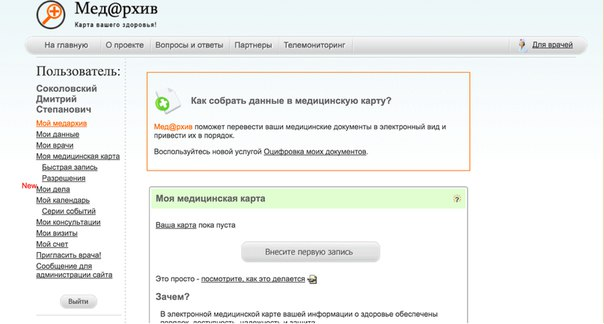
\includegraphics[scale=0.7]{medAr.jpg}  
  \caption{ Главная страница пациента приложения МедАрхив. }
  \label{fig:domain:manual_structure:credit_med}
\end{figure}


\subsubsection{HealthKit}(\url{https://developer.apple.com/healthkit/}) 
Приложение под продукцию Apple. На первый взгляд в нём сложно разобраться. HealthKit — это платформа, которая будет собирать информацию о вашем состоянии не только на основе датчиков одного трекера, а отовсюду, откуда это только возможно. Из приложений, которые установлены на вашем iPhone и iPad, из фитнес-устройств. Таким образом HealthKit будет выдавать полную картинку о вашем состоянии. Мало того, в iOS 8 приложения смогут обмениваться информацией с HealthKit , чтобы сделать тренировки эффективнее или подкоректировать диету.
Достоинства:
\begin{itemize}
  \item большие возможности кастомизации;
  \item есть возможность анализировать график анализа жизненных покозателей;
  \item удобный интерфейс пользователя;
\end{itemize}
Недостатки:
\begin{itemize}
  \item избыточная сложность;
  \item не кроссплатформенность;
  \item нет возможность расшарить данные врачу или медцентру;
\end{itemize}

\begin{figure}[ht]
\centering
  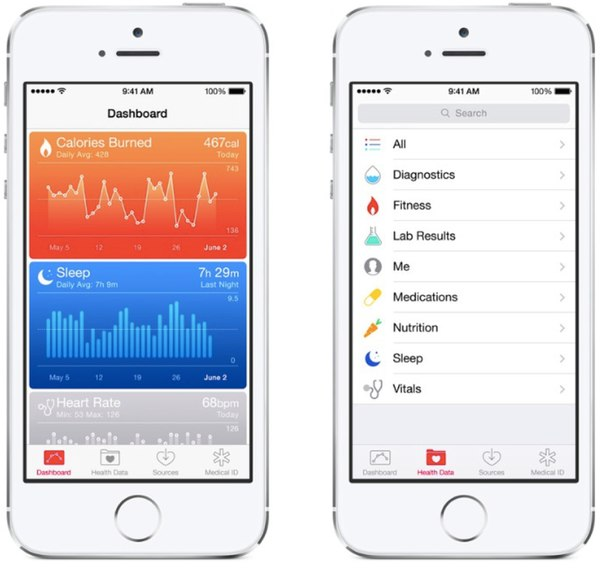
\includegraphics[scale=0.7]{healthkit.jpg}  
  \caption{ Приложение HealthKit. }
  \label{fig:domain:manual_structure:credit_healthkit}
\end{figure}

\subsubsection{OnDoc }
\label{sub:domain:existing_programs:genie}

OnDoc - новый бесплатный веб-сервис + мобильное приложение (iOS, Android) для хранения персональных медицинских данных. Вы можете добавлять записи о результатах посещения врача и проведенных обследованиях. Тут же можно записаться на прием в любую из 4 тыс. клиник-партнеров сервиса. После приема в партнерских клиниках информация об обследовании, диагнозе и лечении появляются в профиле автоматически. Можно предоставить онлайн доступ другому врачу к своим данным. Также приложение может напоминать о приеме лекарств и дозировке, выдавать персональные рекомендации по снижению риска возможных заболеваний. Разработчики утверждают, что вся информация в сервисе хранится в зашифрованном виде в соответствии с 152 ФЗ <<О персональных данных>>.

\begin{itemize}
  \item легкий интерфейс;
  \item кроссплатформенность;
  \item возможность выбора нескольких клиник или медцентров;
  \item возможность организовывать прием медицинских препаратов;
  \item возможность анализировать состояние здоровья за определенный срок;
\end{itemize}
Недостатки:
\begin{itemize}
  \item отсутсвует календарь;
  \item нет полноценного функционала импорта/экспорта;
  \item нет доступа к полноценной кастомизации;
\end{itemize}


\subsection{Обоснование выбора языка и среды разработки} % (fold)
\label{sub:domain:existing_language}
\subsubsection{Язык разработки }

Исходные коды программного средства должны быть реализованы на языке программирования JavaScript. Обусловлен этот выбор следующими критериями:

\begin{itemize}
  \item язык JavaScript - язык программирования с динамической типизацией, позволяющей писать более краткий и лаконичный код;
  \item встроенная поддержка юникода в строках;
  \item JavaScript не вынуждает писать код в определенном стиле и парадигме;

  \item автоматическая сборка мусора;
  \item кроссплатформенность, подразумевающая, что программное средство, написанное на языке программирования JavaScript, будет функционировать одинаково, вне зависимости от операционной системы и браузера;
  \item JavaScript является мультипарадигменным языком, что позволяет использовать различные решения, лучше подходящие для данной задачи;

  \item большое количество библиотек;
  \item возможность использовать JavaScript как на сервере, так и на клиенте;
  \item широкая распространенность JavaScript, что позволит разобраться в коде большему количеству разработчиков без предварительной подготовки;
\end{itemize}

В качестве интегрированной среды разработки программного средства должно быть использовано программное обеспечение JetBrains WebStorm ~\cite{webstorm}, в силу следующих качеств, присущих ему:
\begin{itemize}
  \item возможность работы под различными операционными системами: OS Windows, Linux, Mac OS X;
  \item встроенный отладчик для языка платформы Node.js;
  \item поддержка систем контроля версий: общий пользовательский интерфейс для Mercrurial, Git, Subversion, Perforce и CVS с поддержкой списков изменений и слияния;

  \item статический анализ кода, подсветка синтаксиса и ошибок;
  \item навигация по проекту и исходному коду: отображение файловой структуры проекта, быстрый переход между файлами, классами, методами и использованиями методов;
\end{itemize}

\subsubsection{Выбор платформы разработки }

 Серверная сторона приложения разработана с использованием платформы Node.JS.
Node.js — программная платформа, основанная на движке V8 (транслирующем JavaScript в машинный код), превращающая JavaScript из узкоспециализированного языка в язык общего назначения. Node.js добавляет возможность JavaScript взаимодействовать с устройствами ввода-вывода через свой API (написанный на C++), подключать другие внешние библиотеки, написанные на разных языках, обеспечивая вызовы к ним из JavaScript-кода. Node.js применяется преимущественно на сервере, выполняя роль веб-сервера, но есть возможность разрабатывать на Node.js и десктопные оконные приложения (при помощи NW.js, AppJS или Electron для Linux, Windows и Mac OS) и даже программировать микроконтроллеры (например, tessel и espruino). В основе Node.js лежит событийно-ориентированное и асинхронное (или реактивное) программирование с неблокирующим вводом/выводом.

\subsubsection{Выбор СУБД }

 MongoDb ~\cite{mongodb} — это документо-ориентированная база данных. Т.е. каждая запись это документ, без жестко заданной схемы, который может содержать вложенные документы.

MongoDb ~\cite{mongodb} хороша высокой скоростью записи/чтения, масштабированностью, но опять же сохранность и целостность данных не так хороша. Так, например, в Монго есть отличная реализация репликации, которая довольно легко устанавливается и настраивается или же шардинг (возможность разнести данные по нескольким серверам), который тоже довольно прост в установке. В комплексе, можно получить систему распределенных вычислений с высокой отказоустойчивостью.

MongoDb — использует JSON нотацию для хранения и управления документами, а также свой достаточно удобный язык запросов.

Основные возможности данной СУБД:
\begin{itemize}
  \item документо-ориентированное хранилище (простая и мощная JSON-подобная схема данных);
  \item достаточно гибкий язык для формирования запросов;
  \item динамические запросы;
  \item полная поддержка индексов;
  \item профилирование запросов;
  \item быстрые обновления «на месте»;
  \item эффективное хранение двоичных данных больших объёмов, напр., фото и видео;
  \item журналирование операций, модифицирующих данные в БД;
  \item поддержка отказоустойчивости и масштабируемости: асинхронная репликация, набор реплик и шардинг
Может работать в соответствии с парадигмой MapReduce;
\end{itemize}

\subsubsection{ORM Mongoose }

 В данном проекте будет использоваться Mongoose.
Mongoose — это библиотека Node.js, которая предоставляет возможность объектно-реляционного отображения, схожего со знакомым интерфейсом внутри Node.js. Mongoose переводит данные в базу данных объектов JavaScript для дальнейшего их использования вашим приложением


\subsection{Постановка задачи } % (fold)
\label{sub:domain:existing_tasked}
Таким образом в результате обзора аналогов и их недостатков была составлена укрупненная спецификация требований.

Цели проекта:
\begin{itemize}
  \item предоставить пациенту следить за своим здоровьем;
\end{itemize}
Задачи проекта:
\begin{itemize}
  \item упростить взаимодействие пациентов и медучреждений;
\end{itemize}
Аудитория проекта:
\begin{itemize}
  \item семейные люди;
  \item одинокие люди;
\end{itemize}
Функциональность проекта:
\begin{itemize}
  \item ведение базы данных о пациентах;
  \item система авторизации в приложении;
  \item просмотр списка заключений от медучреждений;
  \item возможность создавать вручную заключения полученные от медучереждений;
  \item возможность сканирование фотографии заключения медучреждения;
  \item возможность экспортирования списка или одного заключения от медучреждения;
\end{itemize}

Требования к реализации:
\begin{itemize}
  \item удобный пользовательский интерфейс;
  \item высокая скорость работы мобильного приложения;
  \item отказоустойчивость архитектуры;
  \item работа на современных мобильных операционных системах (iOS, Android);
\end{itemize}


\lstset{style=fsharpstyle}

\section{Моделирование предметной области} 
\label{sec:practice:technology_used}


\subsection{Use-case диаграмма }
\label{sub:practice:microsoft_net}

Use-case diagram в UML – диаграмма, отражающая отношения между актёрами и прецедентами и являющаяся составной частью модели прецедентов, позволяющей описать систему на концептуальном уровне.

Прецедент – возможность моделируемой системы (часть её функциональности), благодаря которой пользователь может получить конкретный, измеримый и нужный ему результат. Прецедент соответствует отдельному сервису системы, определяет один из вариантов её использования и описывает типичный способ взаимодействия пользователя с системой. Варианты использования обычно применяются для спецификации внешних требований к системе. Основное назначение диаграммы – описание функциональности и поведения, позволяющее заказчику, конечному пользователю и разработчику совместно обсуждать проектируемую или существующую систему.

При моделировании системы с помощью диаграммы прецедентов системный аналитик стремится:
\begin{itemize}
  \item чётко отделить систему от её окружения;
  \item определить действующих лиц (актёров), их взаимодействие с системой и ожидаемый функционал системы;
  \item определить в глоссарии предметной области понятия, относящиеся к детальному описанию функционала системы (то есть, прецедентов).
\end{itemize}

Работа над диаграммой может начаться с текстового описания, полученного при работе с заказчиком. При этом нефункциональные требования (например, конкретный язык или система программирования) при составлении модели прецедентов опускаются (для них составляется другой документ).
Для отражения модели прецедентов на диаграмме используются:

\begin{itemize}
  \item рамки системы – прямоугольник с названием в верхней части и эллипсами (прецедентами) внутри. Часто может быть опущен без потери полезной информации;
  \item актёр обозначает набор ролей пользователя (понимается в широком смысле: человек, внешняя сущность, класс, другая система), взаимодействующего с некоторой сущностью (системой, подсистемой, классом). Актёры не могут быть связаны друг с другом (за исключением отношений генерализации/наследования);
  \item  прецедент – эллипс с надписью, обозначающий выполняемые системой действия (могут включать возможные варианты), приводящие к наблюдаемым актёрами результатам. Надпись может быть именем или описанием (с точки зрения актёров) того, <<что>> делает система (а не <<как>>).
\end{itemize}

Имя прецедента связано с непрерываемым (атомарным) сценарием – конкретной последовательностью действий, иллюстрирующей поведение. В ходе сценария актёры обмениваются с системой сообщениями. Сценарий  может быть приведён на диаграмме прецедентов в виде UML-комментария. С одним прецедентом может быть связано несколько различных сценариев.

Для представления функциональной модели была выбрана диаграмма вариантов использования - UML, которая отражает отношения между актерами и прецедентами и позволяет описать систему на концептуальном уровне. Прецедент соответствует отдельному сервису системы, определяет один из вариантов её использования и описывает типичный  способо взаимодействия пользователй с системой. UML предназначен для определения, визуализации, проектирования и документирования программных систем.

\begin{figure}[ht]
\centering
  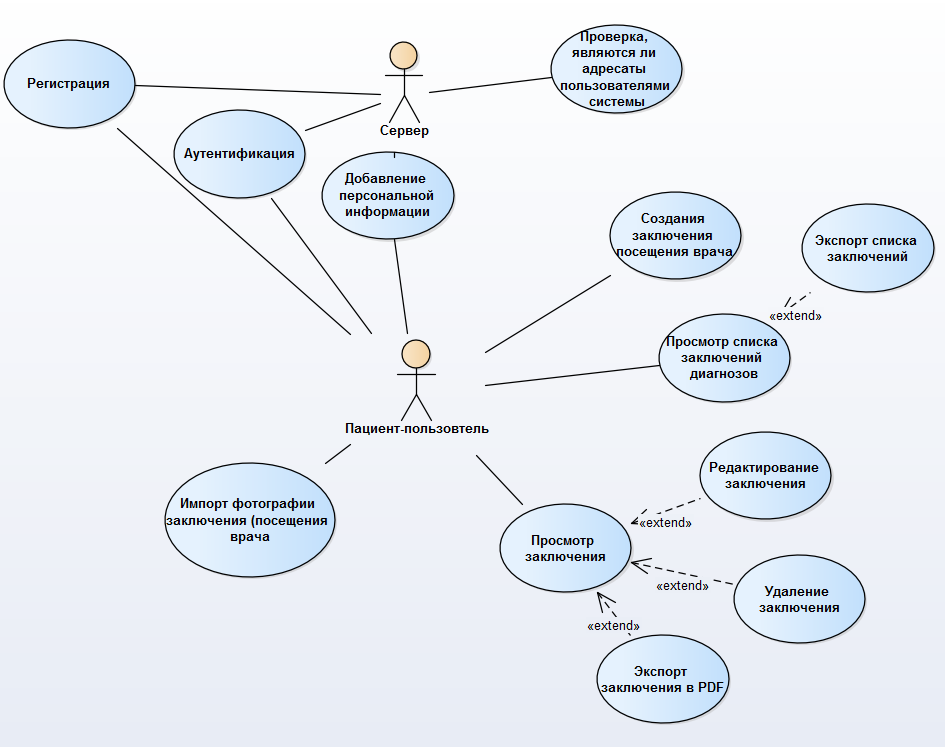
\includegraphics[scale=0.7]{usecase.png}  
  \caption{ Диаграмма вариантов использования }
  \label{fig:domain:manual_structure:credit_usecase}
\end{figure}


\subsection{Спецификация требований }
\label{sub:practice:tab_task}

Исходя из анализа литературы и аналогов, разработанной схемы базы данных, было разработано техническое задание к мобильному программному средству «Органайзер здоровья пациента»: 

\begin{enumerate}
\item cоздание модуля регистрации и авторизации;
\item cоздание модуля для создания и редактирования персональной информации пользователя;
\item cоздание модуля создания и редактирования медицинских карточек (заключение посещения врача):
\begin{enumerate}
\item реализация логики сохранения заключений в БД;
\item реализация логики обновления всех информационных полей заключений;
\end{enumerate}
\item создание модуля работы с PDF экспортом:
\begin{enumerate}
\item реализация возможности экспортирования всех медицинских заключений;
\item реализация возможности экспортирования выбранного медицинского заключения;
\item реализация логики формирования документа;
\end{enumerate}
\item создание модуля обработки изображений:
\begin{enumerate}
\item реализация возможности предварительного просмотра полученного изображения;
\item реализация логики считывания информации с изображения;
\item реализация логики распознавания полученного текста с изображения;
\item реализация возможности создания заключения, используя полученные данные с изображения;
\end{enumerate}
\item реализация модуля настроек системы:
\begin{enumerate}
\item реализация возможности изменения информации о пользователе;
\item реализация возможности выхода из приложения.
\end{enumerate}
\end{enumerate}


\section{Архитектура программного средства} % (fold)
\label{sec:arch_and_mod}

\subsection{Разработка программного развертывания}
\label{sub:arch_and_mod:graphlib}

Прежде чем приступать к непосредственной реализации программного средства, необходимо определиться с архитектурой коллективной работы с приложением.

Во-первых, необходимо провести анализ необходимой аппаратной конфигурации, на которой будут работать части конечного программного средства, и описать их взаимодействие между собой. Для описания узлов и их связей будем использовать диаграмму развертывания.

\begin{figure}[ht]
\centering
  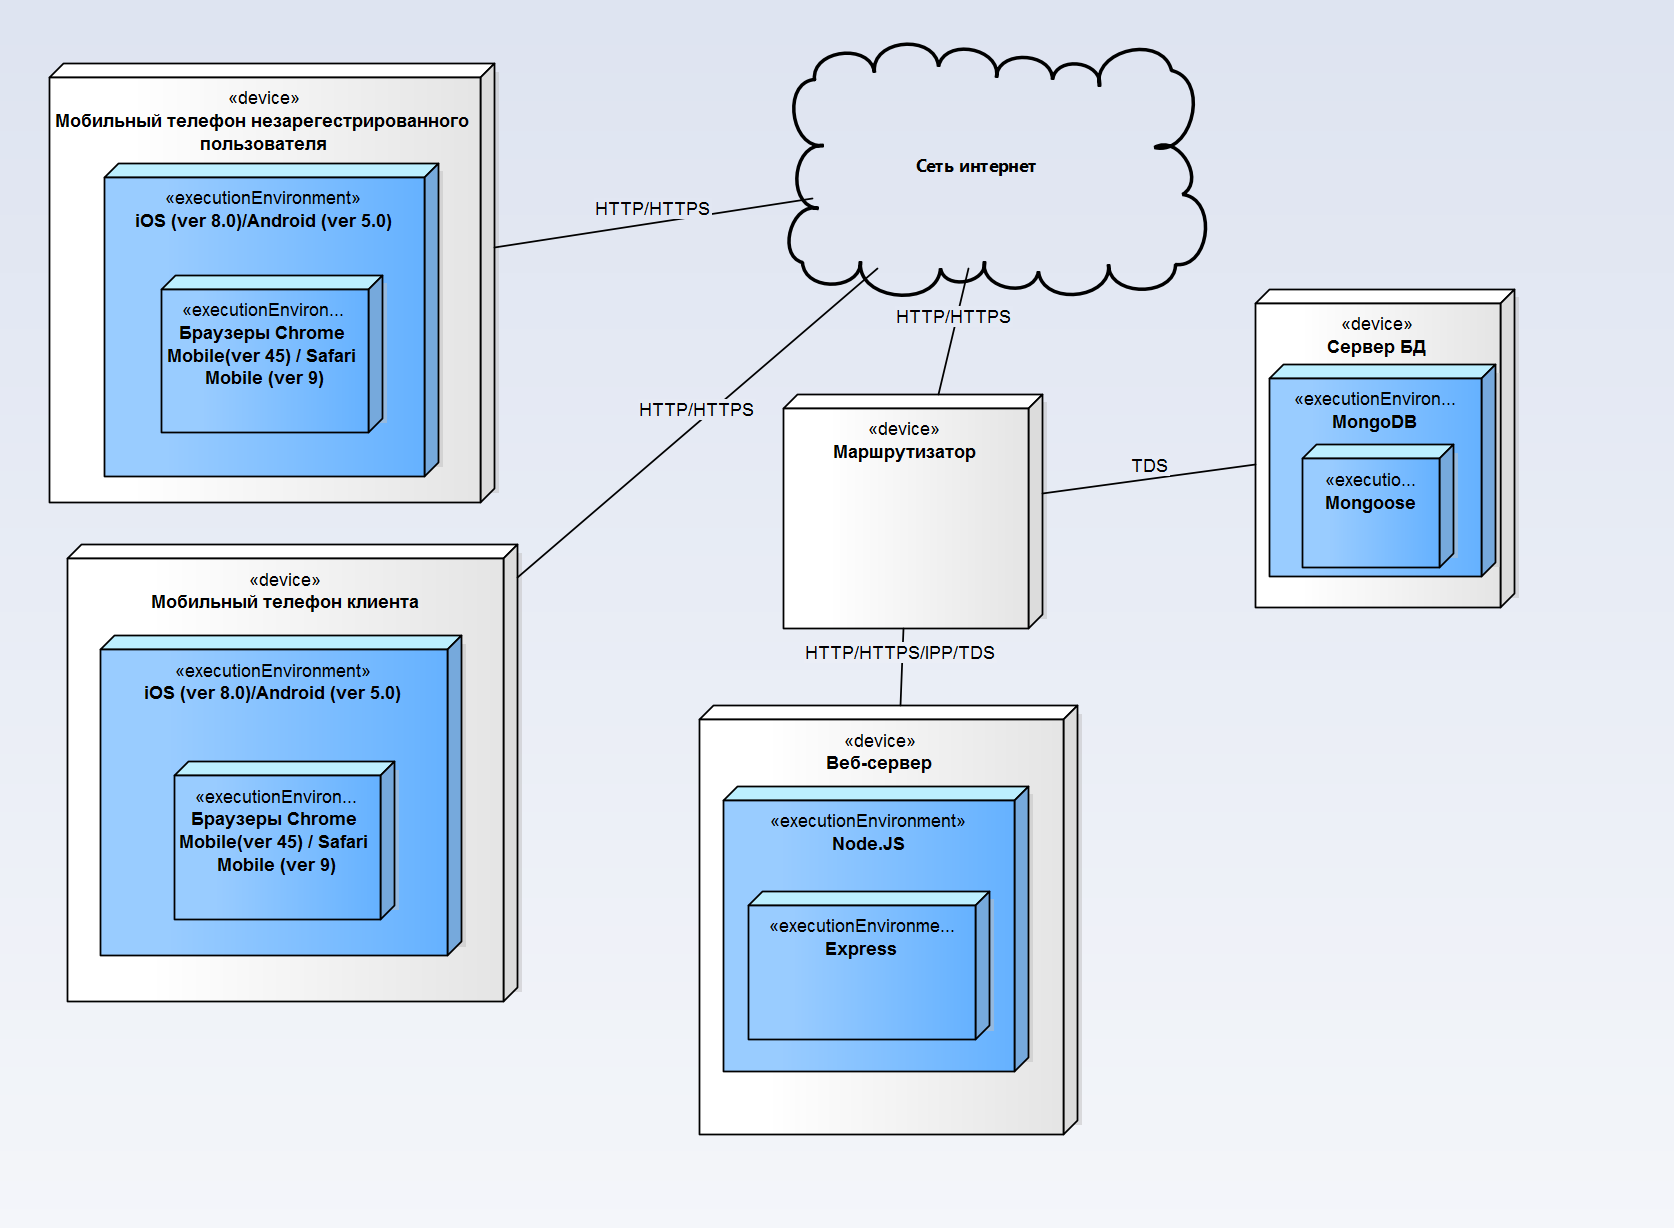
\includegraphics[scale=0.5]{device.png}  
  \caption{Диаграмма развертывания}
  \label{fig:domain:manual_structure:credit_device}
\end{figure}

На основе вышеизображенной диаграммы можно сделать следующие выводы:

\begin{enumerate}
  \item узлы могут располагаться в различных частях мира и взаимодействовать между собой через сеть Интернет;
  \item сервер базы данных поддерживаются в рабочем состоянии отдельно от основного сервера;
  \item клиент, взаимодействует с системой с помощью HTTP/HTTPS.
\end{enumerate}

\subsection{Разработка архитектуры БД }
\label{sub:arch_and_mod:graphlib}

Перед тем, как приступать к процессу разработки, сначала нужно смоделировать базу данных, которая является оcновой будущего приложения. Чтобы база данных не вызывала трудностей при работе с ней, когда будет заполнена информацией, крайне желательно, чтобы она соответствовала трем нормальным формам:
\begin{itemize}
  \item защита от CSRF-атак (cross-site request forgery, межсайтовая подделка запроса), при которых данные пользователя могут быть переданы на другой сайт (например, сайт злоумышленника или сайт платежной системы) для совершения некой вредоносной операции.
  \item Первая нормальная форма. Переменная отношения находится в первой нормальной форме тогда и только тогда, когда в любом допустимом значении отношения каждый его кортеж содержит только одно значение для каждого из атрибутов. 
  \item Вторая нормальная форма. Переменная отношения находится во второй нормальной форме тогда и только тогда, когда она находится в первой нормальной форме, и каждый неключевой атрибут функционально полно зависит от ее потенциального ключа.
  \item Третья нормальная форма. Переменная отношения находится в третьей нормальной форме тогда и только тогда, когда она находится во второй нормальной форме, и отсутствуют транзитивные функциональные зависимости неключевых атрибутов от ключевых.
\end{itemize}

В дипломном проекте будет разрабатываться нереляционная база данных. Делаться это будет путем создания JavaScript объектов, которые в последствии дополняться необходимыми полями, которые будут хранится в базе данных также в виде объектов. Преимущества данного подхода являются: 
\begin{enumerate}
  \item решение проблемы масштабируемости;
  \item решение проблемы доступности;
  \item применение различных типов хранилищ;
  \item возможность создания базы данных без задания схемы;
  \item возможность использования многопроцессорности;
  \item сокращение времени разработки;
  \item скорость и производительность.
\end{enumerate}

\begin{figure}[ht]
\centering
  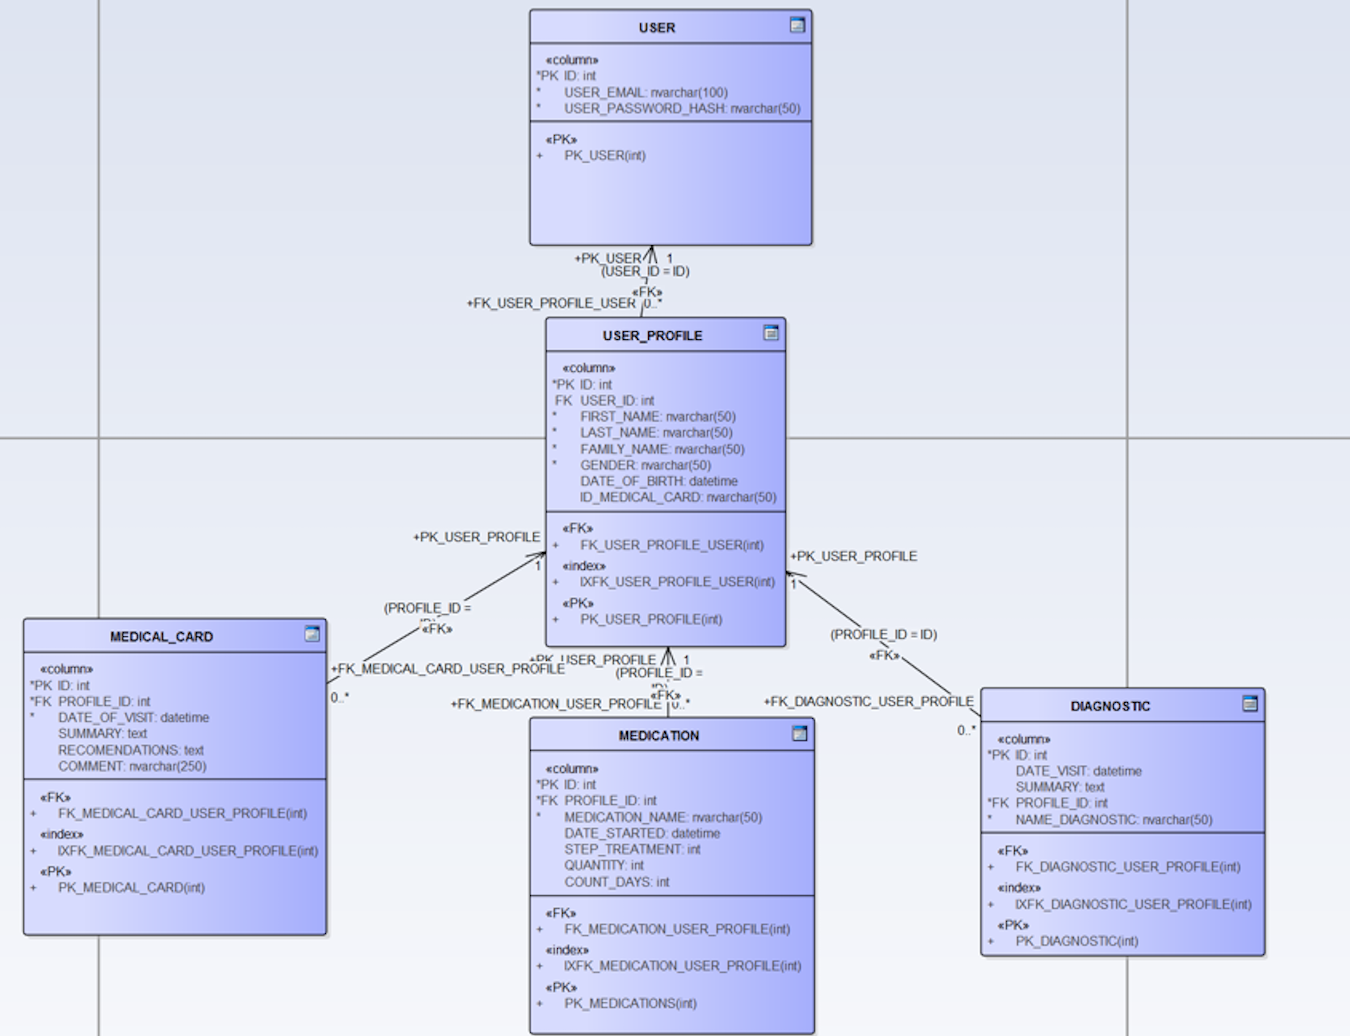
\includegraphics[scale=0.7]{db.png}  
  \caption{Модель базы данных программного средства}
  \label{fig:domain:manual_structure:credit_dbz}
\end{figure}

Схема базы данных разрабатываемого приложения имеет следующий вид, представленный на рисунке~\ref{fig:domain:manual_structure:credit_dbz}. Она состоит из 5 таблиц. Главной таблицей является User. В ней собраны поля, которые необходимы для регистрации и авторизации пользователя. Для заполнение и редактирования самого профиля, есть таблица UserProfile, в которой собраны поля информационного характера о пользователе. Таблицы MedicalCard, Medication и Diagnostic используются для занесении информации о заключениях пациента, различного формата: заключение терапевта, заключение о назначении различных медикаментов и заключение о прохождении различных видов диагностик.

\subsection{Разработка алгоритма ПС }
\label{sub:arch_and_mod:alholib}

\begin{figure}[ht]
\centering
  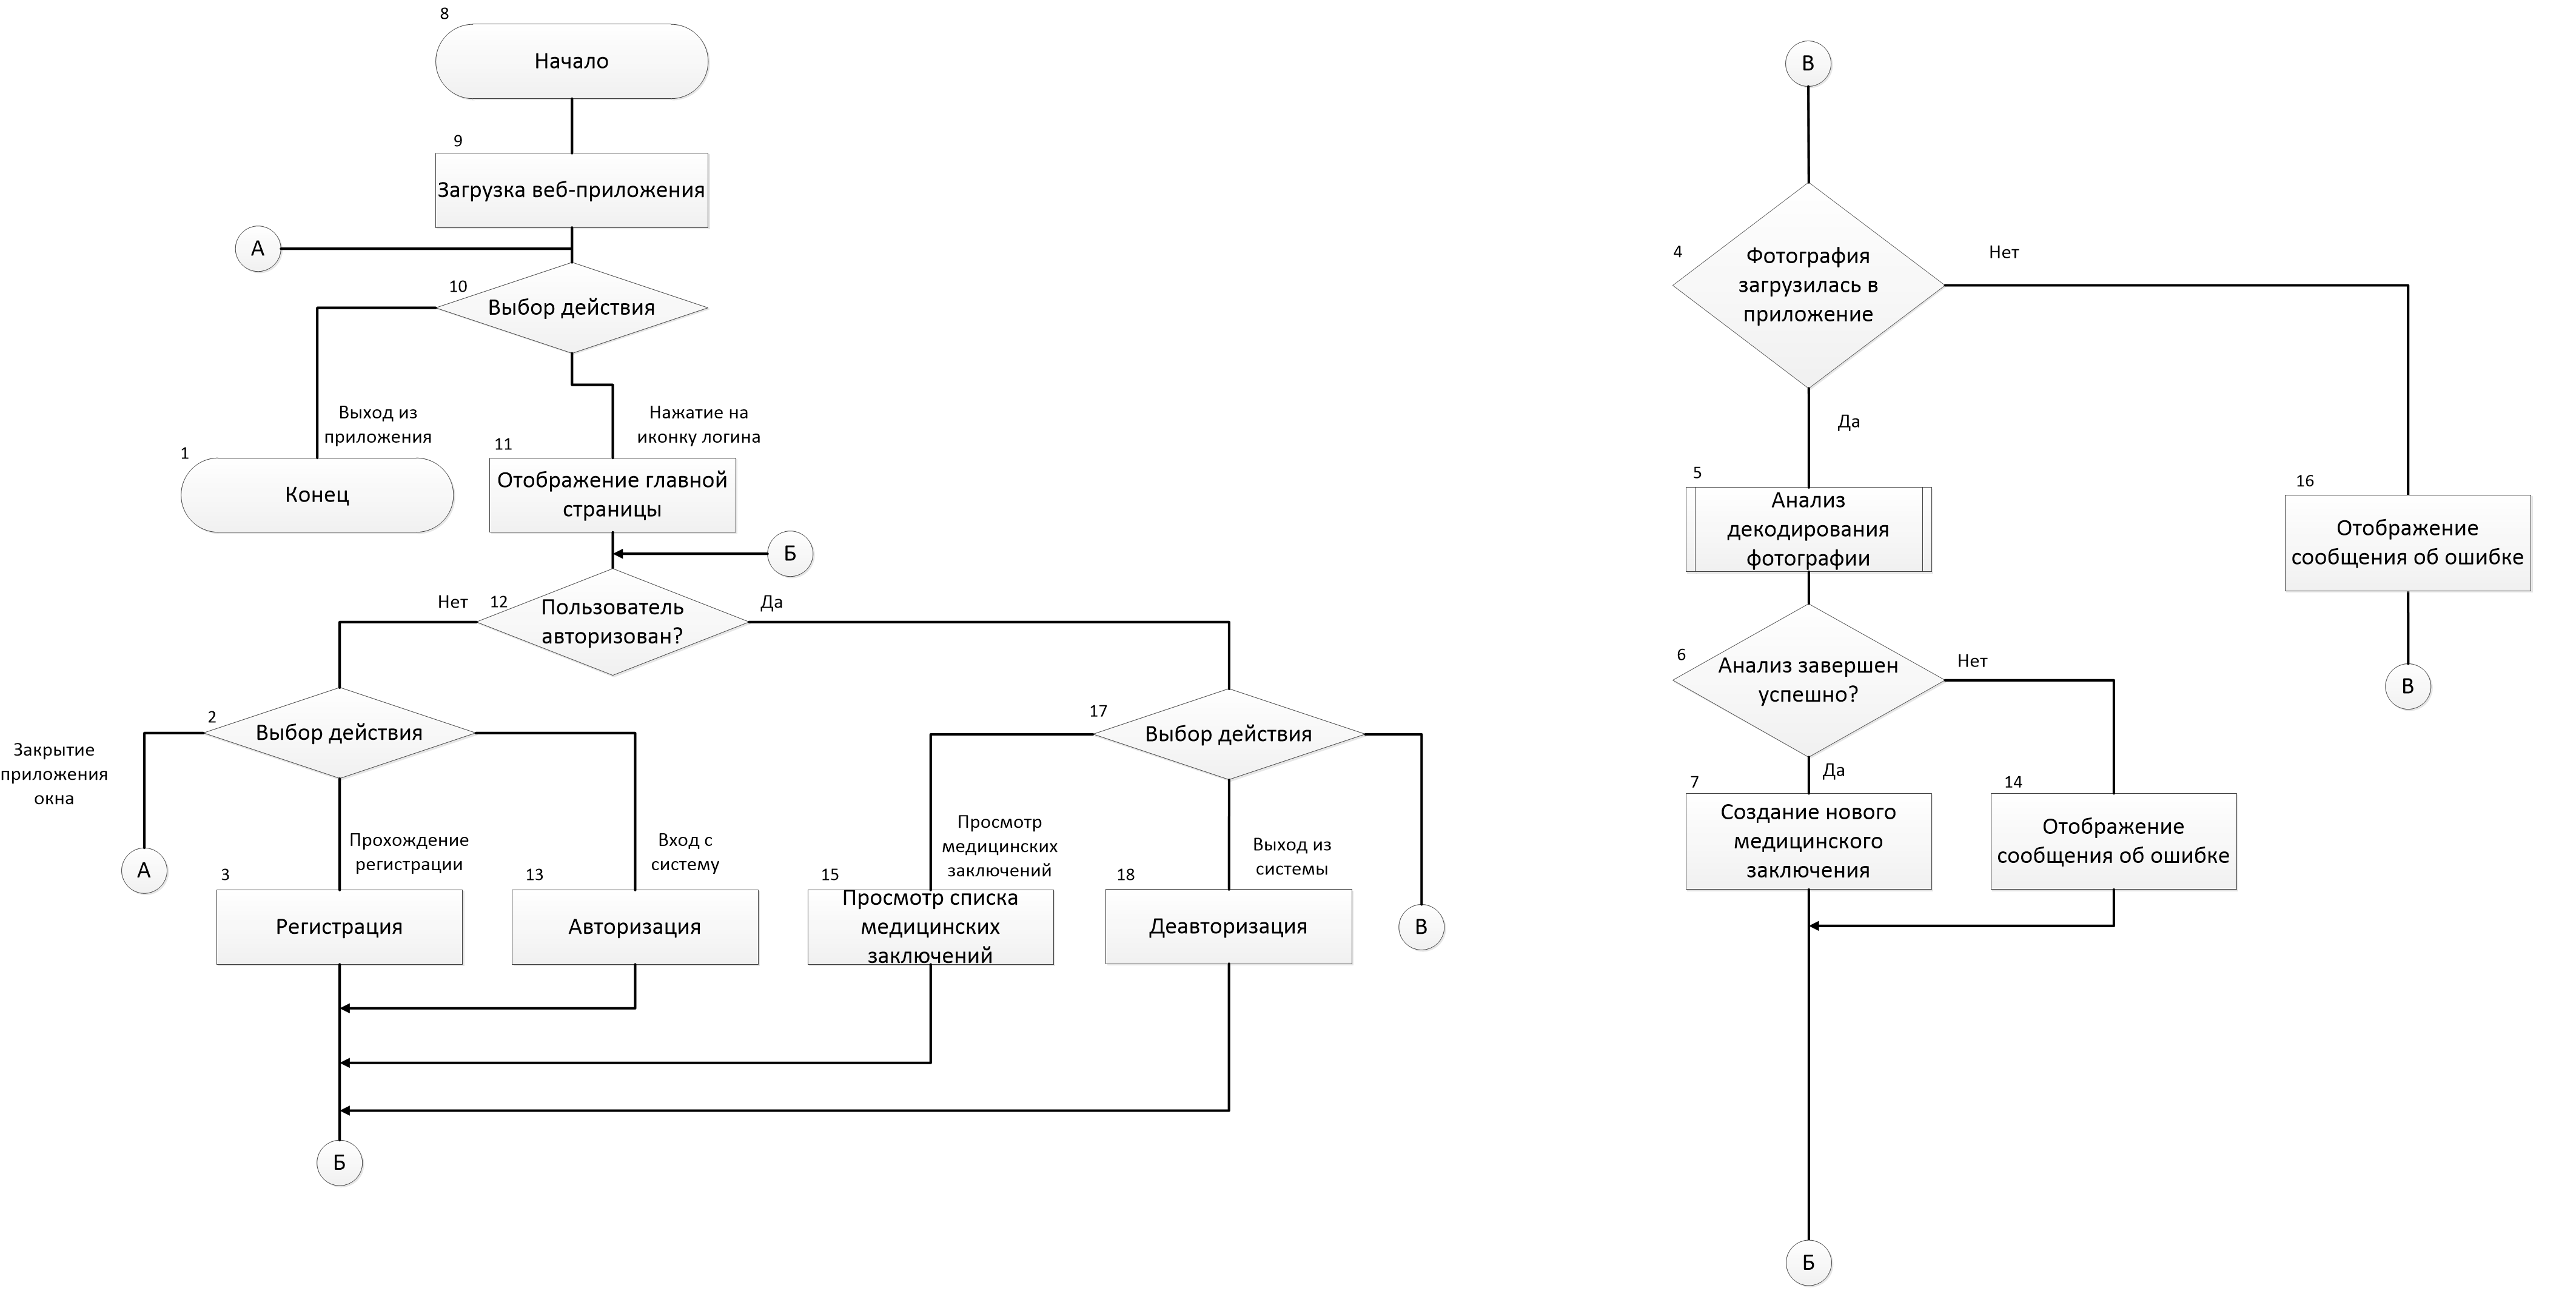
\includegraphics[scale=0.15]{spAlho.png}  
  \caption{Схема работы программы}
  \label{fig:domain:manual_structure:alho_sp}
\end{figure}

На рисунке~\ref{fig:domain:manual_structure:alho_sp} представлена схема работы клиентского приложения, которая демонстрирует алгоритм работы программного средства в целом. Из схемы можно увидеть, что пользователь может взаимодействовать с двумя частями клиентского приложения:

\begin{figure}[ht]
\centering
  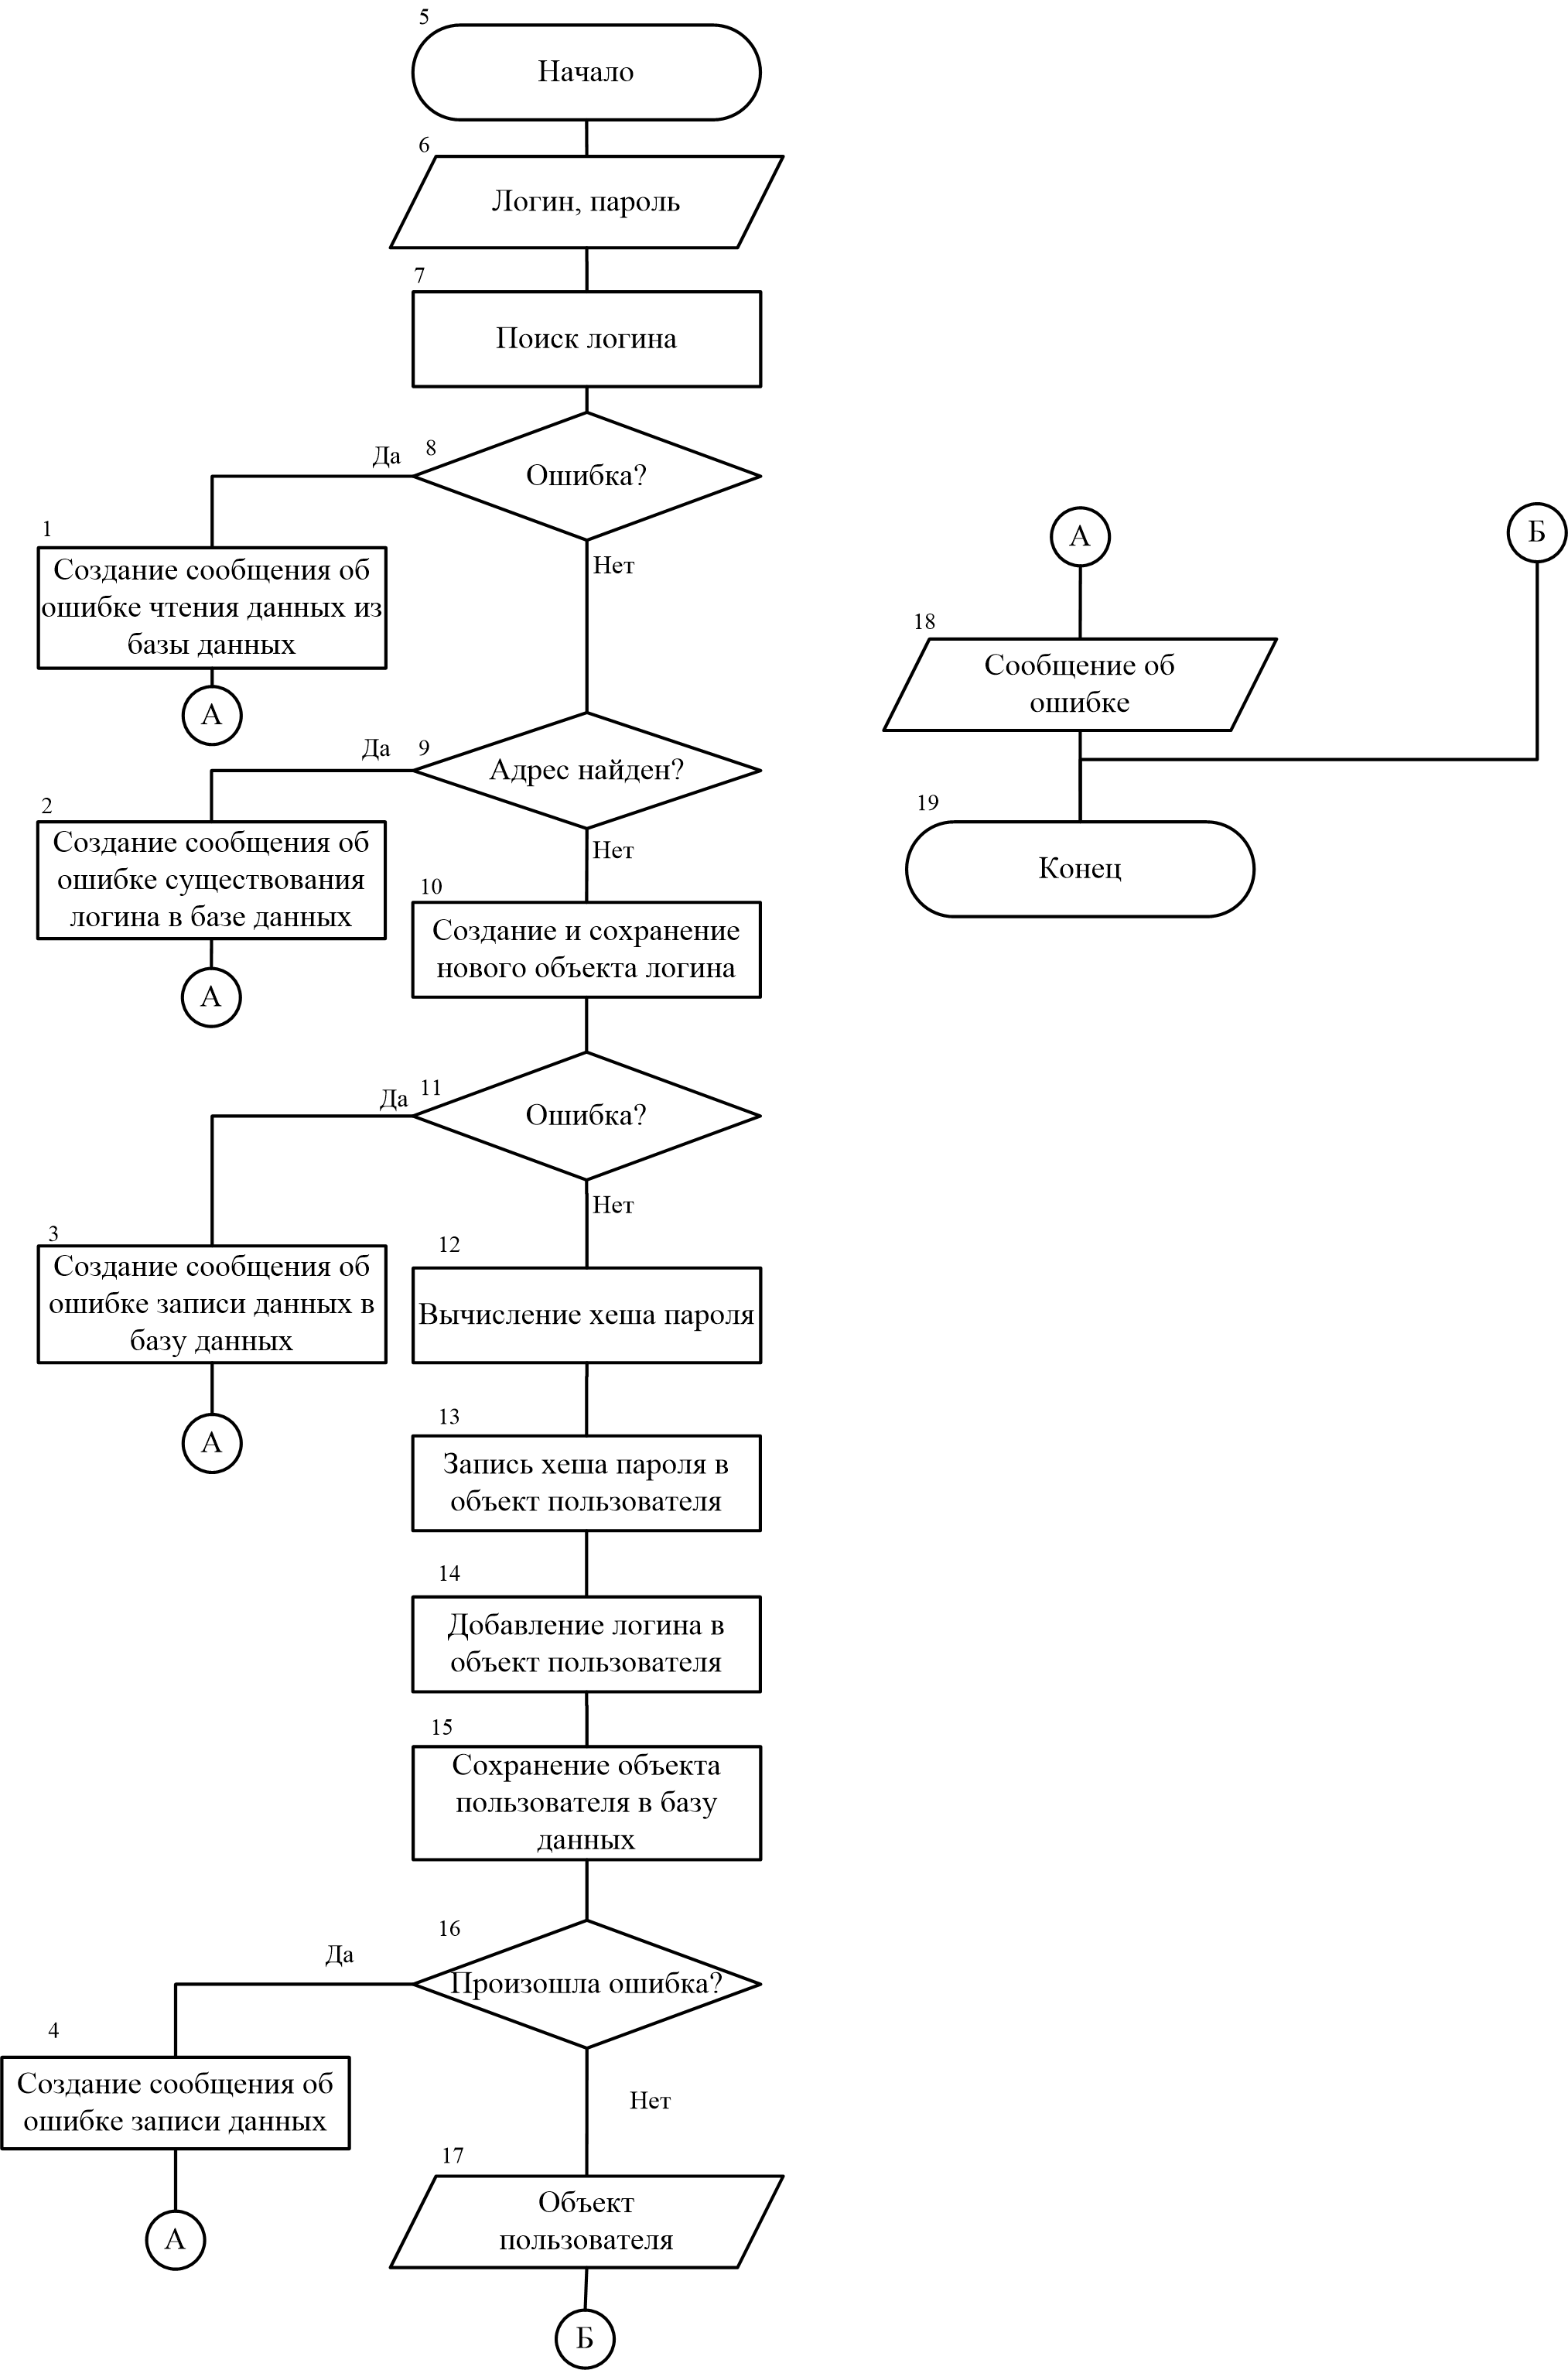
\includegraphics[scale=0.15]{systemRegistAlho.png}  
  \caption{Схема регистрации приложения}
  \label{fig:domain:manual_structure:alho_regist}
\end{figure}

\begin{figure}[ht]
\centering
  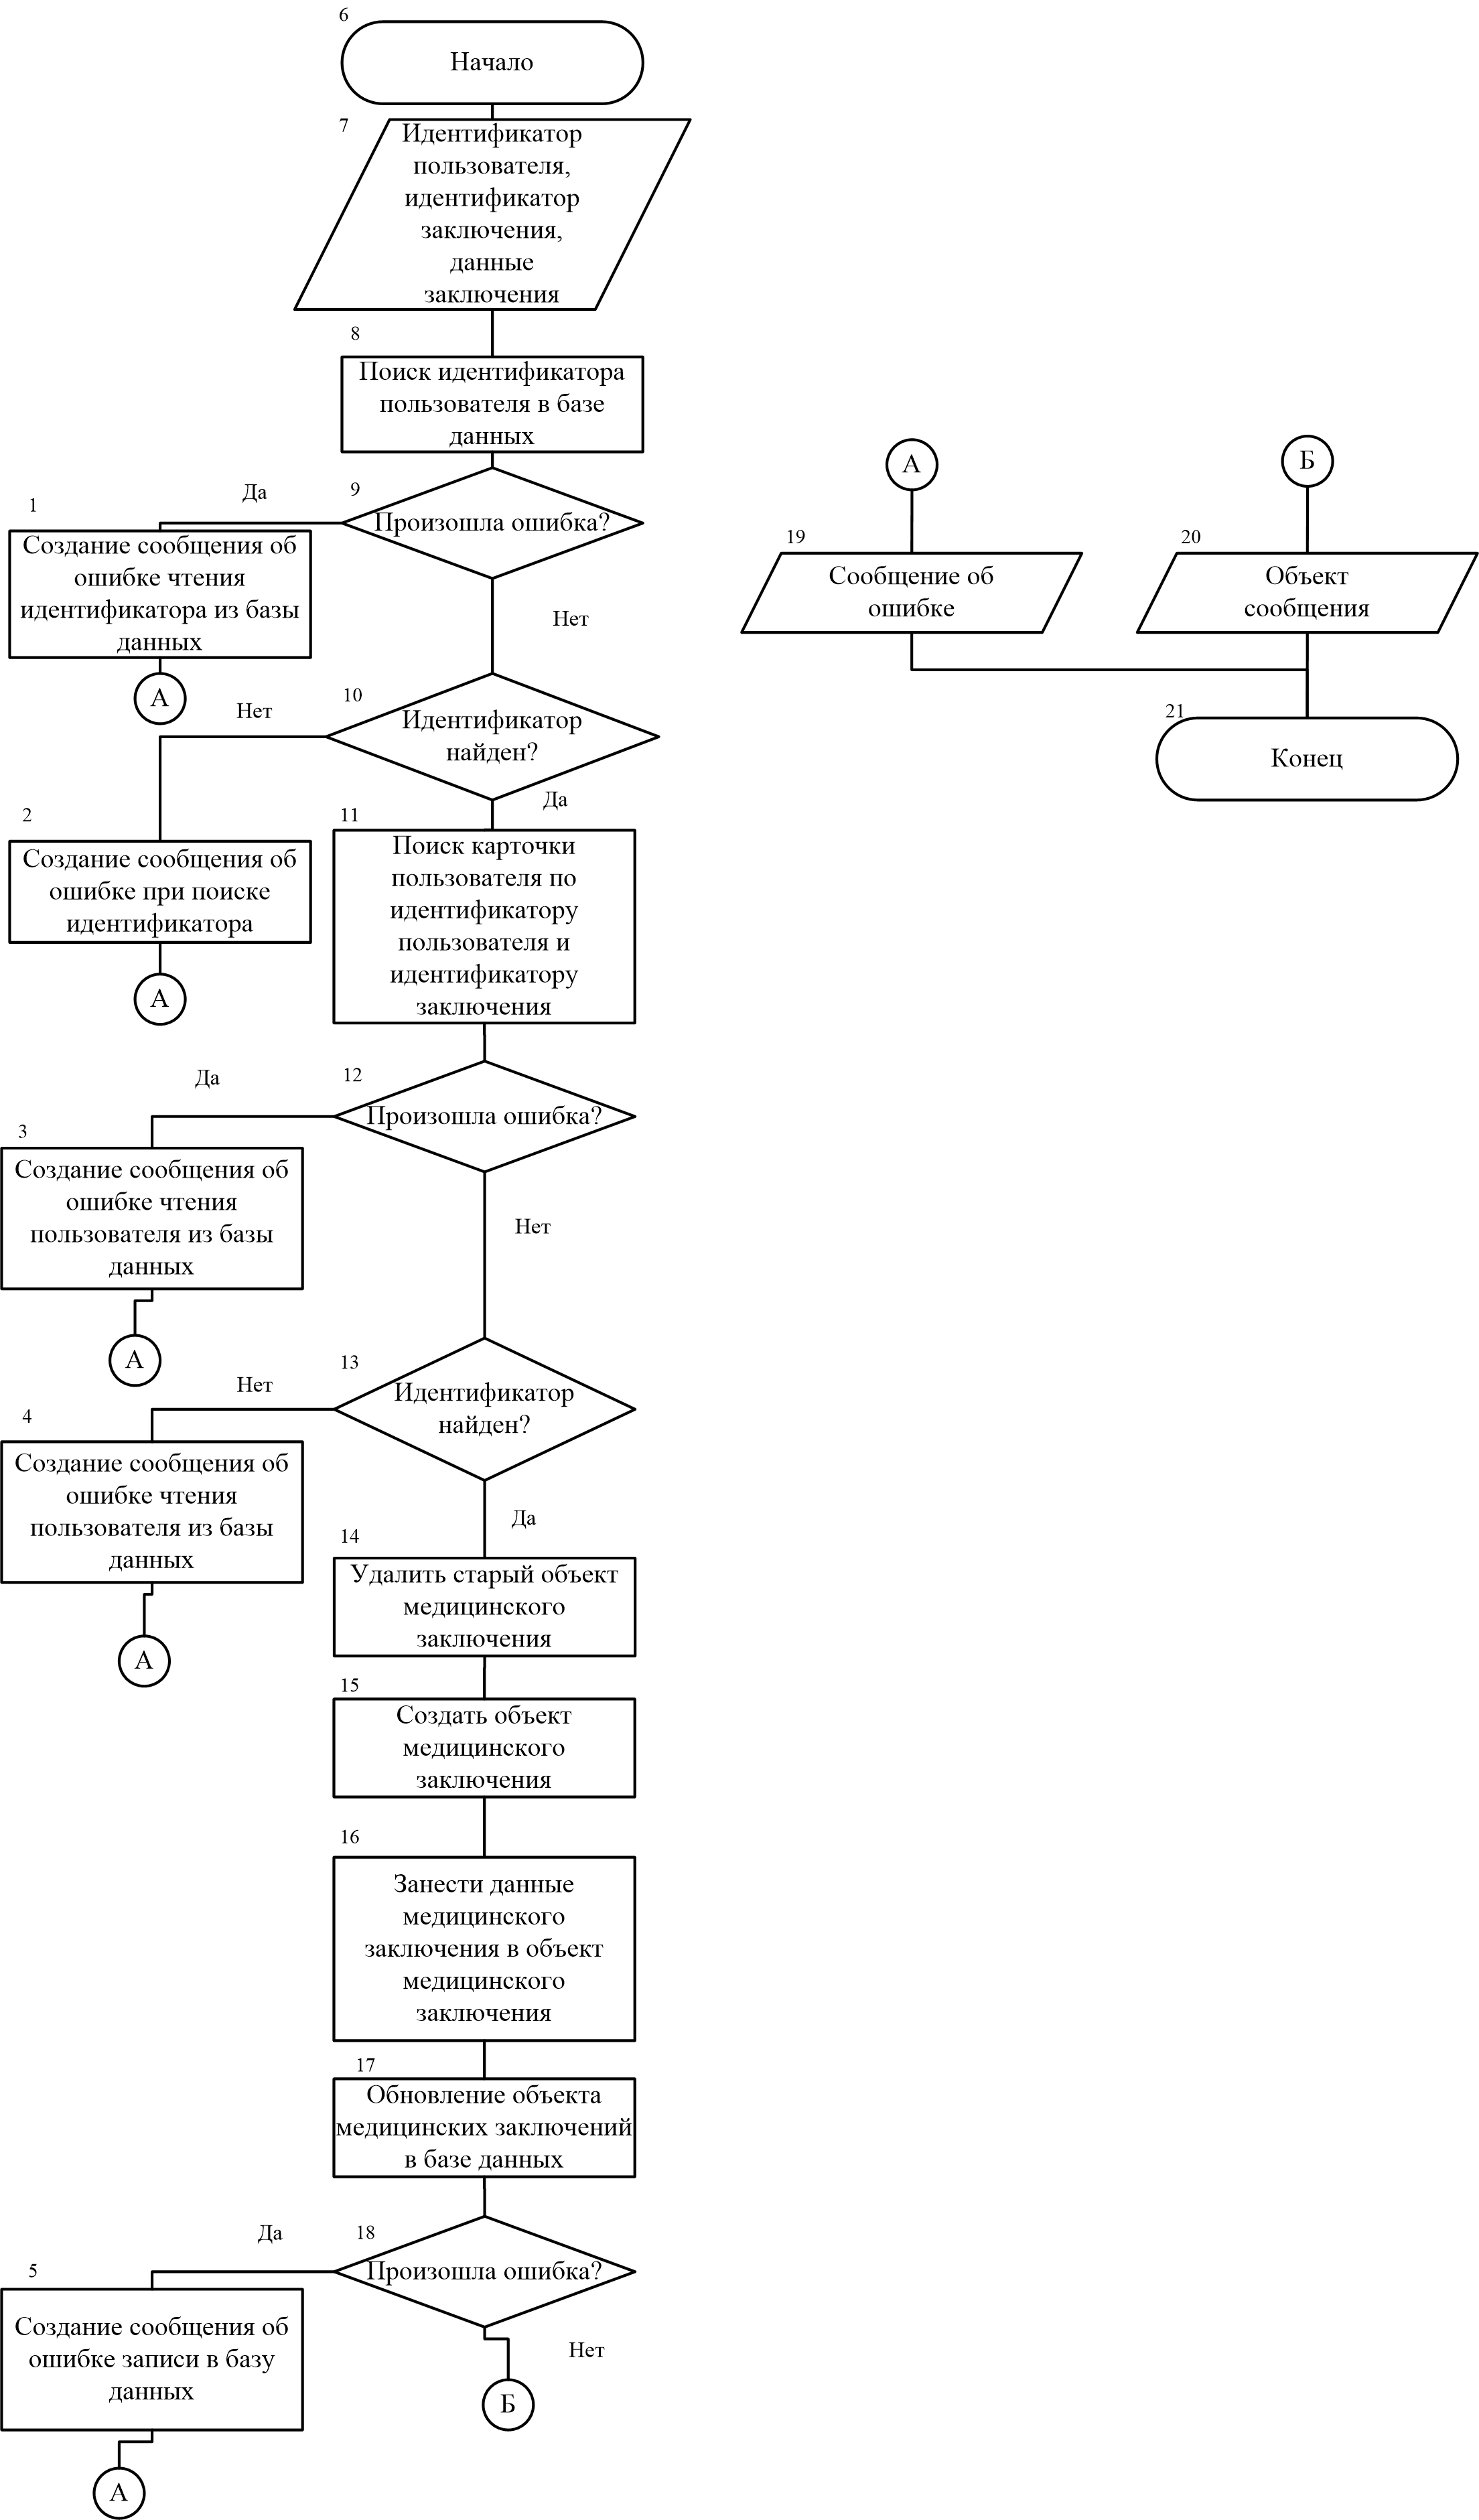
\includegraphics[scale=0.15]{systemEditMed.png}  
  \caption{Схема редактирования заключения пользователя}
  \label{fig:domain:manual_structure:alho_edit}
\end{figure}

\begin{enumerate}
  \item с модулем карточек, который позволяет взаимодействовать различными способами с карточками;
  \item с модулем работы с изображением.
\end{enumerate}

На рисунке~\ref{fig:domain:manual_structure:alho_regist} представлена схема работы регистрации приложения. Пользователь должен ввести валидные емэйл и пароль, чтобы пройти регистрацию. Суть алгоритма заключается в проверке введенной пользователем информации и сохранением полученого объекта пользователь в базу данных. 

Проверок поставленно несколько. Одна из них, на возможность записи в базу данных. После чего производится поиск введенного емэйла, и если он уже совпадает с существующим, то выдастся ошибка. Для лучшей защищенности, пароль не хранится в открытом доступе в базе данных, а сначала делается комбинирование пароля с <<солью>>, после чего производится хэширование по методу MD5. Для аутентификации, производятся ровно теже самые манипуляции с паролем, после чего сравнивается с результатом хэширования и значения, которое лежит в базе данных. 

На рисунке~\ref{fig:domain:manual_structure:alho_edit} представлена схема работы редактирование медицинских заключений. В самом начале алгоритма производится поиск существующего заключения в базе данных и если такое медицинское заключение найдено, то оно заменяется вновь созданным заключением.

Веб-сервер приложения будет представлять собой приложение, построенное на концепции модифицированной архитектуры MVC со слоями. На текущий момент, это одна из востребованных архитектур, позволяющая разделить на модули приложение. Принцип модульности является средством упрощения задачи проектирования ПС и распределения процесса разработки ПС между группами разработчиков. При разбиении ПС на модули для каждого модуля указывается реализуемая им функциональность, а также связи с другими модулями. Удобство использования модульной архитектуры заключается в возможности обновления (замены) модуля, без необходимости изменения остальной системы. Разделение на слои производится следующим образом:
\begin{enumerate}
  \item слой отражения модели на таблицу в базе данных(ML);
  \item слой доступа к данным (DAL);
  \item слой бизнес логики (BLL);
  \item слой управления (Controller).
\end{enumerate}

\begin{figure}[ht]
\centering
  \includegraphics[scale=0.3]{structurServer.png}  
  \caption{Структура серверного-приложения при использовании модифицированной архитектуры MVC}
  \label{fig:domain:manual_structure:structural_server}
\end{figure}

Слой управления представляет собой управленческий механизм, который обеспечивает связь между пользователем сервера и непосредственно самого сервера. Его основная задача отвечать на запросы пользователя и выдавать ему корректные результаты. Также одной из дополнительных функций является контроль переданных данных от пользователя.

Слой доступа к данным предоставляет интерфейс для определенного рода операций взаимодействия внешних слоев с источником данных, в данном случае с объектами моделей.

Слой бизнес-логики описывает основные функции приложения, предназначенные для достижения поставленных перед ним целей.

Слой отражения модели на таблицу в базе данных представляет собой совокупность объектов, связанных между собой и дополненных в последующем определенного вида параметрами для легкой доступности самих моделей.

На рисунке~\ref{fig:domain:manual_structure:structural_server} представлена структура серверного приложения на основе модифицированной MVC архитектуры. Такая структура имеет следующие преимущества:
\begin{itemize}
  \item подход позволяет производить параллельную разработку;
  \item возможность заменять слои, не нарушая тем самым целостность приложения;
  \item возможность протестировать каждый из слоев независимо друг от друга.
\end{itemize}

Клиентское приложение будет представлять собой приложение, построенное на концепции архитектуры Redux с основными принципами:
\begin{enumerate}
  \item состояние всего приложения сохранено в дереве объектов внутри одного хранилища (Store);
  \item единственный способ изменить состояние - это применить действие (Action).
\end{enumerate}

\begin{figure}[ht]
\centering
  \includegraphics[scale=0.5]{reduxFlow.png}  
  \caption{Структура клиентского-приложения при использовании архитектуры Redux}
  \label{fig:domain:manual_structure:structural_client}
\end{figure}

Действия -- это структура, которая передает данные из приложения в хранилище. Они являются единственными источниками информации для хранилища. Действия яаляются обычными JavaScript объектами.

Редьюсер -- чистая функция, которая принимает предыдущее состояние и действие и возвращает следующее состояние.

Хранилище -- объект, который соеденяет все части вместе. Хранилище берет на себя следующие задачи:
\begin{itemize}
  \item содержать состояние приложения (state);
  \item предоставлять доступ к состоянию приложения;
  \item предоставлять возможность обновления состояния.
\end{itemize}

На рисунке~\ref{fig:domain:manual_structure:structural_client} представлена структура клиентского-приложения она имеет следующие преимущества:
\begin{itemize}
  \item позволяет использовать компонентный подход в разработке;
  \item делает изменение состояние предсказуемым;
  \item позволяет использовать функциональный подход.
\end{itemize}

\subsection{Разработка алгоритма крипто-сервиса }
\label{sub:arch_and_mod:alholib-crypto}

В дипломном проекте необходимо передавать данные от серверной части к клиентской. Чтобы не произошел перехват данных и их изменения необходимо разработать крипто-сервис, который обеспечит сохранность и достоверность информации, передаваемой от сервера к клиенту.

Для этого был разработан алгоритм AES-128 -- симметричный алгоритм блочного шифрования. Этот алгоритм преобразует один 128-битный блок в другой, используя секретный ключ который нужен для такого преобразования. Для расшифровки полученного 128-битного блока используют второе преобразование с тем же секретным ключом.

Размер блока всегда равен 128 бит. Размер ключа также имеет фиксированный размер. Чтобы зашифровать произвольный текст любым паролем можно поступить так: 

\begin{itemize}
  \item получить хеш от пароля;
  \item преобразовать хеш в ключ по правилам описанным в стандарте AES;
  \item разбить текст на блоки по 128 бит;
  \item зашифровать каждый блок функцией cipher.
\end{itemize}

\begin{figure}[ht]
\centering
  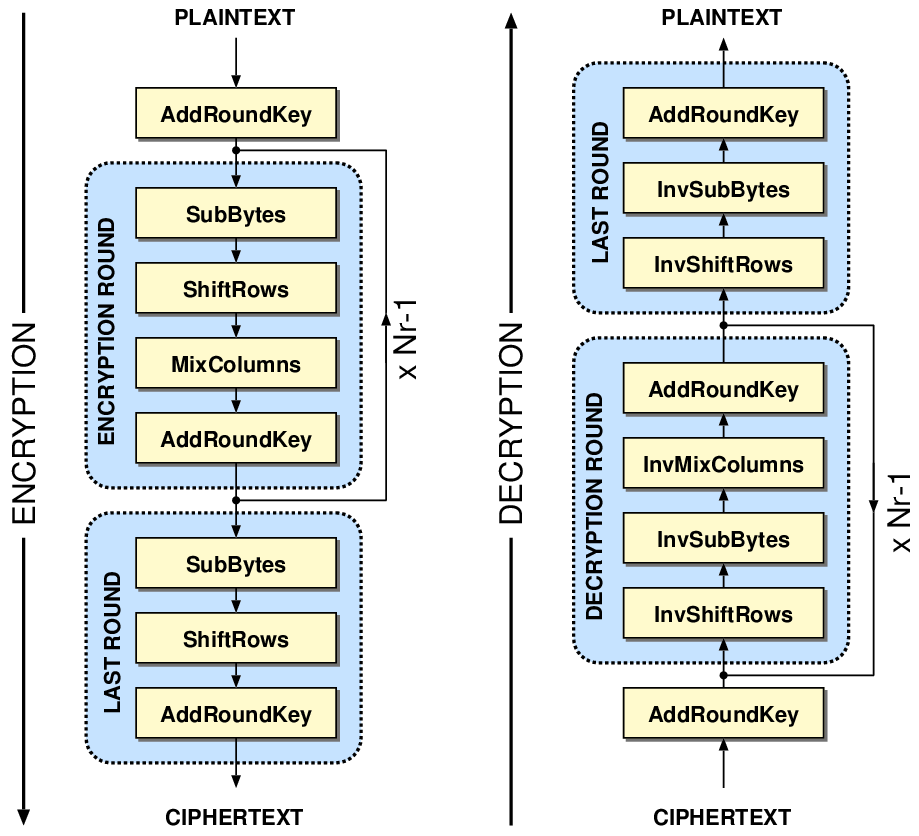
\includegraphics[scale=0.3]{alho_aes.png}  
  \caption{Структура алгоритма AES}
  \label{fig:domain:manual_structure:structural_aes}
\end{figure}

На рисунке~\ref{fig:domain:manual_structure:structural_aes} представлен алгоритм шифрования на вход которого приходит 128-битный блок данных plaintext и расписание ключей w, которое получается после KeyExpansion. 16-байтый plaintext он записывает в виде матрицы s размера 4Nb, которая называется состоянием AES, и затем Nr раз применяет к этой матрице 4 преобразования. В конце он записывает матрицу в виде массива и подаёт его на выход -- это зашифрованный блок. Каждое из четырёх преобразований очень простое.

AddRoundKey берёт из расписания ключей одну матрицу размера 4Nb и поэлементно добавляет её к матрице состояния. Если два раза применить AddRoundKey, то ничего не изменится, поэтому преобразование обратное к AddRoundKey это оно само.

SubBytes заменяет каждый элемент матрицы состояния соответвующим элементом таблицы SBox. Преобразование SubBytes обратимо. Обратное к нему находится с помощью таблицы InvSBox.

ShiftRows сдвигает i-ую строку матрицы s на i позиций влево, считая i с нуля. Обратное преобразование InvShiftRows сдвигает строки вправо.

MixColumns умножает каждый столбец матрицы s слева на особую матрицу размера 4 на 4.



\section{Создание программного средства} % (fold)
\label{sec:arch_and_mod}

\subsection{Описание классов, атрибутов и методов}
\label{sub:arch_and_mod:graphlib}

Перед началом создания мобильного программного средства необходимо определить список используемых языков программирования, библиотек и технологий, которые будут использоваться для написания приложения.

Для разработки мобильного программного средства, реализуемого в ходе данного дипломного проекта, выбран язык программирования JavaScript. Причина выбора обусловлена некоторыми факторами.

JavaScript является на текущий момент самым высокоразвивающимся и популярным языком программирования. Он имеет очень большое сообщество разработчиков, которые постоянно создают новые библиотеки и дополняют тем самым сам язык и его возможности.

JavaScript является однопоточным языком программирования и это тоже является плюсом. Во-первых, если необходимо распораллеливания определенных функций можно применять асинхронность, которая очень хорошо развита в данном языке программирования, во-вторых, нет необходимости создавать отдельный поток или брать из пула-потоков каждый раз, когда необходимо сделать определенного рода запрос.

JavaScript является мультипарадигменным языком, что позволяет реализовать функции различными способами. Есть возможность использовать объектно-ориентированную парадигму, так и функциональный подход. JavaScript не является функциональным языком программирования, однако, он содержит огромное количество свойств пресущих функциональным языкам:

\begin{itemize}
  \item функции являются объектами высшего порядка;
  \item функции являются объектами высшего порядка;
  \item работа с асинхроностью;
  \item частичное применение функций (carring);
  \item композиция функций (carring).
\end{itemize}

В ходе дипломного проета используется именно фунциональный подход, так как он является более производительным и легко тестируемым. Однако кроме нативного языка используются и дополнительные платформы, библиотеки и фреймворки.

Чтобы JavaScript можно было использовать для разработки мобильного приложения используется платформа Cordova. Cordova позволяет без знания нативной разработки под мобильные телефоны, использовать: JavaScript, HTML, CSS, которые впоследующем компилирует и переводит в машинные команды для определенных видов мобильных операционных систем. 

Суть самой платформы -- встраивание браузера WebView в мобильное приложение. По умолчанию Cordova представляет базовые функции браузера, однако функциональность можно расширить, путем добавления плагинов. Каждый плагин содержит в себе унифицированный интерфейс, позволяющий работать с определенной функциональностью. 

В дипломном проекте используются два плагина:
\begin{itemize}
  \item Плагин для работы с камерой телефона;
  \item Плагин добавляющий в браузер спиннер-загрузки.
\end{itemize}

Для разработки клиентской части приложения  будут использованы следующие библиотеки:
\begin{enumerate}
\item ReactJS;
\item ImmutableJS;
\item Tesseract;
\item Mocha.
\end{enumerate}

ReactJS -- библеотека построеная на концепции компонентов. В основе ReactJS лежит парадигма реактивного программирования. Данная парадигма позволяет описывать данные в виде набора некоторых утверждений или формул. Также создатели React полностью переработали идеалогию работы с DOM элементами. Была реализована новая работа с DOM назыающаяся теневой DOM. Фреймворк использует ее, чтобы при изменении состояния компонента судить о том, что поменять необходимо в реальном DOM и как это сделать наиболее эффективно.

ImmutableJS -- библиотека позволяющая сделать неизменняемые объекты, листы или массивы. Неизменяемость -- основной принцип функционального программирования.

Tesseract -- библиотека для считывания информации с изображений.

Mocha -- эта библиотека содержит общие функции для тестирования, включая describe и it. Позволяет протестировать клиентскую часть приложения дипломного проекта.

Рассмотрим основные классы и методы клиентской части мобильного-приложения представленного на изображении~\ref{fig:domain:manual_structure:client_class}.

\begin{figure}[ht]
\centering
  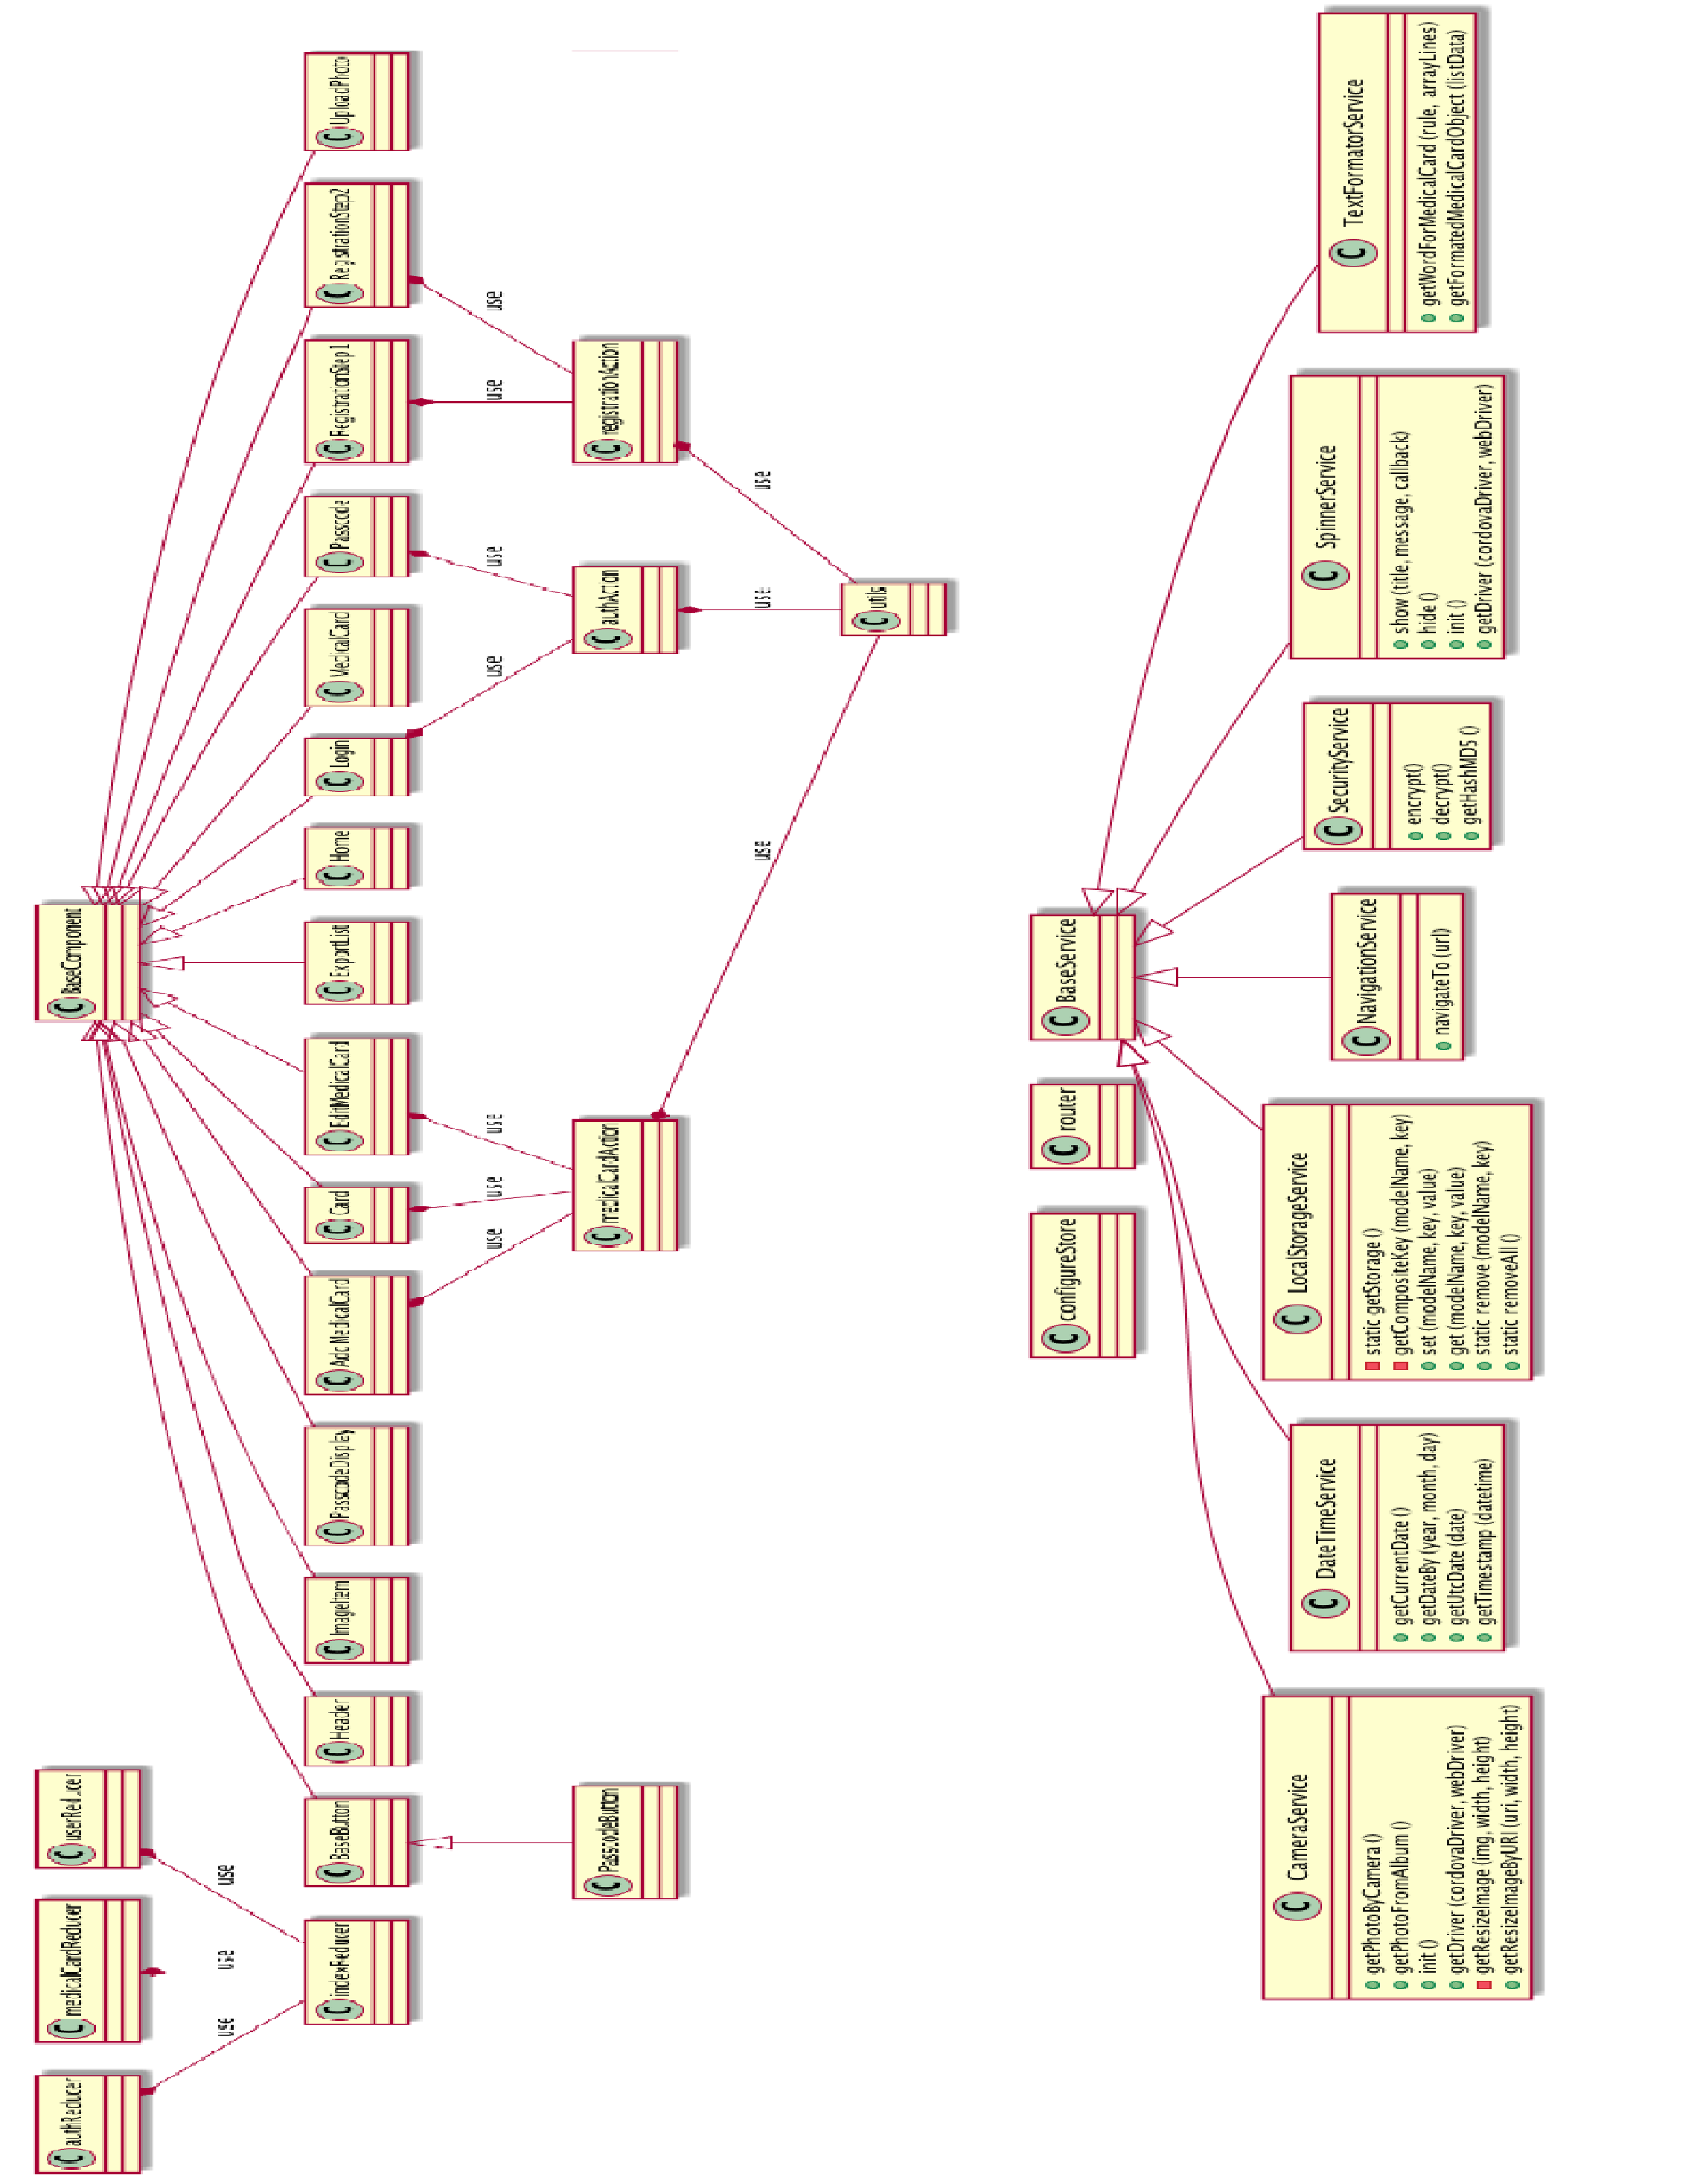
\includegraphics[scale=0.36]{ClassDiagram1.png}  
  \caption{Диаграмма классов компонентов и сервисов}
  \label{fig:domain:manual_structure:client_class}
\end{figure}

Класс ConfigureStore создает и конфигурирует единственное хранилище клиентского-приложения. Содержит единственный метод createStore, который создает хранилище с возможностью отслеживать постоянно его состояние на текущий момент, используется для логинга в приложении.

Класс CordovaCameraDriver создает интерфейс для работы с плагиной CordovaCamera. Содержит одноименные функции плагина: getPicture, distinationType, pictureSourceType. Также содержит в себе метод init, которым производится инициализация данного плагина и его полная конфигурация.

Класс WebCameraDriver создает интерфейс, но уже не для работы с плагином CordovaCamera, а интерфейс для работы с веб-клиентом, так как данное приложение можно будет открыть и на desctop версии, так как оно является кроссплатформенным.

Класс CameraService предоставляет возможность различного рода обработки полученной фотографии от интерфейса CordovaCameraDriver. Основные методы:
\begin{itemize}
  \item getPhotoByCamera достает информацию и саму фотографию, используя интерфейс CordovaCameraDriver;
  \item getResizeImage позволяет изменить размер самой фотографии, до формата, который будет пригоден в дальнейшем использовании;
  \item drawOnCanvas позволяет отрисовать изображение на canvas элементе, для последующей его обработки.
\end{itemize}

Класс LocalStorageService предоставляет возможность работы с браузерным localStorage. Основные методы:
\begin{itemize}
  \item getLocalStorage достает всю информацию из LocalStorage;
  \item getItem позволяет определенный элемент из LocalStorage;
  \item setItem позволяет добавить элемент в LocalStorage;
  \item clear позволяет очистить LocalStorage.
\end{itemize}

Класс SecurityService предоставляет возможность шифрования информации. Использует алгоритм шифрования AES-128 и MD5. Основные методы:
\begin{itemize}
  \item getMD5 достает хэш-функцию, используя алгоритм хэширования MD5;
  \item encrypt шифрует информацию используя алгоритм AES-128;
  \item decrypt дешифрует информацию;
  \item cipher -- тело самого алгоритма шифрования AES-128.
\end{itemize}

Класс TextFormatorService предоставляет возможность создания PDF-документа из JavaScript объекта. Производит парсинг самого объекта используя метод getFormatedMedicalCardObject, который в свою очередь распаршивает информацию полученную с фотографии, представленную в строковом формате. После чего, используя getPDFDocument полученный распаршенный объект сетится в PDF документ.

Классы AuthReducer, MedicalCardReducer, UserReducer представляют собой редьюсеры (чистые функции) для работы с авторизацией или регистрацией, медицинскими карточками, юзером соответственно. В них производится изменение текущего состояния определенного state на новое.

Классы Auth, MedicalCard, Medication, Registration представляют собой Action-объекты, которые содержат в себе обязательное поле типа экшена и второстепенные поля, необходимы для редьюсеров.

Также стоит обратить внимание на определенные функции в компонентах:
\begin{itemize}
  \item takeImport получает изображение, модифицирует его используя фильтры и передает Tesseract библиотеке, которая в свою очередь возвращает распознанный текст с изображения;
  \item handleExport переводит, получаемый объект, в PDF-документ;
  \item setData устанавливает полученные данные с пользовательского ввода в медицинскую карточку, формируя тем самым объект.
\end{itemize}

Каждый компонент содержит несколько обязательных методов. Одним из них является метод render. Он необходим для построения DOM дерева данного представления на основе его шаблона. После построения DOM дерева его корень записывается в атрибут элемента представления.

Метод GetDefaultProps вызывается единожды для класса компонента. Возвращаемый объект используется для свойст по умолчанию, если они не определены родительским компонентом.

Метод GetInitialState вызывается единожды для каждой инстанции компонента, давая возможность инициализировать кастомное состояние каждой инстранции.

Метод componentWillMount вызывается сразу же после начального рендеринга. Это последний момент воздействия на состояние компонента, перед вызовом метода Render.

Метод componentDidMount вызывается при условии, что рендеринг страницы произошел успешно и настоящий DOM срендерен. Тем самым можно произвести некоторое изменения уже на срендеренном элементе.

Рассмотрим основные классы серверной части мобильного-приложения. Класс UserController является базовым контроллером для работы с информацией о пользователе системы. Он содержит все основные методы для работы с пользователем.

Метод register позволяет зарегестрироваться пользователю в системе. В самом методе используется метод валидации, который позволяет отследить введенную пользователем информацию, и, если она содержит не желательную информацию, то метод вернет соответствующую ошибку на клиент и определенный HTTP статус.

Метод login позволяет пользователю авторизоваться в системе, сообщив исходные данные: логин и пароль от своего аккаунта.

Метод addProfile позволяет пользователю добавить более подробную информацию о себе, тут также срабатывает валидация и если пользователь вводит не корректную информацию, сервер вернет ошибку и HTTP статус, сообщая клиентской части, что необходимо предупредить пользователя о неверной информации.

Метод checkPasscode позволяет проверить passcode, который пользователь введет, когда его приложение удалится из памяти. Сделано это для того, чтобы пользователь постоянно не проходил авторизацию, ведь в мобильном телефоне уже осталась информация о том, что он прошел аутентификацию.

Класс medicalCardController -- контроллер для работы с медицинской информацией пользователя. Содержит все основные методы для работы с медицинскими карточками.

\begin{itemize}
  \item addNewCard позволяет добавить новую карточку;
  \item editMedCard позволяет отредактировать выбранную карточку;
  \item setData позволяет удалить выбранную карточку;
  \item addMedication позволяет добавить в медицинскую карточку медикаменты, необходимые для принятия;
  \item addDiagnostic позволяет добавить информацию о диагностике;
  \item getAllMedCard позволяет достать все карточки пациента.
\end{itemize}

Класс cryptoHelper на стороне сервера производит шифрование или дешифрования используя алгоритм AES-256-cbc. Сделано это для того, чтобы была лучшая криптостойкость и чтобы если произойдет взлом криптошифра на стороне клиента, информация на стороне сервера осталась в сохранности, потому что используется уже другой алгоритм. Содержит в себе методы:
\begin{itemize}
  \item encrypt позволяет зашифровать информацию;
  \item decrypt позволяет дешифровать информацию;
  \item createHash позволяет создать новый хэш.
\end{itemize}

Класс validationHelper -- хэлпер для работы с валидацией введенной информацией от пользователя. Содержит в себе методы определения необходимых данных, а также их валидирования, чтобы пользователь не ввел не желательную информацию в систему.

Класс userService производит работу с пользователем на более низком уровне (DAL), производит работу уже непосредственно с объектами-моделями, которые в последующем установятся в базу данных, содержит методы:
\begin{itemize}
  \item registation создает модель нового пользователя и добавляет в базу данных;
  \item login находит пользователя и проверяет введенную им информацию с информацией в базе данных;
  \item checkPasscode находит пользователя и проверяет его пасскод;
  \item addProfile добавляет пользователю дополнительную информацию.
\end{itemize}

Класс medicalService производит работу с медицинскми карточками на уровне DAL, содержит в себе методы:
\begin{itemize}
  \item addMedicalCard создает модель медицинской карточки и заносит ее в базу данных;
  \item editMedicalCard находит определенную медицинскую карточку и изменяет ее в последующем заносит в базу данных;
  \item deleteMedicalCard находит медицинскую карточку и удаляет ее из базы данных;
  \item addDoctorForMedicalCard добавляет к медицинской карточке информацию о враче;
  \item addMedication добавляет к медицинской карточке информацию о медикаментах;
  \item addPaymentInfo добавляет к медицинской карточке информацию о оплате услуг;
  \item getAllMedicalCard достает все возможные медицинские карточки из базы данных.
\end{itemize}

\subsection{Инструкция по сборке ПС}
\label{sub:arch_and_mod:sbor}

\subsubsection{Инструкция и информация по сборке сервера}

Для обеспечения работы сервера необходимо выполнить следующую последовательность действий:
\begin{enumerate}
\item установить сервер NodeJS;
\item установить базу данных MongoDB;
\item выполнить команду npm install, которая установит дополнительные пакеты;
\item проинициализировать базу данных с помощь скрипта mongod;
\item запустить сервер используя команду node server.js.
\end{enumerate}

Для дипломного проекта используется облачный сервис Amazon, который предоставляет масштабируемые вычислительные ресурсы в облаке. На сервере Amazon необходимо произвести конфигурацию, чтобы он имел статический IP-адрес выбранного сервиса. После чего произвести установка операционной системы Ubuntu, после которой можно будет собрать сервер используя команды выше.

\subsubsection{Инструкция по сборке клиентского приложения}

Для обеспечения работы клиентского приложения необходимо выполнить следующую последовательность действий:
\begin{enumerate}
\item установить Java SDK;
\item установить Android Studio;
\item установить XCode;
\item скачать репозиторию Cordova;
\item установить плагины CordovaCamera и SpinnerCordova;
\item выполнить команду npm install, которая установит дополнительные пакеты;
\item выполнить команду cordova run android или cordova run ios.
\end{enumerate}

\section{Тестирование программного средства}
\label{sec:testing}

Для тестирования программного средства используются модульные и интеграционные тесты. Модульные тесты позволяют проверять отдельные участки программного средства на правильность их выполнения при определенных входных параметрах. Это позволяет достаточно быстро проверить, не привело ли очередное изменение кода к появлению определенного рода ошибок в уже оттестированных местах приложения, а также облегчает обнаружения и устранения таких ошибок. Цель модульного тестирования -- изолировать отдельные участки приложения и доказать, что по отдельности эти части являются работоспособными. 

Интеграционные тесты позволяют проверить правильность взаимодействия различных модулей программного средства друг с другом. При интеграционном тестирование отдельные модули приложения объеденяются в специальные модули и тестируются в совокупности.

Тест-кейсы для проверки базовой функциональности программного средства представлены в таблицах \ref{sec:testing:configuration_register}, \ref{sec:testing:configuration_login}  и \ref{sec:testing:data_storing}.

\begin{longtable}[l]{| >{\raggedright}p{0.3\textwidth}
                     | >{\raggedright}p{0.3\textwidth}
                     | >{\raggedright\arraybackslash}p{0.3\textwidth}|}
  \caption{Тестирование регистрации}
  \label{sec:testing:configuration_register} \tabularnewline

  \hline
       Название тест-кейса и его описание & Ожидаемый результат & Фактический результат результат \\
   \hline
   Регистрация\\ 
   1) Ввести в поле <<Login>> значение не существующего пользователя; \\
   2) ввести в поле <<Passcode>> значение из 4 цифр без пробелов; \\  
   3) ввести в поле <<Confirm passcode>> схожее значение с полем <<Passcode>>; \\ 
   4) нажать на кнопку <<Register>>.

   &
   1) Закрывается страница авторизации; \\
   2) появляется страница заполнения профиля.

   & Тест пройден \\
   \hline
\end{longtable}

\begin{longtable}[l]{| >{\raggedright}p{0.3\textwidth}
                     | >{\raggedright}p{0.3\textwidth}
                     | >{\raggedright\arraybackslash}p{0.3\textwidth}|}
  \caption{Тестирование авторизации}
  \label{sec:testing:configuration_login} \tabularnewline

  \hline
       Название тест-кейса и его описание & Ожидаемый результат & Фактический результат результат \\
   \hline
   Авторизация\\ 
   1) Ввести в поле <<Login>> значение существующего пользователя; \\
   2) ввести в поле <<Passcode>> значение из 4 цифр без пробелов, являющееся паролем пользователя; \\  
   4) нажать на кнопку <<Login>>.

   &
   1) Закрывается страница авторизации; \\
   2) появляется главная страница приложения.

   & Тест пройден \\
   \hline
\end{longtable}



\begin{longtable}[l]{| >{\raggedright}p{0.3\textwidth}                     
                     | >{\raggedright}p{0.3\textwidth}
                     | >{\raggedright\arraybackslash}p{0.3\textwidth}|}
  \caption{Тестирование выхода из спящего режима}
  \label{sec:testing:data_storing} \tabularnewline

  \hline
      Название тест-кейса и его описание & Ожидаемый результат & Фактический результат результат \\
   \hline
   Хранение данных в памяти\\ 
   1) Свернуть приложение и перейти на главную страницу мобильного телефона; \\
   2) запустить цикл удаления из памяти приложений;\\
   3) не очищать кэш;\\
   4) запустить приложение;\\
   5) набрать корректный, для текущего пользователя пасскод.

   &
   1) Закрывается страница пасскода;\\
   2) появляется главная страница приложения.\\

   &
   Тест пройден \\
   \hline
\end{longtable}

Тестирование основной функциональности мобильного программного средства будет представлен в таблицах \ref{sec:testing:degradation_1}, \ref{sec:testing:degradation_2}  и \ref{sec:testing:degradation_3}.

\begin{longtable}[p]{| >{\raggedright}p{0.3\textwidth}                     
                     | >{\raggedright}p{0.3\textwidth}
                     | >{\raggedright\arraybackslash}p{0.3\textwidth}|}
  \caption{Тестирование процесса создания медицинского заключения}
  \label{sec:testing:degradation_1} \tabularnewline

  \hline
      Название тест-кейса и его описание & Ожидаемый результат & Фактический результат результат \\
   \hline
   Создание медицинского заключения\\ 
   1) На главной странице приложения открыть пункт <<Medical Card>>; \\
   2) нажать на кнопку <<+>>;\\
   3) заполнить все информационные поля в открывшейся странице;\\
   4) нажать на кнопку <<Save>>.

   &
   1) Закроется страница создания нового медицинского заключения;\\
   2) откроется главная страница приложения.

   &
   Тест пройден \\
   \hline
\end{longtable}

Создавать медицинские заключения можно и без использовании всех информативных полей. Главными полями медицинского заключения является: информация о докторе, дата создания медицинского заключения, общая информация о заключении.

Все остальные поля являются лишь дополнением, то есть информация об оплате и медикаментах, можно спокойно опустить и тест-кейс представленный в таблице \ref{sec:testing:degradation_1} все равно будет пройден.

Стоит также упомянуть, что создание медицинского заключения является основной информационной базой мобильного приложения. Для всех пользователей приложения будет создана отдельная информационная база, тем самым можно быть уверенным, что данные будут конфиденциально сохранены.

\pagebreak

\begin{longtable}[p]{| >{\raggedright}p{0.3\textwidth}                     
                     | >{\raggedright}p{0.3\textwidth}
                     | >{\raggedright\arraybackslash}p{0.3\textwidth}|}
  \caption{Тестирование процесса редактирования медицинского заключения}
  \label{sec:testing:degradation_2} \tabularnewline

  \hline
      Название тест-кейса и его описание & Ожидаемый результат & Фактический результат результат \\
   \hline
   Редактирование медицинского заключения\\ 
   1) На главной странице приложения открыть пункт <<Medical Card>>; \\
   2) из представленного списка выбрать медицинское заключение;\\
   3) в открывшемся окне информации о медицинском заключении нажать на кнопку <<E>>;\\
   4) заполнить все информационные поля в открывшейся странице;\\
   5) нажать на кнопку <<Save>>.

   &
   1) Закроется страница редактирования медицинского заключения;\\
   2) откроется главная страница приложения.

   &
   Тест пройден \\
   \hline
\end{longtable}

\pagebreak

\begin{longtable}[p]{| >{\raggedright}p{0.3\textwidth}                     
                     | >{\raggedright}p{0.3\textwidth}
                     | >{\raggedright\arraybackslash}p{0.3\textwidth}|}
  \caption{Тестирование процесса удаления медицинского заключения}
  \label{sec:testing:degradation_3} \tabularnewline

  \hline
      Название тест-кейса и его описание & Ожидаемый результат & Фактический результат результат \\
   \hline
   Удаление медицинского заключения\\ 
   1) На главной странице приложения открыть пункт <<Medical Card>>; \\
   2) из представленного списка выбрать медицинское заключение;\\
   3) в открывшемся окне информации о медицинском заключении нажать на кнопку <<D>>.

   &
   1) Закроется страница информации медицинского заключения;\\
   2) откроется главная страница приложения.

   &
   Тест пройден \\
   \hline
\end{longtable}

Следует протестировать поведение системы при наличии в памяти многократных ошибок. Для этого запускаются тесты из таблицы \ref{sec:testing:regeneration}.
\begin{longtable}[p]{| >{\raggedright}p{0.3\textwidth}                     
                     | >{\raggedright}p{0.3\textwidth}
                     | >{\raggedright\arraybackslash}p{0.3\textwidth}|}
  \caption{Тестирование процесса регенерации  памяти при сдвинутом периоде обновления}
  \label{sec:testing:regeneration} \tabularnewline

  \hline
      Название тест-кейса и его описание & Ожидаемый результат & Фактический результат результат \\
   \hline
   Регенерация памяти\\ 
   1) Инициализировать объект MemorySystem входными параметрами: путь к ini-файлу, путь к файлу конфигурации памяти, объем памяти, количество циклов, на которое сдвинут период обновления памяти; \\
   2) запустить цикл работы симулятора.

   &
   1) В консоли отображается информация о запуске системы и объеме симулируемой памяти;\\
   2) после наступления периода обновления появляется сообщение о несовпадении эталонной и тестовой сигнатур;\\
   3) появляется уведомление о запуске маршевого теста;\\
   4) маршевый тест пройден, неисправности не обнаружены.

   &
   Тест пройден \\
   \hline
\end{longtable}

В открытых источниках находится информация о покрывающей способности некоторых маршевых тестов, например MATS, MATS++ и других. На основе этой информации строятся тесты, для проверки правильности работы тестирующих алгоритмов ОЗУ. Тесты предполагают наличие файла неисправностей в формате csv. Общий алгоритм тестирования проверки работоспособности маршевых тестов един и сводится к таблице \ref{sec:testing:march_testing}.
\pagebreak

\begin{longtable}[p]{| >{\raggedright}p{0.3\textwidth}                     
                     | >{\raggedright}p{0.3\textwidth}
                     | >{\raggedright\arraybackslash}p{0.3\textwidth}|}
  \caption{Тестирование поведения системы при наличии в памяти неисправностей}
  \label{sec:testing:march_testing} \tabularnewline

  \hline
      Название тест-кейса и его описание & Ожидаемый результат & Фактический результат результат \\
   \hline
   Работоспособность маршевых тестов\\ 
   1) Инициализировать объект MemorySystem входными параметрами: путь к ini-файлу, путь к файлу конфигурации памяти, объем памяти, путь к файлу неисправностей; \\
   2) запустить цикл работы симулятора.

   &
   1) В консоли отображается информация о запуске системы и объеме симулируемой памяти;\\
   2) после наступления периода обновления появляется сообщение о несовпадении эталонной и тестовой сигнатур;\\
   3) появляется уведомление о запуске маршевого теста;\\
   4) маршевый тест не пройден, обнаружены неисправности.

   &
   Тест пройден \\
   \hline
\end{longtable}


%   \begin{longtable}{| >{\raggedright}p{0.20\linewidth} 
%                   | >{\raggedright}p{0.28\linewidth} 
%                   | >{\raggedright}p{0.28\linewidth} 
%                   | >{\raggedright\arraybackslash}p{0.12\linewidth}|}
%    \caption{Тестовые сценарии} \label{tab:long} \\

%    \hline
%    Идентификатор тест-кейса & Описание тест-кейса & Ожидаемый результат & Тестовый сценарий пройден Да/Нет \\
%    \endfirsthead

% \multicolumn{3}{l}%
% {{\raggedright Продолжение таблицы \thetable{}}} \\
% \hline
%    Идентификатор тест-кейса & Описание тест-кейса & Ожидаемый результат & Тестовый сценарий пройден Да/Нет \\
% \endhead
%    \hline
%    Login-1 &
%    			\vspace{-6.5mm} 
%    			\begin{enumerate} 
%    				\item[1)] Ввести в поле <<Login>> и поле <<Passcode>> не корректные значения;
% 				\item[2)] нажать на кнопку <<Log In>>.
% 			\end{enumerate}
%    			 & Появится сообщение <<Invalid login>> & Да \\

%    \hline
%    Login-2 & 
%    			\vspace{-6.5mm}
%    			\begin{enumerate} 
%    				\item[1)] Ввести в поле корректное значение <<Login>>;
% 				\item[2)] ввести в поле <<Passcode>> значение из символов;
% 				\item[3)] нажать на кнопку <<Log In>>.
% 			\end{enumerate}
% 			& Появится сообщение <<Passcode length should be 4 number>> & Да \\

%    \hline
%    Login-3 & 
%    			\vspace{-6.5mm}
%    			\begin{enumerate} \item[1)] Ввести в поле корректное значение <<Login>>;
% 				\item[2)] ввести в поле <<Passcode>> значение из более чем 4 цифр;
% 				\item[3)] нажать на кнопку <<Log In>>.
% 			\end{enumerate}
%    			& Появится сообщение <<Passcode length should be 4 number>> & Да \\
%    	\hline
%    Login-4 & 
%    			\vspace{-6.5mm}
%    			\begin{enumerate} \item[1)] Ввести в поле корректное значение <<Login>>;
% 				\item[2)] ввести в поле <<Passcode>> корректное значение из 4 цифр;
% 				\item[3)] нажать на кнопку <<Log In>>.
% 			\end{enumerate}
%    			& 
%    			\vspace{-6.5mm}
%    			\begin{enumerate} \item[1)] Закрывается страница авторизации;
% 				\item[2)] появляется главная страница приложения.
% 			\end{enumerate}
% 			& Да \\
%    \hline
%    Login-5 & \vspace{-6.5mm} \begin{enumerate} \item[1)] Ввести в поле корректное значение <<Login>>;
% 				\item[2)] ввести в поле <<Passcode>> значение из 4 цифр не являющуюся паролем данного пользователя;
% 				\item[3)] нажать на кнопку <<Log In>>.
% 			\end{enumerate}
%    			& Появится сообщение <<Invalid Passcode>> & Да \\
%    	\hline
%    	Login-6 & \vspace{-6.5mm} \begin{enumerate} \item[1)] Ввести в поле несколько пробелов, а после корректное значение <<Login>>;
% 				\item[2)] ввести в поле <<Passcode>> корректное значение из 4 цифр;
% 				\item[3)] нажать на кнопку <<Log In>>.
% 			\end{enumerate}
%    			& \vspace{-6.5mm} \begin{enumerate} \item[1)] Закрывается страница авторизации;
% 				\item[2)] появляется главная страница приложения.
% 			\end{enumerate}
% 			& Да \\
%    	\hline
%    	Register-1 & \vspace{-6.5mm} \begin{enumerate} \item[1)] Ввести в поле значение <<Login>>;
% 				\item[2)] ввести в поле <<Passcode>> корректное значение из 4 цифр без пробелов;
% 				\item[3)] ввести в поле <<Confirm Passcode>> другое значение из 4 цифр без пробелов;
% 				\item[4)] нажать на кнопку <<Register>>.
% 			\end{enumerate}
%    			& Появляется сообщение <<Not corrected passcode>>;
% 			& Да \\
%    	\hline
%    	Register-2 & \vspace{-6.5mm} \begin{enumerate} \item[1)] Ввести в поле значение <<Login>>;
% 				\item[2)] ввести в поле <<Passcode>> корректное значение из 4 цифр без пробелов;
% 				\item[3)] ввести в поле <<Confirm Passcode>> схожее значение с полем <<Passcode>>
% 				\item[4)] нажать на кнопку <<Register>>.
% 			\end{enumerate}
%    			& \vspace{-6.5mm} \begin{enumerate} \item[1)] Закрывается страница авторизации;
% 				\item[2)] появляется страница заполнения профиля.
% 			\end{enumerate}
% 			& Да \\
%    	\hline
%    	Register-3 & \vspace{-6.5mm} \begin{enumerate} \item[1)] Ввести в поле значение <<Login>>;
% 				\item[2)] ввести в поле <<Passcode>> значение из более чем 4 цифр без пробелов;
% 				\item[3)] ввести в поле <<Confirm Passcode>> схожее значение с полем <<Passcode>>
% 				\item[4)] нажать на кнопку <<Register>>.
% 			\end{enumerate}
%    			& Появится сообщение <<Passcode length should be 4 number>> & Да \\
%    	\hline
%    	Register-4 & \vspace{-6.5mm} \begin{enumerate} \item[1)] Ввести в поле значение <<Login>> существующего пользователя;
% 				\item[2)] ввести в поле <<Passcode>> корректное значение из 4 цифр без пробелов;
% 				\item[3)] ввести в поле <<Confirm Passcode>> схожее значение с полем <<Passcode>>
% 				\item[4)] нажать на кнопку <<Register>>.
% 			\end{enumerate}
%    			& Появится сообщение <<User consist in system>> & Да \\
%    	\hline
%    	Register-5 & \vspace{-6.5mm} \begin{enumerate} \item[1)] Ввести в поле значение <<Login>>;
% 				\item[2)] ввести в поле <<Passcode>> строку с пробелами и следом 4 цифры;
% 				\item[3)] ввести в поле <<Confirm Passcode>> схожее значение с полем <<Passcode>>
% 				\item[4)] нажать на кнопку <<Register>>.
% 			\end{enumerate}
%    			& Появится сообщение <<Passcode can't contain space>> & Да \\
%    	\hline
%    	Register-6 & \vspace{-6.5mm} \begin{enumerate} \item[1)] Ввести в поле значение <<Login>>;
% 				\item[2)] ввести в поле <<Passcode>> корректное значение из 4 цифр без пробелов;
% 				\item[3)] ввести в поле <<Confirm Passcode>> схожее значение из 4 цифр с пробелов;
% 				\item[4)] нажать на кнопку <<Register>>.
% 			\end{enumerate}
%    			& Появится сообщение <<Passcode can't contain space>> & Да \\
%    	\hline
%    	Logout-1 & \vspace{-6.5mm} \begin{enumerate} \item[1)] Ввести в поле корректное значение <<Login>>;
% 				\item[2)] ввести в поле <<Passcode>> корректное значение из 4 цифр;
% 				\item[3)] нажать на кнопку <<Log In>>;
% 				\item[3)] нажать на кнопку <<Log Out>>.
% 			\end{enumerate}
%    			& Появится страница с окном авторизации & Да \\
%    \hline
%   \end{longtable}

\newcommand{\byr}{Br}

\section{Технико-экономическое обоснование эффективности разработки мобильного программного средства <<Органайзер здоровья пациента>>}

% Begin Calculations

\FPeval{\totalProgramSize}{15680}
\FPeval{\totalProgramSizeCorrected}{8650}

\FPeval{\normativeManDays}{224}

\FPeval{\additionalComplexity}{0.12}
\FPeval{\complexityFactor}{clip(1 + \additionalComplexity)}

\FPeval{\stdModuleUsageFactor}{0.7}
\FPeval{\originalityFactor}{0.7}

\FPeval{\adjustedManDaysExact}{clip( \normativeManDays * \complexityFactor * \stdModuleUsageFactor * \originalityFactor )}
\FPround{\adjustedManDays}{\adjustedManDaysExact}{0}

\FPeval{\daysInYear}{365}
\FPeval{\redLettersDaysInYear}{9}
\FPeval{\weekendDaysInYear}{104}
\FPeval{\vocationDaysInYear}{21}
\FPeval{\workingDaysInYear}{ clip( \daysInYear - \redLettersDaysInYear - \weekendDaysInYear - \vocationDaysInYear ) }

\FPeval{\developmentTimeMonths}{3}
\FPeval{\developmentTimeYearsExact}{clip(\developmentTimeMonths / 12)}
\FPround{\developmentTimeYears}{\developmentTimeYearsExact}{2}
\FPeval{\requiredNumberOfProgrammersExact}{ clip( \adjustedManDays / (\developmentTimeYears * \workingDaysInYear) + 0.5 ) }

% тут должно получаться 2 ))
\FPtrunc{\requiredNumberOfProgrammers}{\requiredNumberOfProgrammersExact}{0}

\FPeval{\tariffRateFirst}{600000}
\FPeval{\tariffFactorFst}{3.04}
\FPeval{\tariffFactorSnd}{3.48}


\FPeval{\employmentFstExact}{clip( \adjustedManDays / \requiredNumberOfProgrammers )}
\FPtrunc{\employmentFst}{\employmentFstExact}{0}

\FPeval{\employmentSnd}{clip(\adjustedManDays - \employmentFst)}


\FPeval{\workingHoursInMonth}{160}
\FPeval{\salaryPerHourFstExact}{clip( \tariffRateFirst * \tariffFactorFst / \workingHoursInMonth )}
\FPeval{\salaryPerHourSndExact}{clip( \tariffRateFirst * \tariffFactorSnd / \workingHoursInMonth )}
\FPround{\salaryPerHourFst}{\salaryPerHourFstExact}{0}
\FPround{\salaryPerHourSnd}{\salaryPerHourSndExact}{0}

\FPeval{\bonusRate}{1.5}
\FPeval{\workingHoursInDay}{8}
\FPeval{\totalSalaryExact}{clip( \workingHoursInDay * \bonusRate * ( \salaryPerHourFst * \employmentFst + \salaryPerHourSnd * \employmentSnd ) )}
\FPround{\totalSalary}{\totalSalaryExact}{0}

\FPeval{\additionalSalaryNormative}{20}

\FPeval{\additionalSalaryExact}{clip( \totalSalary * \additionalSalaryNormative / 100 )}
\FPround{\additionalSalary}{\additionalSalaryExact}{0}

\FPeval{\socialNeedsNormative}{0.5}
\FPeval{\socialProtectionNormative}{34}
\FPeval{\socialProtectionFund}{ clip(\socialNeedsNormative + \socialProtectionNormative) }

\FPeval{\socialProtectionCostExact}{clip( (\totalSalary + \additionalSalary) * \socialProtectionFund / 100 )}
\FPround{\socialProtectionCost}{\socialProtectionCostExact}{0}

\FPeval{\taxWorkProtNormative}{4}
\FPeval{\taxWorkProtCostExact}{clip( (\totalSalary + \additionalSalary) * \taxWorkProtNormative / 100 )}
\FPround{\taxWorkProtCost}{\taxWorkProtCostExact}{0}
\FPeval{\taxWorkProtCost}{0} % это считать не нужно, зануляем чтобы не менять формулы

\FPeval{\stuffNormative}{3}
\FPeval{\stuffCostExact}{clip( \totalSalary * \stuffNormative / 100 )}
\FPeval{\stuffCost}{\stuffCostExact}

\FPeval{\timeToDebugCodeNormative}{15}
\FPeval{\reducingTimeToDebugFactor}{0.3}
\FPeval{\adjustedTimeToDebugCodeNormative}{ clip( \timeToDebugCodeNormative * \reducingTimeToDebugFactor ) }

\FPeval{\oneHourMachineTimeCost}{5000}

\FPeval{\machineTimeCostExact}{ clip( \oneHourMachineTimeCost * \totalProgramSizeCorrected / 100 * \adjustedTimeToDebugCodeNormative ) }
\FPround{\machineTimeCost}{\machineTimeCostExact}{0}

\FPeval{\businessTripNormative}{15}
\FPeval{\businessTripCostExact}{ clip( \totalSalary * \businessTripNormative / 100 ) }
\FPround{\businessTripCost}{\businessTripCostExact}{0}

\FPeval{\otherCostNormative}{20}
\FPeval{\otherCostExact}{clip( \totalSalary * \otherCostNormative / 100 )}
\FPround{\otherCost}{\otherCostExact}{0}

\FPeval{\overheadCostNormative}{100}
\FPeval{\overallCostExact}{clip( \totalSalary * \overheadCostNormative / 100 )}
\FPround{\overheadCost}{\overallCostExact}{0}

\FPeval{\overallCost}{clip( \totalSalary + \additionalSalary + \socialProtectionCost + \taxWorkProtCost + \stuffCost + \machineTimeCost + \businessTripCost + \otherCost + \overheadCost ) }

\FPeval{\supportNormative}{30}
\FPeval{\softwareSupportCostExact}{clip( \overallCost * \supportNormative / 100 )}
\FPround{\softwareSupportCost}{\softwareSupportCostExact}{0}


\FPeval{\baseCost}{ clip( \overallCost + \softwareSupportCost ) }

\FPeval{\profitability}{35}
\FPeval{\incomeExact}{clip( \baseCost / 100 * \profitability )}
\FPround{\income}{\incomeExact}{0}

\FPeval{\estimatedPrice}{clip( \income + \baseCost )}

\FPeval{\localRepubTaxNormative}{3.9}
\FPeval{\localRepubTaxExact}{clip( \estimatedPrice * \localRepubTaxNormative / (100 - \localRepubTaxNormative) )}
\FPround{\localRepubTax}{\localRepubTaxExact}{0}
\FPeval{\localRepubTax}{0}

\FPeval{\ndsNormative}{20}
\FPeval{\ndsExact}{clip( (\estimatedPrice + \localRepubTax) / 100 * \ndsNormative )}
\FPround{\nds}{\ndsExact}{0}


\FPeval{\sellingPrice}{clip( \estimatedPrice + \localRepubTax + \nds )}

\FPeval{\taxForIncome}{18}
\FPeval{\incomeWithTaxes}{clip(\income * (1 - \taxForIncome / 100))}
\FPround\incomeWithTaxes{\incomeWithTaxes}{0}

% End Calculations

\subsection{Характеристика программного продукта }

Предлагаемый для внедрения программный продукт является автоматизированной мобильной информационной системой ведения карточек пациента. Данная система осуществляет учет и регистрацию различного рода заболевания пациента на территории Республики Беларусь по средствам мобильного телефона. Эта разработка оказывает огромное  влияние на область медицины, ведь это позволяет автоматизировано вести картотеку пациента, тем самым позволяя во-время реагировать на определенные отклонения здоровья пациента.

Разработка продукта осуществлена в IT-компании «Иссофт Солюшенз» по индивидуальному заказу. В результате внедрения предлагаемой системы удается достичь:

\begin{itemize}
  \item повышения эффективности работы медицинских сотрудников и медицинских учреждений в целом;
  \item предоставление в доступном виде информацию полной картотеки пользователю-пациенту;
  \item сокращения нецелевых расходов интеллектуальной деятельности;
  \item предоставления качественного и количественного хранения информационного обеспечения;
\end{itemize}

Разработка данного проекта связана со значительными затратами трудовых и финансовых ресурсов. В связи с этим создание и реализация данного проекта нуждается в соответствующем технико-экономическом обосновании.

Целью технико-экономического обоснования является расчет и оценка следующих показателей:

\begin{itemize}
  \item смета затрат и отпускная цена ПО;
  \item прибыль от реализации ПО;
  \item рентабельность инвестиций в разработку ПО;
\end{itemize}

В результате разработки данного программного продукта снизится трудоемкость заполнения бумажной картотеки заболеваний пациента, что и будет являться результатом от внедрения программного продукта.

\subsection{Определение объема и трудоемкости ПО }

\subsubsection{Объем ПО. }

Базой для расчета плановой сметы затрат на разработку ПО является объем ПО.   

\subsubsection{Общий объем ($ V_{o} $)  }
программного продукта определяется исходя из количества и объема функций, реализуемых программой:

\begin{equation}
  \label{eq:econ:total_program_size}
  V_{o} = \sum_{i = 1}^{n} V_{i} \text{\,,}
\end{equation}
\begin{explanation}
где & $ V_{i} $ & объём отдельной функции ПО, LoC; \\
    & $ n $ & общее число функций.
\end{explanation}

\subsubsection{Единицы измерения объема ПО. }
Оценивание объема программного
продукта связано с выбором наиболее подходящей единицы измерения размера продукта. В данном обосновании будет использоваться количество строк исходного кода (LinеsОfСоdе, LОС). 

Рассчитывается уточненный объем ПО ($ V_{\text{у}}$):

\begin{equation}
  \label{eq:econ:total_program_size_corrected}
  V_{\text{у}} = \sum_{i = 1}^{n} V_{i}^{\text{у}} \text{\,,}
\end{equation}
\begin{explanation}
где & $ V_{i}^{\text{y}} $ & уточненный объём отдельной функции ПО, LoC; \\
    & $ n $ & общее число функций.
\end{explanation}

Среда разработки ПО - NodeJS/Native JavaScript, ПО функционального назначения. $ V_{i}$ = 2650 LOC.


\begin{table}[ht]
\caption{Перечень и объём функций программного модуля}
\label{table:econ:function_sizes}
\centering
  \begin{tabular}{| >{\centering}m{0.12\textwidth} 
                  | >{\raggedright}m{0.40\textwidth} 
                  | >{\centering}m{0.18\textwidth} 
                  | >{\centering\arraybackslash}m{0.18\textwidth}|}

  \hline
         \multirow{2}{0.12\textwidth}[-0.5em]{\centering \No{} функции}
       & \multirow{2}{0.40\textwidth}[-0.55em]{\centering Наименование (содержание)} 
       & \multicolumn{2}{c|}{\centering Объём функции, LoC} \tabularnewline
  
  \cline{3-4} & 
       & { по каталогу ($ V_{i} $) }
       & { уточненный ($ V_{i}^{\text{у}} $) } \tabularnewline
  
  \hline 
  101 & Организация ввода информации & \num{50} & \num{50} \tabularnewline
  
  \hline
  203 & Формирование баз данных & \num{90} & \num{90} \tabularnewline

  \hline
  204 & Обработка наборов и записей баз данных & \num{300} & \num{300} \tabularnewline

  \hline
  308 & Организация крипто-сервиса & \num{900} & \num{900} \tabularnewline

  \hline
  410 & Загрузка данных & \num{550} & \num{550} \tabularnewline

  \hline
  703 & Работа с камерой моб.устройства & \num{280} & \num{280} \tabularnewline

  \hline
  705 & Формирование и вывод на внешние носители & \num{390} & \num{390} \tabularnewline

  \hline
  706 & Предварительная  обработка  и формирование PDF файлов & \num{90} & \num{90} \tabularnewline

  \hline

  % Уточенная оценка вычислялась с помощью R: (+ручной фикс)
  % set.seed(35)
  % locs <- c(100, 520, 2700, 520, 750, 1100, 430, 730, 460, 8370)
  % locs.which.corrected <- rbinom(length(locs), 1, 0.4)
  % locs.corrections <- rnorm(length(locs), mean = -0.25, sd=0.3)
  % locs.correction.factor <- 1 + locs.which.corrected * locs.corrections
  % locs.corrected <- signif(locs * locs.correction.factor, digits = 2)
  % locs.corrected
  % sum(locs)
  % sum(locs.corrected)

  Итог & & \num{2650} & \num{2650} \tabularnewline

  \hline

  \end{tabular}
\end{table}

\subsubsection{Трудоемкость разработки ПО. }

По уточненному объему ПО и нормативам затрат труда в расчете на единицу объема определяются нормативная и общая трудоемкость разработки ПО.

\subsubsection{Нормативная трудоемкость разработки ПO. }

На основании принятого к расчету объема (Vy) и категории сложности (прил. 3) определяется нор-
мативная трудоемкость ПО (Tн), которая уточняется с учетом сложности и новизны проекта и степени использования стандартных модулей при разработке.

\subsubsection{Общая трудоемкость разработки ПО. }

Нормативная трудоемкость (Tн) служит основой для определения общей трудоемкости (Tо), расчет которой осуществляется различными способами в зависимости от размера проекта.

\subsubsection{Общая трудоемкость небольших проектов }

рассчитывается по формуле:

\begin{equation}
  \label{eq:econ:effort_common}
  \text{Т}_\text{о} = \text{Т}_\text{н} \cdot 
                      \text{К}_\text{с} \cdot 
                      \text{К}_\text{т} \cdot 
                      \text{К}_\text{н} \text{\,,}
\end{equation}
\begin{explanation}
где & $ \text{К}_\text{с} $ & коэффициент, учитывающий сложность ПО; \\
    & $ \text{К}_\text{т} $ & поправочный коэффициент, учитывающий степень использования при разработке стандартных модулей; \\
    & $ \text{К}_\text{н} $ & коэффициент, учитывающий степень новизны ПО.
\end{explanation}

Наличие интерактивного доступа и обеспечения хранения, ведения и поиска данных в сложных структурах позволяет применить к объему ПО коэффициент Кс, который определяется по формуле:

\begin{equation}
\label{eq:econ:complexity_coeff}
  \text{К}_{\text{с}} = 1 + \sum_{i = 1}^n \text{К}_{i} \text{\,,}
\end{equation}
\begin{explanation}
где & $ \text{К}_{i} $ & коэффициент, соответствующий степени повышения сложности ПО за счет конкретной характеристики; \\
    & $ n $ & количество учитываемых характеристик.
\end{explanation}


\begin{equation}
\label{eq:econ:complexity_coeff_calc}
  \text{К}_{\text{с}} = \num{1} + \num{0,07} + \num{0,06} = \num{1,13} \text{\,.}
\end{equation}

% На стадии технико-экономического обоснования проекта рассчитать точный объём функций невозможно.
% Вместо вычисления точного объёма функций применяются приблизительные оценки на основе данных по аналогичным проектам или по нормативам~\cite[с.~61,~приложение 2]{palicyn_2006}, которые приняты в организации.

% Каталог аналогов программного обеспечения предназначен для предварительной оценки объёма ПО методом структурной аналогии.
% В разных организациях в зависимости от технических и организационных условий, в которых разрабатывается ПО, предварительные оценки могут корректироваться на основе экспертных оценок.
% Уточненный объём ПО рассчитывается по формуле:
% \begin{equation}
%   \label{eq:econ:total_program_size_corrected}
%   V_{\text{у}} = \sum_{i = 1}^{n} V_{i}^{\text{у}} \text{\,,}
% \end{equation}
% \begin{explanation}
% где & $ V_{i}^{\text{y}} $ & уточненный объём отдельной функции ПО, LoC; \\
%     & $ n $ & общее число функций.
% \end{explanation}

% Перечень и объём функций программного модуля перечислен в таблице~\ref{table:econ:function_sizes}.
% По приведенным данным уточненный объём некоторых функций изменился, и общий объём ПО составил $ V_{o} = \SI{\totalProgramSize}{\text{LoC}} $, общий уточненный общем ПО~---~$ V_{\text{у}} = \SI{\totalProgramSizeCorrected}{\text{LoC}} $.

% По уточненному объёму ПО и нормативам затрат труда в расчете на единицу объёма определяются нормативная и общая трудоемкость разработки ПО.
% Уточненный объём ПО~---~\SI{\totalProgramSizeCorrected}{\text{LoC}}. 
% ПО относится ко второй категории сложности: предполагается его использование для сложных статистических расчетов и решения задач классификации, также необходимо обеспечить переносимость ПО~\cite[с.\,66, приложение~4, таблица~П.4.1]{palicyn_2006}. 
% По полученным данным определяется нормативная трудоемкость разработки ПО.
% Согласно укрупненным нормам времени на разработку ПО в зависимости от уточненного объёма ПО и группы сложности ПО~\cite[c.~64,~приложение~3]{palicyn_2006} нормативная трудоемкость разрабатываемого проекта составляет~$ \text{Т}_\text{н} = \SI{\normativeManDays}{\text{чел.} / \text{дн.}}  $

% Нормативная трудоемкость служит основой для оценки общей трудоемкости~$ \text{Т}_\text{о} $.
% Используем формулу (\ref{eq:econ:effort_common}) для оценки общей трудоемкости для небольших проектов:




С учетом дополнительного коэффициента сложности Кс рассчитывается общая трудоемкость ПС по формуле:
\begin{equation}
  \label{eq:econ:effort_common_calc}
  \text{Т}_\text{о} = \num{745,8} \approx \num{746}{\text{чел.}/\text{дн.}}
\end{equation}


\subsubsection{Численность исполнителей и срок разработки ПО. }

На основе общей трудоемкости и требуемых сроков реализации проекта вычисляется плановое количество исполнителей. При этом могут решаться следующие задачи:

\begin{itemize}
  \item расчет числа исполнителей при заданных сроках разработки проекта;
  \item определение сроков разработки проекта при заданной численности исполнителей;
\end{itemize}

\subsubsection{Численность исполнителей проекта рассчитывается по формуле: }

\begin{equation}
  \label{eq:econ:num_of_programmers}
  \text{Ч}_\text{р} = \frac{\text{Т}_\text{о}}{\text{Т}_\text{р} \cdot \text{Ф}_\text{эф}} \text{\,,}
\end{equation}
\begin{explanation}
где & $ \text{Т}_\text{о} $ & общая трудоемкость разработки проекта, $ \text{чел.}/\text{дн.} $; \\
    & $ \text{Ф}_\text{эф} $ & эффективный фонд времени работы одного работника в течение года, дн.; \\
    & $ \text{Т}_\text{р} $ & срок разработки проекта, лет.
\end{explanation}

\subsubsection{Срок разработки проекта рассчитывается по формуле: }

\begin{equation}
  \label{eq:econ:num_of_programmers_c}
  \text{Т}_\text{р} = \frac{\text{Т}_\text{о}}{\text{Ч}_\text{р} \cdot \text{Ф}_\text{эф}} \text{\,,}
\end{equation}
\begin{explanation}
где & $ \text{Т}_\text{о} $ & общая трудоемкость разработки проекта, $ \text{чел.}/\text{дн.} $; \\
    & $ \text{Ф}_\text{эф} $ & эффективный фонд времени работы одного работника в течение года, дн.; \\
    & $ \text{Т}_\text{р} $ & срок разработки проекта, лет.
\end{explanation}


\subsubsection{Эффективный фонд времени работы одного работника } рассчитывается по формуле:

\begin{equation}
  \label{eq:econ:effective_time_per_programmer}
  \text{Ф}_\text{эф} = 
    \text{Д}_\text{г} -
    \text{Д}_\text{п} -
    \text{Д}_\text{в} -
    \text{Д}_\text{о} \text{\,,}
\end{equation}
\begin{explanation}
где & $ \text{Д}_\text{г} $ & количество дней в году, дн.; \\
    & $ \text{Д}_\text{п} $ & количество праздничных дней в году, не совпадающих с выходными днями, дн.; \\
    & $ \text{Д}_\text{в} $ & количество выходных дней в году, дн.; \\
    & $ \text{Д}_\text{п} $ & количество дней отпуска, дн.
\end{explanation}

Трудоемкость «Технорабочего проекта» определяется по формуле:

\begin{equation}
  \label{eq:econ:effective_time_per_programmer_df}
  \text{Т}_\text{трп} = 
    \num{0,85} *
    \text{Т}_\text{тп} +
    \num{1} -
    \text{Т}_\text{рп} \text{\,.}
\end{equation}

Она составляет: 

\begin{equation}
  \label{eq:econ:effective_time_per_programmer_dfr}
  \text{Т}_\text{трп} = 
    \num{0,85} *
    \num{36,54} +
    \num{1} -
    \num{222,92} =
    \num{254} {\text{чел.}/\text{дн.}} \text{\,.}
\end{equation}

На основе уточненной трудоемкости разработки ПС и установленного периода разработки, общая численность разработчиков равна:

\begin{equation}
  \text{Ф}_\text{эф} = \num{\daysInYear} - \num{5} - \num{106} - \num{31} = \SI{223}{\text{дня в год}}
\end{equation}

\subsection{Расчет затрат и отпускной цены программного средства}

1. Основная заработная плата исполнителей проекта определяется по формуле:
\begin{equation}
  \label{eq:econ:total_salary}
  \text{З}_{\text{о}} = \sum^{n}_{i = 1} 
                        \text{Т}_{\text{ч}}^{i} \cdot
                        \text{Т}_{\text{ч}} \cdot
                        \text{Ф}_{\text{п}} \cdot
                        \text{К}
                          \text{\,,}
\end{equation}
\begin{explanation}
где & $ \text{Т}_{\text{ч}}^{i} $ & часовая тарифная ставка \mbox{$ i $-го} исполнителя, \byr$/$час; \\
    & $ \text{Т}_{\text{ч}} $ & количество часов работы в день, час; \\
    & $ \text{Ф}_{\text{п}} $ & плановый фонд рабочего времени \mbox{$ i $-го} исполнителя, дн.; \\
    & $ \text{К} $ & коэффициент премирования.
\end{explanation}

В настоящий момент тарифная ставка 1-го разряда на предприятии составляет 700 тыс. руб. 

Расчет основной заработной платы представлен в табл. ~\ref{table:econ:programmers_zp}

\begin{table}[ht]
  \caption{Расчет основной заработной платы}
  \label{table:econ:programmers_zp}
  \begin{tabular}{| >{\raggedright}p{0.17\textwidth} 
                  | >{\raggedright}p{0.08\textwidth} 
                  | >{\raggedright}p{0.13\textwidth}
                  | >{\raggedright}p{0.12\textwidth}
                  | >{\raggedright}p{0.10\textwidth}
                  | >{\raggedright}p{0.10\textwidth} 
                  | >{\raggedright\arraybackslash}p{0.12\textwidth}|}
   \hline
   Исполнители & Разряд & Тарифный коэффициент & Месячная тарифная ставка тыс.руб. & Часовая тарифная ставка тыс.руб. & Плано-вый фонд рабочего времени, дн. & Основная заработная плата, тыс. руб.\\
   \hline
   Программист \Rmnum{2}-категории & $ \num{10} $ & $ \num{2,48} $ & $ \num{1736} $ & $ \num{28603} $& $ \num{22} $  & $ \num{5006} $\\
   
   \hline
  \end{tabular}
\end{table}

2. Дополнительная заработная плата исполнителей проекта определяется по формуле:

\begin{equation}
  \label{eq:econ:additional_salary}
  \text{З}_{\text{д}} = 
    \frac {\text{З}_{\text{о}} \cdot \text{Н}_{\text{д}}} 
          {100\%} \text{\,,}
\end{equation}
\begin{explanation}
  где & $ \text{Н}_{\text{д}} $ & норматив дополнительной заработной платы, $ \% $.
\end{explanation}

Дополнительная заработная плата составит:

\begin{equation}
  \label{eq:econ:additional_salary_calc}
  \text{З}_{\text{д}} = 
    \frac{\num{5006} \times 20\%}
         {100\%} \approx \SI{1 001 }{\text{тыс.руб}} \text{\,.}
\end{equation}

3. Отчисления в фонд социальной защиты населения и на обязательное страхование (ЗС) определяются в соответствии с действующими законодательными актами по формуле

\begin{equation}
  \label{eq:econ:soc_prot}
  \text{З}_{\text{сз}} = 
    \frac{(\text{З}_{\text{о}} + \text{З}_{\text{д}}) \cdot \text{Н}_{\text{сз}}}
         {\num{100\%}} \text{\,.}
\end{equation}

Подставив вычисленные ранее значения в формулу получаем:
\begin{equation}
  \label{eq:econ:soc_prot_calc}
  \text{З}_{\text{сз}} =
    \frac{ (\num{5006} + \num{1001}) \times \num{34,6\%} }
         { \num{100\%} }
    \approx \SI{2078}{\text{тыс.руб}} \text{\,.}
\end{equation}

4. Расходы по статье «Машинное время» (РМ) включают оплату машинного времени, необходимого для разработки и отладки ПС, и определяются по формуле:

\begin{equation}
  \label{eq:econ:machine_time}
  \text{Р}_{\text{м}} =
    \text{Ц}_{\text{м}} *
    \text{Т}_{\text{ч}} *
    \text{С}_{\text{р}}
    \text{\,,}
\end{equation}
\begin{explanation}
  где & $ \text{Ц}_{\text{м}} $ & цена одного часа машинно-часа, \byr; \\
      & $ \text{Т}_{\text{ч}} $ & количество часов работы в день \\
      & $ \text{С}_{\text{р}} $ & длительность проекта
\end{explanation}

Стоимость машино-часа на предприятии составляет 6 тыс. руб.. Разработка проекта займет 90 дней. Определим затраты по статье “Машинное время”:

\begin{equation}
  \label{eq:econ:machine_time}
  \text{Р}_{\text{м}} =
    \num{6} *
    \num{4} *
    \num{88} =
    \SI{2112}{\text{тыс.руб}} \text{\,.}

\end{equation}


5. Затраты по статье «Накладные расходы» (РН), связанные с необходимостью содержания аппарата управления, вспомогательных хозяйств и опытных (экспериментальных) производств, а также с расходами на общехозяйственные нужды (РН), определяются по формуле

\begin{equation}
  \label{eq:econ:overhead_cost}
  \text{Р}_{\text{н}} =
    \frac{ \text{З}_{\text{о}} \cdot \text{Н}_{\text{рн}} }
         { \num{100\%} } \text{\,,}
\end{equation}
\begin{explanation}
  где & $ \text{Н}_{\text{рн}} $ & норматив накладных расходов в организации,~$ \num{50\%} $.
\end{explanation}

Накладные расходы составят:

\begin{equation}
  \label{eq:econ:overhead_cost_calc}
  \text{Р}_{\text{н}} =
   \text{Р}_{\text{н}} =
    \num{5006} *
    \num{0.5} = 
    \SI{2503}{\text{тыс.руб}} \text{\,.}
\end{equation}

Общая сумма расходов по всем статьям сметы (Сп) на ПО рассчитывается по формуле:

\begin{equation}
  \label{eq:econ:overall_cost}
  \text{С}_{\text{р}} =
    \text{З}_{\text{о}} +
    \text{З}_{\text{д}} +
    \text{З}_{\text{сз}} +
    \text{Р}_{\text{м}} +
    \text{Р}_{\text{н}}\text{\,.}
\end{equation}

Подставляя ранее вычисленные значения в формулу получаем:

\begin{equation}
  \label{eq:econ:overall_cost_calc}
  \text{С}_{\text{р}} =
    \num{5006} *
    \num{1001} *
    \num{2078} *
    \num{2112} *
    \num{2503} = \SI{12699,8}{\text{тыс. руб}} \text{\,.}
\end{equation}

Расходы на сопровождение и адаптацию, которые несет производитель ПО, вычисляются по нормативу от суммы расходов по смете и рассчитываются по формуле
\begin{equation}
  \label{eq:econ:software_support}
  \text{Р}_{\text{са}} = 
    \frac { \text{С}_{\text{р}} \cdot \text{Н}_{\text{рса}} }
          { \num{100\%} } \text{\,,}
\end{equation}
\begin{explanation}
  где & $ \text{Н}_{\text{рса}} $ & норматив расходов на сопровождение и адаптацию ПО,~$ \num{20\%} $.
\end{explanation}


\begin{equation}
  \label{eq:econ:software_support_calc}
  \text{Р}_{\text{са}} = 
    \frac { \num{12699,8} \times \num{20\%} }
          { \num{100\%} } \approx \SI{2540}{\text{тыс. руб}} \text{\,.}
\end{equation}

Общая сумма расходов на разработку (с затратами на сопровождение и адаптацию) как полная себестоимость ПС (СП) определяется по формуле:

\begin{equation}
  \label{eq:econ:base_cost}
  \text{С}_{\text{п}} = \text{С}_{\text{р}} + \text{Р}_{\text{са}} \text{\,.}
\end{equation}

Подставляя известные значения в формулу получаем:
\begin{equation}
  \label{eq:econ:base_cost_calc}
  \text{С}_{\text{п}} = \num{12700} + \num{2540} = \SI{15240}{\text{тыс. руб}} \text{\,.}
\end{equation}

Прибыль ПС рассчитывается по формуле

\begin{equation}
  \label{eq:econ:income}
  \text{П}_{\text{с}} = 
    \frac { \text{С}_{\text{п}} \cdot \text{У}_{\text{р}} }
          { \num{100\%} } \text{\,,}
\end{equation}
\begin{explanation}
  где & $ \text{П}_{\text{с}} $ & прибыль от реализации ПО заказчику, тыс.руб.; \\
      & $ \text{У}_{\text{р}} $ & уровень рентабельности ПО,~$ \num{25\%} $. \\
      & $ \text{С}_{\text{п}} $ & себестоимость ПС (руб.).
\end{explanation}

Подставив известные данные в формулу получаем:
\begin{equation}
  \label{eq:econ:income_calc}
  \text{П}_{\text{с}} = 
    \frac { \num{15240} \times \num{25\%} }
          { \num{100\%} } 
    \approx \SI{3810}{\text{тыс.руб}} \text{\,.}
\end{equation}

Прогнозируемая отпускная цена ПС
\begin{equation}
  \label{eq:econ:estimated_price}
  \text{Ц}_{\text{п}} = \text{С}_{\text{п}} + \text{П}_{\text{с}}  \text{\,.}
\end{equation}

Подставив данные в формулу получаем:
\begin{equation}
  \label{eq:econ:estimated_price_calc}
  \text{Ц}_{\text{п}} = \num{15240}  + \num{3810} = \SI{19050}{\text{тыс.руб}} \text{\,.}
\end{equation}

\subsection{Расчет стоимостной оценки результата}

Результатом (Р) в сфере использования программного продукта является прирост чистой прибыли и амортизационных отчислений.

\subsubsection{Расчет прироста чистой прибыли. } 

Прирост прибыли за счет экономии расходов на заработную плату в результате снижения трудоемкости выполнения работ, выполняемых регистраторами недвижимости. 
1. Экономия затрат на заработную плату при использовании ПС в расчете на объем выполняемых работ определяется по формуле:

\begin{equation}
  \label{eq:econ:incomex}
  \text{Э}_{\text{з}} = 
    \text{К}_{\text{пр}} *
    (\text{Т}_{\text{с}} * \text{ТС} - \text{Т}_{\text{н}} * \text{ТН}) *
    \text{N}_{\text{п}} *
    (\num{1} + \text{Н}_{\text{д}}/\num{100}) *
    (\num{1} + \text{Н}_{\text{но}}/\num{100})

\end{equation}
\begin{explanation}
  где & $ \text{Т}_{\text{с}} $, $ \text{Т}_{\text{н}} $ & трудоемкость выполнения работы до и после внедрения программного продукта, нормо-час; \\
      & $ \text{ТС} $, $ \text{ТН} $ & часовая тарифная ставка, соответствующая разряду выполняемых работ до и после внедрения программного продукта, тыс. руб./ч.; \\
      & $ \text{К}_{\text{пр}} $ & коэффициент премий; \\
      & $ \text{Н}_{\text{д}} $ & норматив дополнительной заработной платы; \\
      & $ \text{Н}_{\text{но}} $ & ставка отчислений от заработной платы, включаемых в себестоимость; \\
\end{explanation}

До внедрения программного продукта трудоемкость регистрации недвижимого имущества составляла 1,3 человека-часа, после внедрения программы – 0,5 человека-часа. В год предприятие проводит около 1500 регистраций недвижимого имущества.  
Экономия на заработной и начисления на заработную плату составит:

\begin{equation}
  \label{eq:econ:estimated_price_calcdd}
  \text{Э}_{\text{з}} = \num{1,35} * (\num{1,3} * \num{8002} - \num{0,5} * \num{8002}) * \num{300} * \num{1,2} * \num{1,346} = \SI{4188}{\text{тыс.руб}} \text{\,.}
\end{equation}

Прирост чистой прибыли (ΔПч) определяется по формуле:

\begin{equation}
  \label{eq:econ:incomex}
  \text{ΔП}_{\text{ч}} = 
    \text{С}_{\text{о}} -
    ((\text{С}_{\text{о}} * \text{Н}_{\text{п}})/100)

\end{equation}
\begin{explanation}
  где & $ \text{Н}_{\text{п}} $ & ставка налога на прибыль; \\
\end{explanation}

Таким образом, прирост чистой прибыли составит:

\begin{equation}
  \label{eq:econ:estimated_price_calcdd}
  \text{ΔП}_{\text{ч}} = \num{4990} - \num{4188} * \num{18} / \num{100} = \SI{4237}{\text{тыс.руб}} \text{\,.}
\end{equation}
  
\subsubsection{Расчет прироста амортизационных отчислений.} 

Расчет амортизационных отчислений осуществляется по формуле:

\begin{equation}
  \label{eq:econ:incomex}
  \text{А} = 
    \text{Н}_{\text{а}} *
    ((\text{З}/100)

\end{equation}
\begin{explanation}
  где & $ \text{З} $ & затраты на разработку программы, тыс. руб.; \\
      & $ \text{Н}_{\text{а}} $ & норма амортизации программного продукта; \\
\end{explanation}

Таким образом, получим:

\begin{equation}
  \label{eq:econ:estimated_price_calcdd}
  \text{А} = \num{19050} * \num{0,2} = \SI{3810}{\text{тыс.руб}} \text{\,.}
\end{equation}

\subsection{Расчет показателей эффективности использования программного продукта }

Для расчета показателей экономической эффективности использования программного продукта необходимо полученные суммы результата (прироста чистой прибыли) и затрат (капитальных вложений) по годам приводят к единому времени – расчетному году (за расчетный год принят 2015 год) путем умножения результатов и затрат за каждый год на коэффициент привидения ($ \text{ALFA}_{\text{t}} $), который рассчитывается по формуле:


\begin{equation}
  \label{eq:econ:incomex}
  \text{ALFA}_{\text{t}} = 
    (\num{1} + \text{E}_{\text{н}})^{\text{t}_{\text{p}} - \text{t}}

\end{equation}
\begin{explanation}
  где & $ \text{E}_{\text{н}} $ & норматив привидения разновременных затрат и результатов; \\
      & $ \text{t}_{\text{p}} $ & расчетный год; \\
\end{explanation}

Результаты расчета показателей эффективности приведены в таблице 7.3.

Проект планируется внедрить в организации во второй половине 2016 года, поэтому в 2016 году организация может получить половину прибыли.

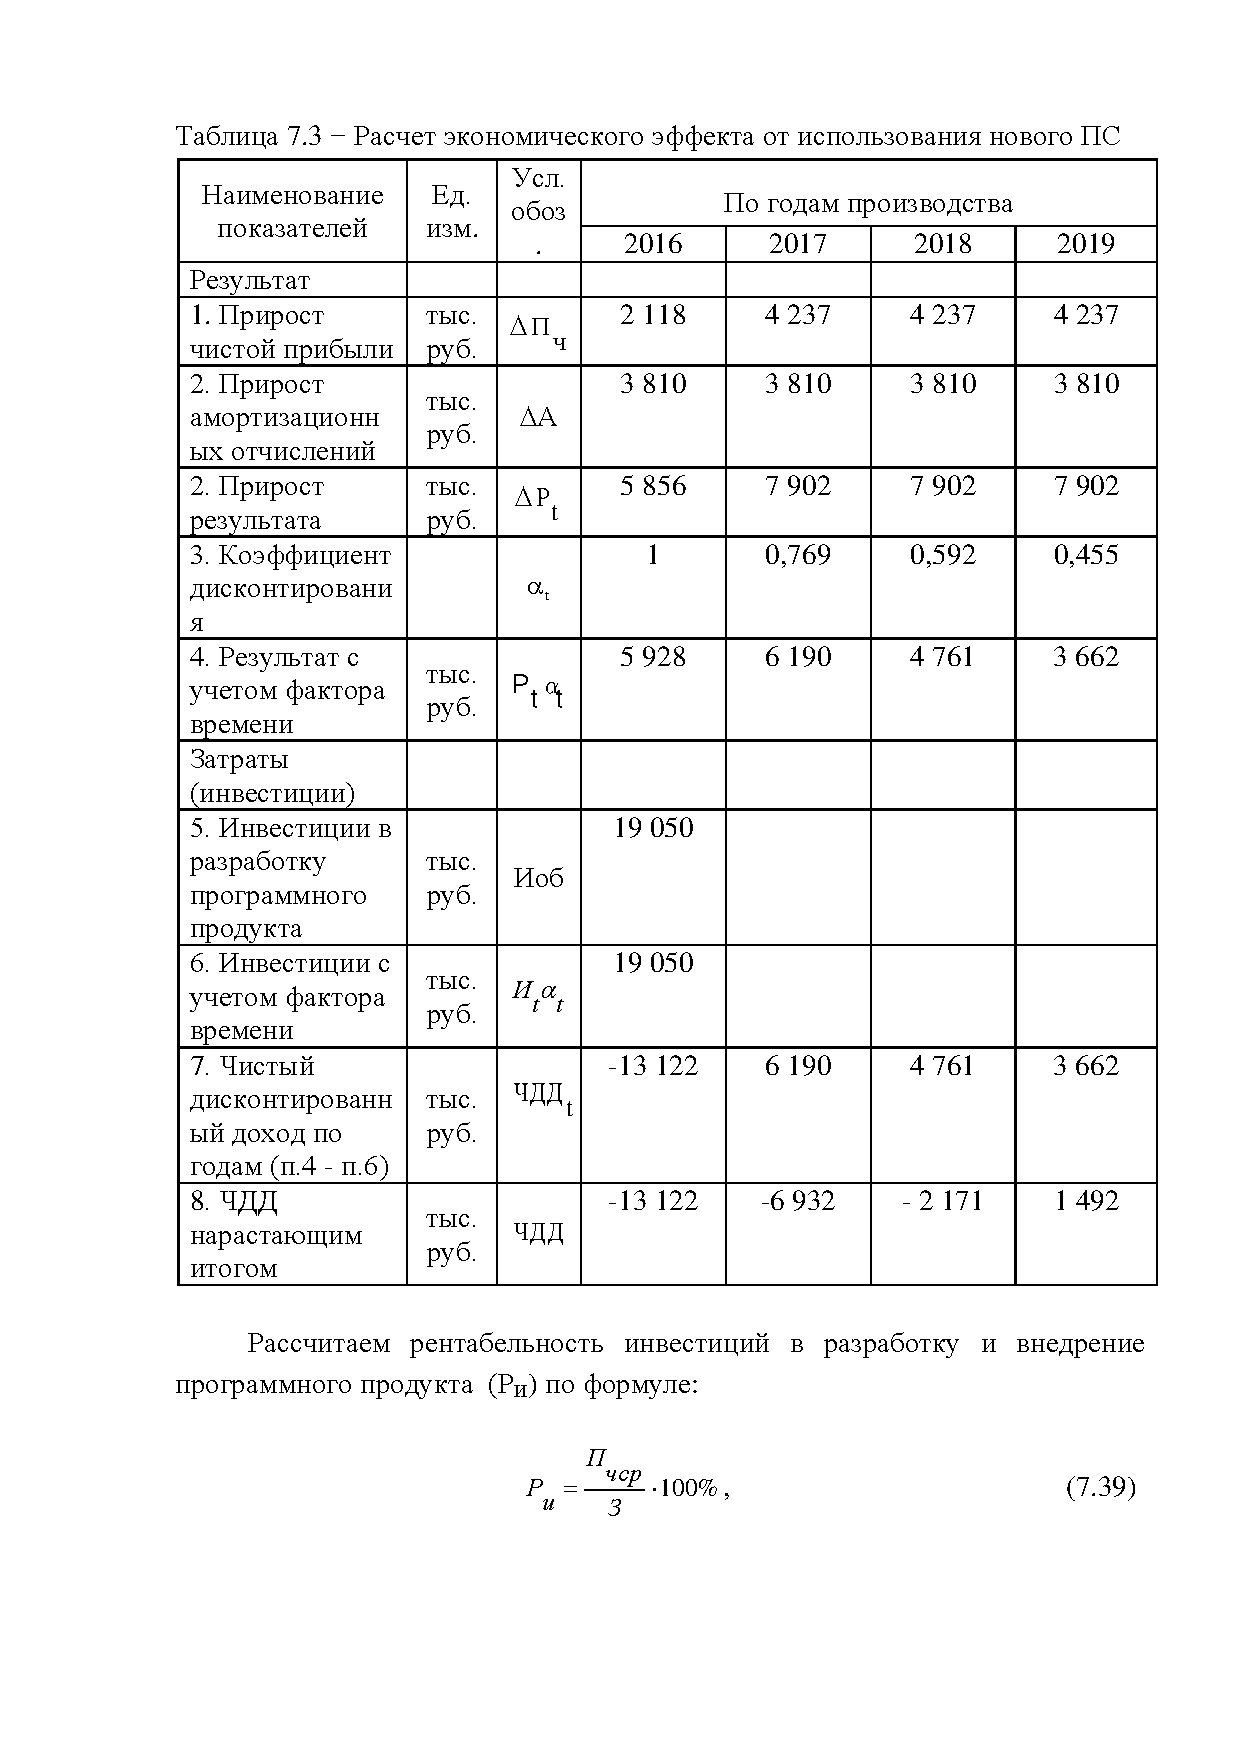
\includepdf[pages={-}]{economic_table.pdf}

% Учитывая срок разработки проекта $ \text{Т}_\text{р} = \SI{\developmentTimeMonths}{\text{мес.}} = \SI{\developmentTimeYears}{\text{года}} $, общую трудоемкость и фонд эффективного времени одного работника, вычисленные ранее, можем рассчитать численность исполнителей проекта
% \begin{equation}
%   \label{eq:econ:num_of_programmers_calc}
%   \text{Ч}_\text{р} = 
%     \frac{\num{\adjustedManDays}}
%          {\num{\developmentTimeYears} \times \num{\workingDaysInYear}} 
%     \approx \SI{\requiredNumberOfProgrammers}{\text{рабочих}}.
% \end{equation}

% Вычисленные оценки показывают, что для выполнения запланированного проекта в указанные сроки необходимо два рабочих.
% Информация о работниках перечислена в таблице~\ref{table:econ:programmers}.
% \begin{table}[ht]
%   \caption{Работники, занятые в проекте}
%   \label{table:econ:programmers}
%   \begin{tabular}{| >{\centering}m{0.4\textwidth} 
%                   | >{\centering}m{0.15\textwidth} 
%                   | >{\centering}m{0.18\textwidth} 
%                   | >{\centering\arraybackslash}m{0.15\textwidth}|}
%    \hline
%    Исполнители & Разряд & Тарифный коэффициент & \mbox{Чел./дн.} занятости \\
%    \hline
%    Программист \Rmnum{1}-категории & $ \num{13} $ & $ \num{\tariffFactorFst} $ & $ \num{\employmentFst} $ \\
%    \hline
%    Ведущий программист & $ \num{15} $ & $ \num{\tariffFactorSnd} $ & $ \num{\employmentSnd} $ \\
%    \hline
%   \end{tabular}
% \end{table}

% Месячная тарифная ставка одного работника вычисляется по формуле
% \begin{equation}
%   \label{eq:econ:month_salary}
%   \text{Т}_\text{ч} = 
%     \frac {\text{Т}_{\text{м}_{1}} \cdot \text{Т}_{\text{к}} } 
%           {\text{Ф}_{\text{р}} }  \text{\,,}
% \end{equation}
% \begin{explanation}
% где & $ \text{Т}_{\text{м}_{1}} $ & месячная тарифная ставка 1-го разряда, \byr; \\
%     & $ \text{Т}_{\text{к}} $ & тарифный коэффициент, соответствующий установленному тарифному разряду; \\
%     & $ \text{Ф}_{\text{р}} $ & среднемесячная норма рабочего времени, час.
% \end{explanation}




% Подставив данные из таблицы~\ref{table:econ:programmers} в формулу~(\ref{eq:econ:month_salary}), приняв значение тарифной ставки 1-го разряда $ \text{Т}_{\text{м}_{1}} = \SI{\tariffRateFirst}{\text{\byr}} $ и среднемесячную норму рабочего времени $ \text{Ф}_{\text{р}} = \SI{\workingHoursInMonth}{\text{часов}} $ получаем
% \begin{equation}
%   \label{eq:econ:month_salary_calc1}
%   \text{Т}_{\text{ч}}^{\text{прогр. \Rmnum{1}-разр.}} = \frac{ \num{\tariffRateFirst} \times \num{\tariffFactorFst} } { \num{\workingHoursInMonth} } = \SI{\salaryPerHourFst}{\text{\byr}/\text{час;}}
% \end{equation}
% \begin{equation}
%   \label{eq:econ:month_salary_calc2}
%   \text{Т}_{\text{ч}}^{\text{вед. прогр.}} = \frac{ \num{\tariffRateFirst} \times \num{\tariffFactorSnd} } { \num{\workingHoursInMonth} } = \SI{\salaryPerHourSnd}{\text{\byr}/\text{час.}}
% \end{equation}

% Основная заработная плата исполнителей на конкретное ПО рассчитывается по формуле 
% \begin{equation}
%   \label{eq:econ:total_salary}
%   \text{З}_{\text{о}} = \sum^{n}_{i = 1} 
%                         \text{Т}_{\text{ч}}^{i} \cdot
%                         \text{Т}_{\text{ч}} \cdot
%                         \text{Ф}_{\text{п}} \cdot
%                         \text{К}
%                           \text{\,,}
% \end{equation}
% \begin{explanation}
% где & $ \text{Т}_{\text{ч}}^{i} $ & часовая тарифная ставка \mbox{$ i $-го} исполнителя, \byr$/$час; \\
%     & $ \text{Т}_{\text{ч}} $ & количество часов работы в день, час; \\
%     & $ \text{Ф}_{\text{п}} $ & плановый фонд рабочего времени \mbox{$ i $-го} исполнителя, дн.; \\
%     & $ \text{К} $ & коэффициент премирования.
% \end{explanation}

% Подставив ранее вычисленные значения и данные из таблицы~\ref{table:econ:programmers} в формулу~(\ref{eq:econ:total_salary}) и приняв коэффициент премирования $ \text{К} = \num{\bonusRate} $ получим
% \begin{equation}
%   \label{eq:econ:total_salary_calc}
%   \text{З}_{\text{о}} = (\salaryPerHourFst \times \num{\employmentFst} + \salaryPerHourSnd \times \num{\employmentSnd}) \times \num{\workingHoursInDay} \times \num{\bonusRate} = \SI{\totalSalary}{\text{\byr}} \text{\,.}
% \end{equation}

% Дополнительная заработная плата включает выплаты предусмотренные законодательством от труде и определяется по нормативу в процентах от основной заработной платы
% \begin{equation}
%   \label{eq:econ:additional_salary}
%   \text{З}_{\text{д}} = 
%     \frac {\text{З}_{\text{о}} \cdot \text{Н}_{\text{д}}} 
%           {100\%} \text{\,,}
% \end{equation}
% \begin{explanation}
%   где & $ \text{Н}_{\text{д}} $ & норматив дополнительной заработной платы, $ \% $.
% \end{explanation}

% Приняв норматив дополнительной заработной платы $ \text{Н}_{\text{д}} = \num{\additionalSalaryNormative\%} $ и подставив известные данные в формулу~(\ref{eq:econ:additional_salary}) получим
% \begin{equation}
%   \label{eq:econ:additional_salary_calc}
%   \text{З}_{\text{д}} = 
%     \frac{\num{\totalSalary} \times 20\%}
%          {100\%} \approx \SI{\additionalSalary}{\text{\byr}} \text{\,.}
% \end{equation}

% Согласно действующему законодательству отчисления в фонд социальной защиты населения составляют \num{\socialProtectionNormative\%} , в фонд обязательного страхования "--- \num{\socialNeedsNormative\%}, от фонда основной и дополнительной заработной платы исполнителей.
% Общие отчисления на социальную защиту рассчитываются по формуле
% \begin{equation}
%   \label{eq:econ:soc_prot}
%   \text{З}_{\text{сз}} = 
%     \frac{(\text{З}_{\text{о}} + \text{З}_{\text{д}}) \cdot \text{Н}_{\text{сз}}}
%          {\num{100\%}} \text{\,.}
% \end{equation}

% Подставив вычисленные ранее значения в формулу~(\ref{eq:econ:soc_prot}) получаем
% \begin{equation}
%   \label{eq:econ:soc_prot_calc}
%   \text{З}_{\text{сз}} =
%     \frac{ (\num{\totalSalary} + \num{\additionalSalary}) \times \num{\socialProtectionFund\%} }
%          { \num{100\%} }
%     \approx \SI{\socialProtectionCost}{\text{\byr}} \text{\,.}
% \end{equation}

% \begin{comment}
%   Расчет налогов от фонда оплаты труда производится формуле
%   \begin{equation}
%     \label{eq:econ:tax_work_prot}
%     \text{Н}_{\text{е}} = 
%       \frac{(\text{З}_{\text{о}} + \text{З}_{\text{д}}) \cdot \text{Н}_{\text{не}}}
%            {\num{100\%}} \text{\,,}
%   \end{equation}
%   \begin{explanation}
%     где & $ \text{Н}_{\text{не}} $ & норматив налога, уплачиваемый единым платежом, $ \% $.
%   \end{explanation}

%   Подставив ранее вычисленные значения в формулу~(\ref{eq:econ:tax_work_prot}) и приняв норматив налога $ \text{Н}_{\text{не}} = \num{\taxWorkProtNormative\%} $ получаем
%   \begin{equation}
%     \label{eq:econ:tax_work_prot_calc}
%     \text{Н}_{\text{е}} = 
%         \frac{ (\num{\totalSalary} + \num{\additionalSalary}) \times \num{\taxWorkProtNormative\%} }
%            { \num{100\%} }
%       \approx \SI{\taxWorkProtCost}{\text{\byr}}\text{\,.}
%   \end{equation}
% \end{comment}

% По статье <<материалы>> проходят расходы на носители информации, бумагу, краску для принтеров и другие материалы, используемые при разработке ПО.
% Норма расходов $ \text{Н}_{\text{мз}} $ определяется либо в расчете на \num{100} строк исходного кода, либо в процентах к основной зарплате исполнителей \mbox{\num{3\%}\,---\,\num{5\%}}.
% Затраты на материалы вычисляются по формуле
% \begin{equation}
%   \label{eq:econ:stuff}
%   \text{М} = 
%     \frac{ \text{З}_{\text{о}} \cdot \text{Н}_{\text{мз}} }
%          { \num{100\%} } =
%     \frac{ \num{\totalSalary} \times \num{\stuffNormative\%} }
%          { \num{100\%} } \approx
%     \SI{\stuffCost}{\text{\byr}} \text{\,.}
% \end{equation}

% Расходы по статье <<машинное время>> включают оплату машинного времени, необходимого для разработки и отладки ПО, которое определяется по нормативам в машино-часах на \num{100} строк исходного кода в зависимости от характера решаемых задач и типа ПК, и вычисляются по формуле
% \begin{equation}
%   \label{eq:econ:machine_time}
%   \text{Р}_{\text{м}} =
%     \text{Ц}_{\text{м}} \cdot 
%     \frac {\text{V}_{\text{о}}}
%           {\num{100}} \cdot
%     \text{Н}_{\text{мв}} \text{\,,}
% \end{equation}
% \begin{explanation}
%   где & $ \text{Ц}_{\text{м}} $ & цена одного часа машинного времени, \byr; \\
%       & $ \text{Н}_{\text{мв}} $ & норматив расхода машинного времени на отладку 100 строк исходного кода, часов.
% \end{explanation}

% Согласно нормативу~\cite[с.\,69, приложениe~6]{palicyn_2006} норматив расхода машинного времени на отладку \num{100} строк исходного кода составляет $ \text{Н}_{\text{мв}} = \num{\timeToDebugCodeNormative} $, применяя понижающий коэффициент \num{\reducingTimeToDebugFactor} получаем $ {\text{Н}'}_{\text{мв}} = \num{\adjustedTimeToDebugCodeNormative} $.
% Цена одного часа машинного времени составляет $ \text{Ц}_{\text{м}} = \SI{\oneHourMachineTimeCost}{\text{\byr}} $.
% Подставляя известные данные в формулу~(\ref{eq:econ:machine_time}) получаем
% \begin{equation}
%   \label{eq:econ:machine_time_calc}
%   \text{Р}_{\text{м}} =
%     \num{\oneHourMachineTimeCost} \times 
%     \frac {\num{\totalProgramSizeCorrected}}
%           {\num{100}} \times
%     \num{\adjustedTimeToDebugCodeNormative} =
%     \SI{\machineTimeCost}{\text{\byr}} \text{\,.}
% \end{equation}

% Расходы по статье <<научные командировки>> вычисляются как процент от основной заработной платы, либо определяются по нормативу. 
% Вычисления производятся по формуле
% \begin{equation}
%   \label{eq:econ:business_trip}
%   \text{Р}_{\text{к}} =
%     \frac{ \text{З}_{\text{о}} \cdot \text{Н}_{\text{к}} }
%          { \num{100\%} } \text{\,,}
% \end{equation}
% \begin{explanation}
%   где & $ \text{Н}_{\text{к}} $ & норматив командировочных расходов по отношению к основной заработной плате, $ \% $.
% \end{explanation}

% Подставляя ранее вычисленные значения в формулу~(\ref{eq:econ:business_trip}) и приняв значение $ \text{Н}_{\text{к}} = \num{\businessTripNormative\%} $ получаем
% \begin{equation}
%   \label{eq:econ:business_trip_calc}
%     \text{Р}_{\text{к}} =
%     \frac{ \num{\totalSalary} \times \num{\businessTripNormative\%} }
%          { \num{100\%} } = \SI{\businessTripCost}{\text{\byr}} \text{\,.}
% \end{equation}

% Статья расходов <<прочие затраты>> включает в себя расходы на приобретение и подготовку специальной научно-технической информации и специальной литературы.
% Затраты определяются по нормативу принятому в организации в процентах от основной заработной платы и вычисляются по формуле
% \begin{equation}
%   \label{eq:econ:other_cost}
%   \text{П}_{\text{з}} =
%     \frac{ \text{З}_{\text{о}} \cdot \text{Н}_{\text{пз}} }
%          { \num{100\%} } \text{\,,}
% \end{equation}
% \begin{explanation}
%   где & $ \text{Н}_{\text{пз}} $ & норматив прочих затрат в целом по организации, $ \% $.
% \end{explanation}

% Приняв значение норматива прочих затрат $ \text{Н}_{\text{пз}} = \num{\otherCostNormative\%} $ и подставив вычисленные ранее значения в формулу~(\ref{eq:econ:other_cost}) получаем
% \begin{equation}
%   \label{eq:econ:other_cost_calc}
%   \text{П}_{\text{з}} =
%     \frac{ \num{\totalSalary} \times \num{\otherCostNormative\%} }
%          { \num{100\%} } = 
%     \SI{\otherCost}{\text{\byr}} \text{\,.}
% \end{equation}

% Статья <<накладные расходы>> учитывает расходы, необходимые для содержания аппарата управления, вспомогательных хозяйств и опытных производств, а также расходы на общехозяйственные нужны. Данная статья затрат рассчитывается по нормативу от основной заработной платы и вычисляется по формуле.

% \begin{equation}
%   \label{eq:econ:overhead_cost}
%   \text{Р}_{\text{н}} =
%     \frac{ \text{З}_{\text{о}} \cdot \text{Н}_{\text{рн}} }
%          { \num{100\%} } \text{\,,}
% \end{equation}
% \begin{explanation}
%   где & $ \text{Н}_{\text{рн}} $ & норматив накладных расходов в организации,~$ \% $.
% \end{explanation}

% Приняв норму накладных расходов $ \text{Н}_{\text{рн}} = \num{\overheadCostNormative\%} $ и подставив известные данные в формулу~(\ref{eq:econ:overhead_cost}) получаем
% \begin{equation}
%   \label{eq:econ:overhead_cost_calc}
%   \text{Р}_{\text{н}} =
%     \frac{ \num{\totalSalary} \times \num{\overheadCostNormative\%} }
%          { \num{100\%} } = 
%     \SI{\overheadCost}{\text{\byr}} \text{\,.}
% \end{equation}

% Общая сумма расходов по смете на ПО рассчитывается по формуле
% \begin{equation}
%   \label{eq:econ:overall_cost}
%   \text{С}_{\text{р}} =
%     \text{З}_{\text{о}} +
%     \text{З}_{\text{д}} +
%     \text{З}_{\text{сз}} +
%     %\text{Н}_{\text{е}} +
%     \text{М} +
%     % \text{Р}_{\text{с}} + % спецоборудование не нужно
%     \text{Р}_{\text{м}} +
%     \text{Р}_{\text{нк}} +
%     \text{П}_{\text{з}} +
%     \text{Р}_{\text{н}}\text{\,.}
% \end{equation}

% Подставляя ранее вычисленные значения в формулу~(\ref{eq:econ:overall_cost}) получаем

% \begin{equation}
%   \label{eq:econ:overall_cost_calc}
%   \text{С}_{\text{р}} = \SI{\overallCost}{\text{\byr}} \text{\,.}
% \end{equation}

% Расходы на сопровождение и адаптацию, которые несет производитель ПО, вычисляются по нормативу от суммы расходов по смете и рассчитываются по формуле
% \begin{equation}
%   \label{eq:econ:software_support}
%   \text{Р}_{\text{са}} = 
%     \frac { \text{С}_{\text{р}} \cdot \text{Н}_{\text{рса}} }
%           { \num{100\%} } \text{\,,}
% \end{equation}
% \begin{explanation}
%   где & $ \text{Н}_{\text{рса}} $ & норматив расходов на сопровождение и адаптацию ПО,~$ \% $.
% \end{explanation}

% Приняв значение норматива расходов на сопровождение и адаптацию $ \text{Н}_{\text{рса}} = \num{\supportNormative\%} $ и подставив ранее вычисленные значения в формулу~(\ref{eq:econ:software_support}) получаем
% \begin{equation}
%   \label{eq:econ:software_support_calc}
%   \text{Р}_{\text{са}} = 
%     \frac { \num{\overallCost} \times \num{\supportNormative\%} }
%           { \num{100\%} } \approx \SI{\softwareSupportCost}{\text{\byr}} \text{\,.}
% \end{equation}

% Полная себестоимость создания ПО включает сумму затрат на разработку, сопровождение и адаптацию и вычисляется по формуле
% \begin{equation}
%   \label{eq:econ:base_cost}
%   \text{С}_{\text{п}} = \text{С}_{\text{р}} + \text{Р}_{\text{са}} \text{\,.}
% \end{equation}

% Подставляя известные значения в формулу~(\ref{eq:econ:base_cost}) получаем
% \begin{equation}
%   \label{eq:econ:base_cost_calc}
%   \text{С}_{\text{п}} = \num{\overallCost} + \num{\softwareSupportCost} = \SI{\baseCost}{\text{\byr}} \text{\,.}
% \end{equation}



% \subsection{Расчёт экономической эффективности у разработчика}

% Важная задача при выборе проекта для финансирования это расчет экономической эффективности проектов и выбор наиболее выгодного проекта.
% \begin{comment}
%   Оценка коммерческой эффективности проектов ПО предполагает:
%   \begin{itemize}
%     \item определение расчётного периода и расчётных шагов проекта; 
%     \item обоснование цены ПО;
%     \item определение денежных потоков с включением всех денежных поступлений по проекту в ходе его осуществления; 
%     \item учёт изменения стоимости денег во времени;
%     \item оценку затрат и результатов по проекту в соответствии с  принципом <<без проекта>> и <<с проектом>>; 
%     \item оценку инфляции и риска;
%     \item учёт налогов, сборов, отчислений и льгот, предусмотренных законодательными нормами, действующими в расчётном периоде.
%   \end{itemize}
% \end{comment}
% Разрабатываемое ПО является заказным, т.\,е.~разрабатывается для одного заказчика на заказ.
% На основании анализа рыночных условий и договоренности с заказчиком об отпускной цене прогнозируемая рентабельность проекта составит~$ \text{У}_{\text{рп}} = \num{\profitability\%} $.
% Прибыль рассчитывается по формуле
% \begin{equation}
%   \label{eq:econ:income}
%   \text{П}_{\text{с}} = 
%     \frac { \text{С}_{\text{п}} \cdot \text{У}_{\text{рп}} }
%           { \num{100\%} } \text{\,,}
% \end{equation}
% \begin{explanation}
%   где & $ \text{П}_{\text{с}} $ & прибыль от реализации ПО заказчику, \byr; \\
%       & $ \text{У}_{\text{рп}} $ & уровень рентабельности ПО,~$ \% $.
% \end{explanation}

% Подставив известные данные в формулу~(\ref{eq:econ:income}) получаем прогнозируемую прибыль от реализации ПО
% \begin{equation}
%   \label{eq:econ:income_calc}
%   \text{П}_{\text{с}} = 
%     \frac { \num{\baseCost} \times \num{\profitability\%} }
%           { \num{100\%} } 
%     \approx \SI{\income}{\text{\byr}} \text{\,.}
% \end{equation}

% Прогнозируемая цена ПО без учета налогов включаемых в цену вычисляется по формуле 
% \begin{equation}
%   \label{eq:econ:estimated_price}
%   \text{Ц}_{\text{п}} = \text{С}_{\text{п}} + \text{П}_{\text{с}}  \text{\,.}
% \end{equation}

% Подставив данные в формулу~(\ref{eq:econ:estimated_price}) получаем цену ПО без налогов
% \begin{equation}
%   \label{eq:econ:estimated_price_calc}
%   \text{Ц}_{\text{п}} = \num{\baseCost}  + \num{\income} = \SI{\estimatedPrice}{\text{\byr}} \text{\,.}
% \end{equation}

% \begin{comment}
%   Отчисления и налоги в местный и республиканский бюджеты вычисляются по формуле
%   \begin{equation}
%     \label{eq:econ:local_repub_tax}
%     \text{О}_{\text{мр}} =
%       \frac { \text{Ц}_{\text{п}} \cdot \text{Н}_{\text{мр}} }
%             { \num{100\%} - \text{Н}_{\text{мр}} } \text{\,,}
%   \end{equation}
%   \begin{explanation}
%     где & $ \text{Н}_{\text{мр}} $ & норматив отчислений в местный и республиканский бюджеты, \byr.
%   \end{explanation}

%   Приняв норматив отчислений в местный и республиканский бюджеты $ \text{Н}_{\text{мр}} = \num{\localRepubTaxNormative\%} $ и подставив известные данные в формулу~(\ref{eq:econ:local_repub_tax}) получим величину единого платежа
%   \begin{equation}
%     \label{eq:econ:local_repub_tax_calc}
%     \text{О}_{\text{мр}} = 
%       \frac { \num{\estimatedPrice} \cdot \num{\localRepubTaxNormative\%} }
%             { \num{100\%} - \num{\localRepubTaxNormative\%} } 
%       \approx \SI{\localRepubTax}{\text{\byr}} \text{\,.}
%   \end{equation}
% \end{comment}

% Налог на добавленную стоимость рассчитывается по формуле
% \begin{equation}
%   \label{eq:econ:nds}
%   \text{НДС}_{\text{}} =
%     \frac{ \text{Ц}_{\text{п}} \cdot \text{Н}_{\text{дс}} }
%          { \num{100\%} } \text{\,,}
% \end{equation}
% \begin{explanation}
%   где & $ \text{Н}_{\text{дс}} $ & норматив НДС,~$\%$.
% \end{explanation}

% Норматив НДС составляет $ \text{Н}_{\text{дс}} = \num{\ndsNormative\%} $, подставляя известные значения в формулу~(\ref{eq:econ:nds}) получаем
% \begin{equation}
%   \text{НДС} =
%     \frac { \num{\estimatedPrice} \times \num{\ndsNormative\%} }
%           { \num{100\% }} 
%     \approx \SI{\nds}{\text{\byr}} \text{\,.}
% \end{equation}

% Расчет прогнозируемой отпускной цены осуществляется по формуле 
% \begin{equation}
%   \label{eq:econ:selling_price}
%   \text{Ц}_{\text{о}} = \text{Ц}_{\text{п}} + \text{НДС} \text{\,.}
% \end{equation}

% Подставляя известные данные в формулу~(\ref{eq:econ:selling_price}) получаем прогнозируемую отпускную цену
% \begin{equation}
%   \label{eq:econ:selling_price_calc}
%   \text{Ц}_{\text{о}} = \num{\estimatedPrice} + \num{\nds} \approx \SI{\sellingPrice}{\text{\byr}} \text{\,.}
% \end{equation}


% Чистую прибыль от реализации проекта можно рассчитать по формуле
% \begin{equation}
%   \label{eq:econ:income_with_taxes}
%   \text{П}_\text{ч} = 
%     \text{П}_\text{c} \cdot
%     \left(1 - \frac{ \text{Н}_\text{п} }{ \num{100\%} } \right) \text{\,,}
% \end{equation}
% \begin{explanation}
%   где & $ \text{Н}_{\text{п}} $ & величина налога на прибыль,~$\%$.
% \end{explanation}

% Приняв значение налога на прибыль $ \text{Н}_{\text{н}} = \num{\taxForIncome\%} $ и подставив известные данные в формулу~(\ref{eq:econ:income_with_taxes}) получаем чистую прибыль
% \begin{equation}
%   \label{eq:econ:income_with_taxes_calc}
%   \text{П}_\text{ч} = 
%     \num{\income} \times \left( 1 - \frac{\num{\taxForIncome\%}}{100\%} \right) = \SI{\incomeWithTaxes}{\text{\byr}} \text{\,.}
% \end{equation}

% Программное обеспечение разрабатывалось для одного заказчика в связи с этим экономическим эффектом разработчика будет являться чистая прибыль от реализации~$ \text{П}_\text{ч} $.
% Рассчитанные данные приведены в таблице~\ref{table:econ:calculated_data}.
% Таким образом было произведено технико"=экономическое обоснование разрабатываемого проекта, составлена смета затрат и рассчитана прогнозируемая прибыль, и показана экономическая целесообразность разработки.

% \begin{table}[!h!t]
% \caption{Рассчитанные данные}
% \label{table:econ:calculated_data}
%   \centering
%   \begin{tabular}{| >{\raggedright}m{0.60\textwidth} 
%                   | >{\centering}m{0.17\textwidth} 
%                   | >{\centering\arraybackslash}m{0.15\textwidth}|}
%     \hline
%     {\begin{center}
%       Наименование
%     \end{center} } & Условное обозначение & Значение \\
%     \hline
%     Нормативная трудоемкость, чел.$/$дн. & $ \text{Т}_\text{н} $ & \num{\normativeManDays} \\

%     \hline
%     Общая трудоемкость разработки, чел.$/$дн. & $ \text{Т}_\text{о} $ & \num{\adjustedManDays} \\

%     \hline
%     Численность исполнителей, чел. & $ \text{Ч}_\text{р} $ & \num{\requiredNumberOfProgrammers} \\

%     \hline
%     Часовая тарифная ставка программиста \Rmnum{1}-разряда, \byr{}$/$ч. & $ \text{Т}_{\text{ч}}^{\text{прогр. \Rmnum{1}-разр.}} $ & \num{\salaryPerHourFst} \\

%     \hline
%     Часовая тарифная ставка ведущего программиста, \byr{}$/$ч. & $ \text{Т}_{\text{ч}}^{\text{вед. прогр.}} $ & \num{\salaryPerHourSnd} \\

%     \hline
%     Основная заработная плата, \byr{} & $ \text{З}_\text{о} $ & \num{\totalSalary} \\

%     \hline
%     Дополнительная заработная плата, \byr{} & $ \text{З}_\text{д}$ & \num{\additionalSalary} \\

%     \hline
%     Отчисления в фонд социальной защиты, \byr{} & $ \text{З}_\text{сз} $ & \num{\socialProtectionCost} \\

%     \hline
%     Затраты на материалы, \byr{} & $ \text{М} $ & \num{\stuffCost} \\

%     \hline
%     Расходы на машинное время, \byr{} & $ \text{Р}_\text{м} $ & \num{\machineTimeCost} \\

%     \hline
%     Расходы на командировки, \byr{} & $ \text{Р}_\text{к} $ & \num{\businessTripCost} \\

%     \hline
%     Прочие затраты, \byr{} & $ \text{П}_\text{з} $ & \num{\otherCost} \\

%     \hline
%     Накладные расходы, \byr{} & $ \text{Р}_\text{н} $ & \num{\overheadCost} \\

%     \hline
%     Общая сумма расходов по смете, \byr{} & $ \text{С}_\text{р} $ & \num{\overallCost} \\

%     \hline
%     Расходы на сопровождение и адаптацию, \byr{} & $ \text{Р}_\text{са} $ & \num{\softwareSupportCost} \\

%     \hline
%     Полная себестоимость, \byr{} & $ \text{С}_\text{п} $ & \num{\baseCost} \\

%     \hline
%     Прогнозируемая прибыль, \byr{} & $ \text{П}_\text{с} $ & \num{\income} \\

%     \hline
%     НДС, \byr{} & $ \text{НДС} $ & \num{\nds} \\

%     \hline
%     Прогнозируемая отпускная цена ПО, \byr{} & $ \text{Ц}_\text{о} $ & \num{\sellingPrice} \\

%     \hline
%     Чистая прибыль, \byr{} & $ \text{П}_\text{ч} $ & \num{\incomeWithTaxes} \\

%     \hline
%   \end{tabular}
% \end{table}
% \hfill
% \clearpage


% % Часть, которая, к сожалению, была написана, наверное, зря.
% \begin{comment}

% Договоренность с заказчиком предусматривает оплату за ПО после его адаптации на стороне заказчика. 
% Следствием из данной договоренности являются возникающие риски для организации исполнителя связанные с неуплатой стоимости проекта заказчиком.
% На случай провала сделки с определенным заказчиком рассмотрим бизнес"=план, который предусматривает массовую реализацию разрабатываемого ПО по сниженной цене, и оценим экономическую эффективность разработки с данной точки зрения.

% \FPeval{\priceFirstYear}{1500}
% \FPeval{\priceSecondYear}{1250}
% \FPeval{\priceThirdYear}{1000}
% Расчетный период для разрабатываемого проекта состоит из трех интервалов времени длительностью один год. 
% На рынке существует достаточное количество как платных так и бесплатных аналогов разрабатываемого продукта. Анализ платных продуктов показал, что начальную цену на одну лицензию целесообразно установить ниже средней на рынке в размере $ P_1 = \SI{\priceFirstYear}{\text{тыс.\,\byr}} $, в последующие отрезки времени расчетного периода $ t_2 $ и $ t_3 $ планируется планомерно снижать цену до $ P_2 = \SI{\priceSecondYear}{\text{тыс.\,\byr}} $ и $ P_3 = \SI{\priceThirdYear}{\text{тыс.\,\byr}} $ для привлечения новых клиентов.

% \FPeval{\soldInFirstYear}{30}
% \FPeval{\soldInSecondYear}{50}
% \FPeval{\soldInThirdYear}{40}
% В связи с тем, что разрабатываемое ПО не предназначено для широкого круга пользователей, то прогнозируемый уровень продаж для расчетного периода составит $ Q_1 = \num{\soldInFirstYear} $, $ Q_2 = \num{\soldInSecondYear} $ и $ Q_3 = \num{\soldInThirdYear} $ копий.

% \FPeval{\revenueInFirstYear}{clip(\soldInFirstYear * \priceFirstYear)}
% \FPeval{\revenueInSecondYear}{clip(\soldInSecondYear * \priceSecondYear)}
% \FPeval{\revenueInThirdYear}{clip(\soldInThirdYear * \priceThirdYear)}
% Выручка от продаж в $i$-й отрезок времени расчетного периода вычисляется по формуле
% \begin{equation}
%   \label{eq:econ:profit}
%   \text{Д}^\text{р}_i = P_i \cdot Q_i \text{\,.}
% \end{equation}

% Рассчитанные данные приведены в таблице~\ref{table:econ:justification}. Входной денежный поток в $i$-й отрезок времени расчетного периода рассчитывается по формуле
% \begin{equation}
%   \label{eq:econ:income_cash_flow}
%   \text{ДП}^\text{п}_i = \text{Д}^\text{р}_i + \text{А}^\text{о}_i \text{\,.}
% \end{equation}
% \begin{explanation}
% где & $ \text{А}^\text{о}_i $ & амортизационные отчисления, \byr.
% \end{explanation}

% \FPeval{\depreciations}{3000}
% \FPeval{\firstYearCashFlowIncome}{clip(\depreciations + \revenueInFirstYear)}
% \FPeval{\secondYearCashFlowIncome}{clip(\depreciations + \revenueInSecondYear)}
% \FPeval{\thirdYearCashFlowIncome}{clip(\depreciations + \revenueInThirdYear)}

% Выходной денежный поток рассчитывается в $i$-й отрезок времени расчетного периода вычисляется по формуле
% \begin{equation}
%   \label{eq:econ:cash_flow_outcome}
%   \text{ДП}^\text{о}_i = \text{Р}^\text{п}_i + \text{Р}^\text{у}_i + \text{Р}^\text{н}_i
% \end{equation}
% \begin{explanation}
% где & $ \text{Р}^\text{п}_i $ & переменные затраты на производство и реализацию, \byr; \\
%     & $ \text{Р}^\text{у}_i $ & расходы постоянные на управление и обслуживание, \byr; \\
%     & $ \text{Р}^\text{н}_i $ & налоги, уплачиваемые из прибыли.
% \end{explanation}

% Прогнозируемые постоянные и переменные затраты, а также налоги и выходные денежные потоки приведены в таблице~\ref{table:econ:justification}. Норматив налога на прибыль принят $ \text{Н}_\text{нп} = \num{12\%} $. 

\FPeval{\firstYearVariableCosts}{17200}
\FPeval{\secondYearVariableCosts}{18300}
\FPeval{\thirdYearVariableCosts}{15800}

\FPeval{\firstYearConstCosts}{12000}
\FPeval{\secondYearConstCosts}{11100}
\FPeval{\thirdYearConstCosts}{9400}

\FPeval{\firstYearCostOfProduction}{clip(\firstYearVariableCosts + \firstYearConstCosts)}
\FPeval{\secondYearCostOfProduction}{clip(\secondYearVariableCosts + \secondYearConstCosts)}
\FPeval{\thirdYearCostOfProduction}{clip(\thirdYearVariableCosts + \thirdYearConstCosts)}

\FPeval{\firstYearGrossProfit}{clip(\revenueInFirstYear - \firstYearCostOfProduction)}
\FPeval{\secondYearGrossProfit}{clip(\revenueInSecondYear - \secondYearCostOfProduction)}
\FPeval{\thirdYearGrossProfit}{clip(\revenueInThirdYear - \thirdYearCostOfProduction)}

\FPeval{\firstYearPropertyTax}{300}
\FPeval{\secondYearPropertyTax}{300}
\FPeval{\thirdYearPropertyTax}{300}

\FPeval{\firstYearTaxableIncome}{clip(\firstYearGrossProfit - \firstYearPropertyTax)}
\FPeval{\secondYearTaxableIncome}{clip(\secondYearGrossProfit - \secondYearPropertyTax)}
\FPeval{\thirdYearTaxableIncome}{clip(\thirdYearGrossProfit - \thirdYearPropertyTax)}

\FPeval{\incomeTax}{0.12}
\FPeval{\fyIncomeTax}{clip(\firstYearTaxableIncome * \incomeTax)}
\FPeval{\syIncomeTax}{clip(\secondYearTaxableIncome * \incomeTax)}
\FPeval{\tyIncomeTax}{clip(\thirdYearTaxableIncome * \incomeTax)}

\FPeval{\fyNetIncome}{clip(\firstYearTaxableIncome - \fyIncomeTax)}
\FPeval{\syNetIncome}{clip(\secondYearTaxableIncome - \syIncomeTax)}
\FPeval{\tyNetIncome}{clip(\thirdYearTaxableIncome - \tyIncomeTax)}

\FPeval{\capitalInvestments}{clip(\baseCost / 1000)}
\FPround\capitalInvestments{\capitalInvestments}{0}

\FPeval{\discountRate}{0.295}

\FPeval{\zyDiscountFactor}{1}
\FPeval{\fyDiscountFactor}{clip(\zyDiscountFactor / (1 + \discountRate))}
\FPeval{\syDiscountFactor}{clip(\fyDiscountFactor / (1 + \discountRate))}
\FPeval{\tyDiscountFactor}{clip(\syDiscountFactor / (1 + \discountRate))}


\FPeval{\fyCashFlowOutcome}{clip(\firstYearCostOfProduction + \firstYearPropertyTax + \fyIncomeTax)}
\FPeval{\syCashFlowOutcome}{clip(\secondYearCostOfProduction + \secondYearPropertyTax + \syIncomeTax)}
\FPeval{\tyCashFlowOutcome}{clip(\thirdYearCostOfProduction + \thirdYearPropertyTax + \tyIncomeTax)}

\FPeval{\fyCashFlowOutcomeDiscounted}{clip(\fyCashFlowOutcome * \fyDiscountFactor)}
\FPeval{\syCashFlowOutcomeDiscounted}{clip(\syCashFlowOutcome * \syDiscountFactor)}
\FPeval{\tyCashFlowOutcomeDiscounted}{clip(\tyCashFlowOutcome * \tyDiscountFactor)}

\FPeval{\fyCashFlowIncomeDiscounted}{clip(\firstYearCashFlowIncome * \fyDiscountFactor)}
\FPeval{\syCashFlowIncomeDiscounted}{clip(\secondYearCashFlowIncome * \syDiscountFactor)}
\FPeval{\tyCashFlowIncomeDiscounted}{clip(\thirdYearCashFlowIncome * \tyDiscountFactor)}

\FPround\fyDiscountFactor{\fyDiscountFactor}{3}
\FPround\syDiscountFactor{\syDiscountFactor}{3}
\FPround\tyDiscountFactor{\tyDiscountFactor}{3}

\FPround\fyCashFlowIncomeDiscounted{\fyCashFlowIncomeDiscounted}{0}
\FPround\syCashFlowIncomeDiscounted{\syCashFlowIncomeDiscounted}{0}
\FPround\tyCashFlowIncomeDiscounted{\tyCashFlowIncomeDiscounted}{0}

\FPround\fyCashFlowOutcomeDiscounted{\fyCashFlowOutcomeDiscounted}{0}
\FPround\syCashFlowOutcomeDiscounted{\syCashFlowOutcomeDiscounted}{0}
\FPround\tyCashFlowOutcomeDiscounted{\tyCashFlowOutcomeDiscounted}{0}

\FPround\zyNetIncomeAcc{-\capitalInvestments}{0}
\FPeval{\fyNetIncomeAcc}{clip(\zyNetIncomeAcc + (\fyCashFlowIncomeDiscounted - \fyCashFlowOutcomeDiscounted))}
\FPeval{\syNetIncomeAcc}{clip(\fyNetIncomeAcc + (\syCashFlowIncomeDiscounted - \syCashFlowOutcomeDiscounted))}
\FPeval{\tyNetIncomeAcc}{clip(\syNetIncomeAcc + (\tyCashFlowIncomeDiscounted - \tyCashFlowOutcomeDiscounted))}


% Для оценки изменения стоимости денег необходимо оценить норму дисконта, которая вычисляется по формуле
% \begin{equation}
%   \label{eq:econ:discount_rate}
%   \text{Е} = r + s + \sum_{i=1}^{n} g_i \text{\,,}
% \end{equation}
% \begin{explanation}
% где & $ r $ & реальная (без учета компенсации за инфляцию) безрисковая ставка ссудного процента, \%; \\
%     & $ s $ & инфляционное ожидание за период $ t $, рассчитанное как среднее за расчетный период проекта, \%; \\
%     & $ g_i $ & премия за отдельный риск по конкретному фактору, \%.
% \end{explanation}

% Примем во внимание экономическую обстановку в Беларуси на начало 2013 года, чтобы получить значения коэффициента дисконтирования. 
% Безрисковая ставка ссудного процента составляет $r = \num{5.5\%}$, возможное влияние непредвиденных обстоятельств на величину этой ставки оценим премией за риск $ g_1 = \num{1\%} $.
% По различным данным инфляция в 2013 году в Беларуси составит $ s = \num{21\%} $. Дополнительно учтем риски падения спроса $ g_2 = \num{1\%} $ и падения дохода $ g_3 = \num{1\%}$.
% Подставляя приведенные данные в формулу~(\ref{eq:econ:discount_rate}) получаем
% \begin{equation}
%   \label{eq:econ:discount_rate_calc}
%   \text{Е} = \num{5.5\%} + \num{21\%} + \num{1\%} + \num{1\%} + \num{1\%} = \num{29.5\%} \text{\,.}
% \end{equation}

% Зная норму дисконта можно рассчитать значения коэффициентов дисконтирования для каждого из отрезков времени расчетного периода по формуле~(\ref{eq:econ:discount_factor}). Рассчитанные коэффициенты приведены в таблице~\ref{table:econ:justification}.
% \begin{equation}
%   \label{eq:econ:discount_factor}
%   \alpha_t = (1 + \text{Е})^{-t} \text{\,,}
% \end{equation}
% \begin{explanation}
% где & $ t $ & номер отрезка времени расчетного периода с момента старта проекта, \%.
% \end{explanation}

% Основным показателем экономической целесообразности реализации проекта является чистый дисконтированный доход. 
% Разрабатываемый проект предусматривает одноразовые начальные инвестиции, поэтому чистый дисконтированный доход может быть рассчитан по формуле
% \begin{equation}
%   \label{eq:econ:net_present_value}
%   \text{ЧДД} = -\text{И}_{0} + \sum_{t = 1}^m \text{ДП}^\text{п}_i \cdot \alpha_i - \sum_{t = 1}^m \text{ДП}_\text{о}^i \cdot \alpha_i \text{\,,}
% \end{equation}

% Прогнозируемые значения ЧДД приведены в таблице~\ref{table:econ:justification}. 
% Т.\,к.~значение данного экономичекого показателя $ \text{ЧДД} > 0 $, то проект приносит прибыль.
% Мы не распологаем бухгалтерскими данными по аналогичным проектам, поэтому вычисление индекса рентабельности не несет в себе полезной нагрузки и он не может быть использован для сравнения проектов.
% С финансовой точки зрения срок окупаемости проекта является спорным показателем эффективности~\cite[с.~166\,--\,167]{crundwell_2008}, по этой и по приведенной раньше причине точный расчет данного показателя производить не будем. 
% По прогнозируемым данным приведенным в таблице~\ref{table:econ:justification} приблизительный срок окупаемости проекта составит $ \text{Т}_\text{ок} \approx \SI{2}{\text{года}} $.


% \begin{table}[ht]
% \caption{Прогнозные данные реализации проекта ПО}
% \label{table:econ:justification}
% \centering
%   \begin{tabular}{| >{\raggedright}m{0.34\textwidth} 
%                   | >{\centering}m{0.091\textwidth} 
%                   | >{\centering}m{0.105\textwidth} 
%                   | >{\centering}m{0.105\textwidth} 
%                   | >{\centering}m{0.1\textwidth} 
%                   | >{\centering\arraybackslash}m{0.1\textwidth}|}
%     \hline
%       \multirow{3}{0.34\textwidth}{\centering Показатели} &
%       \multirow{3}{0.091\textwidth}{\centering Ед. измер.} &
%       \multicolumn{4}{c|}{\centering Значения показателей по шагам} \\
    
%     \cline{3-6} 
%     & & 2013 & 2014 & 2015 & 2016 \\
%     & & $ t_0 $ & $ t_1 $ & $ t_2 $ & $ t_3 $ \\
    
%     \hline
%     1 & 2 & 3 & 4 & 5 & 6 \\
    
%     \hline
%     Объём производства и реализации & штук & & \num{\soldInFirstYear} & \num{\soldInSecondYear} & \num{\soldInThirdYear} \\ 

%     \hline
%     Прогнозная рыночная цена & тыс.\,\byr & & \num{\priceFirstYear} & \num{\priceSecondYear} & \num{\priceThirdYear} \\

%     \hline
%     Выручка от продаж (без налогов, включаемых в цену) & тыс.\,\byr & & \num{\revenueInFirstYear} & \num{\revenueInSecondYear} & \num{\revenueInThirdYear} \\

%     \hline
%     Переменные затраты & тыс.\,\byr & & \num{\firstYearVariableCosts} & \num{\secondYearVariableCosts} & \num{\thirdYearVariableCosts} \\

%     \hline
%     Постоянные затраты & тыс.\,\byr & & \num{\firstYearConstCosts} & \num{\secondYearConstCosts} & \num{\thirdYearConstCosts} \\

%     \hline
%     Затраты на производство и реализацию & тыс.\,\byr & & \num{\firstYearCostOfProduction} & \num{\secondYearCostOfProduction} & \num{\thirdYearCostOfProduction} \\

%     \hline
%     Валовая прибыль & тыс.\,\byr & & \num{\firstYearGrossProfit} & \num{\secondYearGrossProfit} & \num{\thirdYearGrossProfit} \\

%     \hline
%     Налог на недвижимость & тыс.\,\byr & & \num{\firstYearPropertyTax} & \num{\secondYearPropertyTax} & \num{\thirdYearPropertyTax} \\

%     \hline
%     Налогооблагаемая прибыль & тыс.\,\byr & & \num{\firstYearTaxableIncome} & \num{\secondYearTaxableIncome} & \num{\thirdYearTaxableIncome} \\

%     \hline
%     Налог на прибыль & тыс.\,\byr & & \num{\fyIncomeTax} & \num{\syIncomeTax} & \num{\tyIncomeTax} \\

%     \hline
%     Чистая прибыль & тыс.\,\byr & & \num{\fyNetIncome} & \num{\syNetIncome} & \num{\tyNetIncome} \\

%     \hline
%     Амортизационные отчисления & тыс.\,\byr & & \num{\depreciations} & \num{\depreciations} & \num{\depreciations} \\

%     \hline
%     Капитальные вложения & тыс.\,\byr & \num{\capitalInvestments} & & & \\

%     \hline 
%     Коэффициент дисконтирования & & \num{\zyDiscountFactor} & \num{\fyDiscountFactor} & \num{\syDiscountFactor} & \num{\tyDiscountFactor} \\

%     \hline
%     Сумма денежного притока & тыс.\,\byr & & \num{\firstYearCashFlowIncome} & \num{\secondYearCashFlowIncome} & \num{\thirdYearCashFlowIncome} \\

%     \hline
%     Сумма денежного оттока & тыс.\,\byr & \num{\capitalInvestments} & \num{\fyCashFlowOutcome} & \num{\syCashFlowOutcome} & \num{\tyCashFlowOutcome} \\

%     \hline
%     Сумма дисконтированного денежного притока & тыс.\,\byr & & \num{\fyCashFlowIncomeDiscounted} & \num{\syCashFlowIncomeDiscounted} & \num{\tyCashFlowIncomeDiscounted} \\

%     \hline 
%     Сумма дисконтированного денежного оттока & тыс.\,\byr & \num{\capitalInvestments} & \num{\fyCashFlowOutcomeDiscounted} & \num{\syCashFlowOutcomeDiscounted} & \num{\tyCashFlowOutcomeDiscounted} \\

%     \hline 
%     Сумма чистого дисконтированного денежного дохода нарастающим итогом & тыс.\,\byr & \num{\zyNetIncomeAcc} & \num{\fyNetIncomeAcc} & \num{\syNetIncomeAcc} & \num{\tyNetIncomeAcc} \\
 
%     \hline

%   \end{tabular}
% \end{table}

% \end{comment}


\sectioncentered*{Заключение}
\addcontentsline{toc}{section}{Заключение}

Итогом выполнения дипломного проекта является мобильное программное средство <<Органайзер здоровья пациента>>.

До реализации данного программного продукта были изучены подходы реализаций аналогов программного средства. Для каждого аналога были выявлены плюсы и минусы и сделаны выводы. Также был произведен анализ платформ и библиотек, для реализации клиентской части. В результате проведенного анализа и на основании требований заданных к программному средству, был определен оптимальный набор платформ и библиотек.

Для серверной части приложения был произведен анализ существующих облачных сервисов, предоставляющих возможность использовать веб-сервера и веб-сервисы. Из всех аналогов был выбран облачный сервер Amazon, который успешно подходил под все требования.

Спроектированы необходимые схемы алгоритмов и схема базы данных. Все поставленные перед разработкой цели выполнены, реализована вся функциональность, представленная в спецификации требований. Произведено тестирование разработанного программного средства с использованием модульных и интеграционных тестов.

При реализации программного продукта были использованы следующие технологии:

\begin{itemize}
  \item платформа Cordova;
  \item NodeJS для сервера приложения;
  \item ReactJS для клиентского приложения
  \item MongoDB
  \item ORM Mongoose
\end{itemize}

Также в ходе разработки дипломного проекта была рассмотрена экономическая сторона и рассчитан экономический эффект от внедрения программного средства и показатели эффективности использования программного средства у пользователя. В результате расчетов подтвердилась экономическая целесообразность разработки. 

% Зачем: Изменение надписи для списка литературы
% Почему: Пункт 2.8.1 Требований по оформлению пояснительной записки.
\renewcommand{\bibsection}{\sectioncentered*{Cписок использованных источников}}
\phantomsection\pagebreak% исправляет нумерацию в документе и исправляет гиперссылки в pdf
\addcontentsline{toc}{section}{Cписок использованных источников}

% Зачем: Печать списка литературы. База данных литературы - файл bibliography_database.bib
\bibliography{bibliography_database}


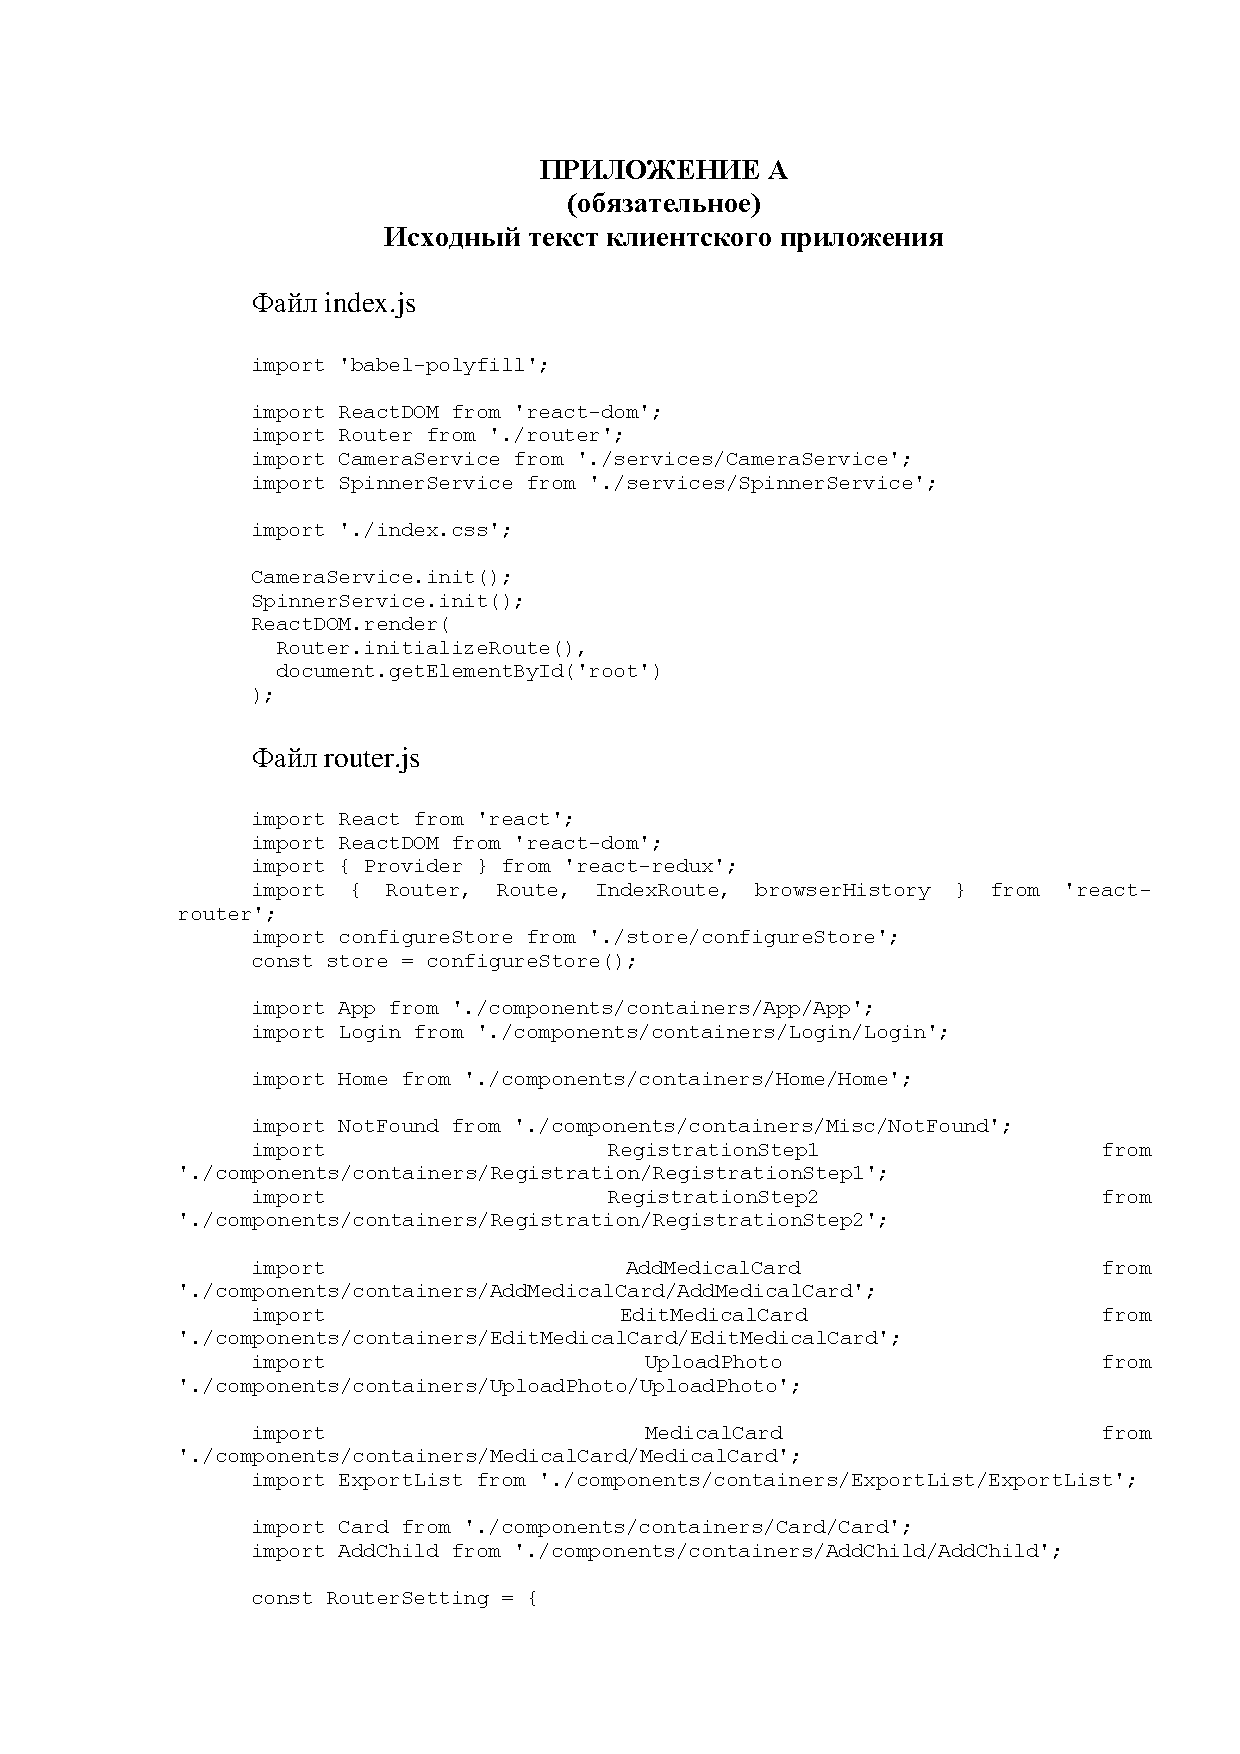
\includepdf[pages={-}, pagecommand={}]{source_code.pdf}
% \includepdf позволяет включить в результирующий pdf документ часть другого pdf документа, сделанного
% например не с помощью TeX. Бывает полезно, если какие-то диаграммны нарисованы, например, с помощью 
% Microoft Office и сохранены в pdf.
%\includepdf[pages={-}]{documents_list.pdf}

\end{document}